\documentclass[oneside,a4paper,11pt]{report}
\usepackage{fullpage}
\usepackage{hhline}

\usepackage{../../info/packages}
\usepackage{../../info/nomenclature}
\usepackage{scalerel}

\title{Flow Physics}
\author{Alejandro Campos}

\begin{document}
\maketitle
\tableofcontents

\chapter*{Preface}
\addcontentsline{toc}{chapter}{Preface}

%%%%%%%%%%%%%%%%%%%%%%%%%%%%%%%%%%%%%%%%%%%%%%%%%%%%%%%%%%%%%%%%%%%%%%%%%
\part{Governing equations}
%%%%%%%%%%%%%%%%%%%%%%%%%%%%%%%%%%%%%%%%%%%%%%%%%%%%%%%%%%%%%%%%%%%%%%%%%

%########################################################################
\chapter{Atomistic representation}
%########################################################################

%------------------------------------------------------------------------
\section{Atomistic vs.\@ fluid variables}
%------------------------------------------------------------------------
\label{sec:atomistic_and_fluid}
We'll describe fluids using variables such as $\rho=\rho(t,\xvec)$ for the fluid density, $\uvec = \uvec(t,\xvec)$ for the fluid velocity, and $e=e(t,\xvec)$ for the fluid specific internal energy, where $t$ is time and $\xvec$ is a location in space. Fluid variables are defined at every point $\xvec$ within the domain containing the fluid. Thus, in the fluid approach we do not account for the microscopic distribution of the fluid's atoms and molecules, which are not necessarily present at every point $\xvec$. That being said, we can establish a correlation between the fluid variables and atomistic variables, which define the underlying microscopic structure. Examples of these atomistic variables include $m^{(i)}$, $\uvec^{(i)}$, and $e^{(i)}$, which are the mass, velocity, and internal energy of the $i$\textsuperscript{th} atom or molecule in the system.

Consider the total mass $m_\Omega$ in some subdomain $\Omega$. This mass can be computed by summing up the masses $m^{(i)}$ of the atoms or molecules in this subdomain, or by using the Eulerian field variable for density, as shown below
\begin{equation}
   m_\Omega = \sum_{i \in \Omega} m^{(i)} = \int_{\Omega} \rho \, d\xvec.
\end{equation} 
In the above, $i \in \Omega$ denotes the atoms or molecules within the subdomain $\Omega$. Now consider the total momentum $P_\Omega$ in some subdomain $\Omega$. This momentum can be computed by summing up the momentum $m^{(i)} \uvec^{(i)}$ of the atoms or molecules in this subdomain, or by using the Eulerian field variable for velocity, as shown below
\begin{equation}
    P_\Omega = \sum_{i \in \Omega} m^{(i)} \uvec^{(i)} = \int_\Omega \rho \uvec \, d\xvec.
\end{equation}
Finally, consider the internal energy $IE_\Omega$ in some subdomain $\Omega$. This internal energy can be computed by summing up the internal energies $e^{(i)}$ of the atoms or molecules in this subdomain, or by using the Eulerian field variable for the specific internal energy, as shown below
\begin{equation}
    IE_\Omega = \sum_{i \in \Omega} e^{(i)} = \int_\Omega \rho e \, d\xvec.
\end{equation}

%------------------------------------------------------------------------
\section{Interpretation of fluid variables}
%------------------------------------------------------------------------
\label{sec:atomistic_representation}
Denote the volume of domain $\Omega$ as $V_\Omega$, which is given by
\begin{equation}
    V_\Omega = \int_\Omega d\xvec.
\end{equation}
We can now write
\begin{equation}
    \label{eq:atomistic_rho}
    \rho = \lim_{\Omega \to \epsilon} \frac{1}{V_\Omega} \int_\Omega \rho \, d\xvec = \lim_{\Omega \to \epsilon} \frac{1}{V_\Omega} \sum_{i \in \Omega} m^{(i)} = \lim_{\Omega \to \epsilon} \frac{m_\Omega}{V_\Omega}.
\end{equation}
Thus, the density is the mass contained in a small domain divided by the volume of that small domain as the domain becomes sufficiently small. Similarly for velocity, we have
\begin{equation}
    \label{eq:atomistic_u}
    \uvec = \frac{\rho\vvec}{\rho} = \lim_{\Omega \to \epsilon} \frac{\frac{1}{V_\Omega} \int_\Omega \rho \uvec \, dx}{\frac{1}{V_\Omega} \int_\Omega \rho \, dx} = \lim_{\Omega \to \epsilon} \frac{ \sum_{i \in \Omega} m^{(i)} v^{(i)} }{ \sum_{i \in \Omega} m^{(i)} } = \lim_{\Omega \to \epsilon} \frac{ P_\Omega }{ m_\Omega }.
\end{equation}
That is, the velocity is the the momentum contained in a small domain divided by the mass contained in that small domain as the domain becomes sufficiently small. Finally, for energy we have
\begin{equation}
    \label{eq:atomistic_e}
    e = \frac{\rho e}{\rho} = \lim_{\Omega \to \epsilon} \frac{ \frac{1}{V_\Omega} \int_\Omega \rho e \, d\xvec}{ \frac{1}{V_\Omega} \int_\Omega \rho \, d\xvec} = \lim_{\Omega \to \epsilon} \frac{ \sum_{i \in \Omega} e^{(i)} }{ \sum_{i \in \Omega} m^{(i)} } = \lim_{
        \Omega \to \epsilon} \frac{ IE_\Omega }{ m_\Omega }.
\end{equation}
That is, the specific internal energy is the internal energy contained in a small subdomain divided by the mass contained in that small subdomain as the subdomain becomes sufficiently small.

In the above, a sufficiently small subdomain is one that is small compared to the smallest length scale in the flow field but large enough that it contains a sufficiently large number of atoms or molecules.

%------------------------------------------------------------------------
\section{Additional atomistic variables}
%------------------------------------------------------------------------
We denote the number of atoms or molecules in some subdomain $\Omega$ as $N_\Omega$. Additionally, we denote the number of moles in some subdomain $\Omega$ as $o_\Omega$. Avogadro's number $N_a$ can thus be used to write 
\begin{equation}
    \label{eq:atomistic_particles_moles}
    N_\Omega = N_a o_\Omega.
\end{equation}
Similarly, with $M$ as the molar mass, we have
\begin{equation}
    \label{eq:atomistic_mass_moles}
    m_\Omega = M o_\Omega.
\end{equation}

Finally, we denote the number density as $n = n(t,\xvec)$, which is defined as
\begin{equation}
    \label{eq:atomistic_number_density}
    n = \lim_{\Omega \to \infty} \frac{N_\Omega}{V_\Omega}.
\end{equation}

%########################################################################
\chapter{Kinematics of fluid motion}
%########################################################################

%------------------------------------------------------------------------
\section{Eulerian and Lagrangian reference frames}
%------------------------------------------------------------------------
The Eulerian description of a fluid is that for which fluid properties are of the form $\fvec = \fvec(t,\xvec)$, where $t$ and $\xvec$ denote time and position. Examples of these include density $\rho = \rho(t,\xvec)$, fluid velocity $\uvec = \uvec(t,\xvec)$, and specific internal energy $e = e(t, \xvec)$, first mentioned in \cref{sec:atomistic_and_fluid}.

Lagrangian fields are used to describe moving particles, for which fluid properties are of the form $\fvec^+ = \fvec^+(t,\yvec)$, where $t$ denotes time and $\yvec$ the location of the particle at an initial time. Eulerian and Lagrangian properties are related to each other according to 
\begin{equation}
\fvec^+(t,\yvec)=\fvec(t,\xvec^+(t,\yvec)).
\end{equation}

There are two Lagrangian properties that deserve further attention. The position and velocity of a particle are given by $\xvec^+ = \xvec^+(t,\yvec)$ and $\vvec^+ = \vvec^+(t,\yvec)$, respectively. These two are related to each other according to 
\begin{equation}
\frac{\partial \xvec^+}{\partial t} = \vvec^+.
\end{equation}

%------------------------------------------------------------------------
\section{Material derivative}
%------------------------------------------------------------------------

We are interested in knowing how $\fvec^+(t,\yvec)$ for a hypothetical particle changes as we move along the particle's path. Applying the chain rule and product rule,
\begin{align}
\frac{\partial}{\partial t} \fvec^+(t,\yvec)&= \frac{\partial}{\partial t} \fvec(t,\xvec^+(t,\yvec)) \nonumber \\
&=  \frac{\partial}{\partial t} \fvec(t,x_1^+(t,\yvec), x_2^+(t,\yvec), x_3^+(t,\yvec)) \nonumber \\
&=\left( \frac{\partial \fvec(t,x_1,x_2,x_3)}{\partial t}\right )_{\xvec=\xvec^+(t,\yvec)} + \frac{\partial x_1^+(t,\yvec)}{\partial t} \left ( \frac{\partial \fvec(t,x_1,x_2,x_3)}{\partial x_1} \right )_{\xvec = \xvec^+(t,\yvec)} + ...\nonumber \\
&=\left ( \frac{\partial \fvec(t,x_1,x_2,x_3)}{\partial t} \right)_{\xvec=\xvec^+(t,\Yvec)} + v_1^+(t,\yvec) \left ( \frac{\partial \fvec(t,x_1,x_2,x_3)}{\partial x_1} \right )_{\xvec=\xvec^+(t,\yvec),..} + ...
\end{align}
In abridged notation this becomes
\begin{equation}
\label{eq:material_derivative_generic}
\boxed{
\frac{\partial \fvec^+}{\partial t} = \left ( \frac{\partial \fvec}{\partial t} \right)_{\xvec=\xvec^+} + \vvec^+ \cdot ( \nabla \fvec)_{\xvec=\xvec^+}
}
\end{equation}

For an arbitrary particle, the Lagrangian velocity $\vvec^+$ has an Eulerian counterpart $\vvec=\vvec(t,\xvec)$ such that the following is satisfied $\vvec^+ = \vvec(t,\xvec^+)$. For this same particle, we can also introduce the Lagrangian variable $\uvec^+ = \uvec^+(t,\yvec)$ and the Eulerian counterpart $\uvec = \uvec(t,\xvec)$, such that the following is satisfied $\uvec^+ = \uvec(t,\xvec^+)$. We emphasize that $\uvec^+$ is not the velocity of the particle, it is instead an additional particle property since $\vvec^+$ is the actual velocity of the particle. There is a special type of particle, referred to as a fluid particle, which is one that moves with the flow. For this particle $\vvec = \uvec$. We denote properties of a fluid particle with the subscript $u$, e.g. $\xvec^+_u$, $\fvec^+_u$, etc.

Given the the particle property $\fvec^+_u = \fvec(t,\xvec^+_u)$, we have
\begin{align}
\label{eq:kinematic_material_derivative_fluid}
\frac{\partial \fvec^+_u}{\partial t} &=\left(\frac{\partial \fvec}{\partial t}\right)_{\xvec=\xvec^+_u} + \vvec^+_u \cdot \left(\nabla \fvec\right)_{\xvec=\xvec^+_u} \nonumber \\
&=\left(\frac{\partial \fvec}{\partial t} + \uvec \cdot \nabla \fvec\right)_{\xvec=\xvec^+_u}.
\end{align}
The term in parenthesis above is referred to as the material derivative, and it is labeled as
\begin{equation}
\label{eq:material_derivative_definition}
    \frac{D\fvec}{Dt} = \frac{\partial \fvec}{\partial t} + \uvec \cdot \nabla \fvec.
\end{equation}

An application of the above follows. Say we are given a fluid whose temperature and velocity fields are $T$ and $u$, respectively. The PDE for temperature is
\begin{equation}
\label{eq:sample_pde}
\frac{\partial T}{\partial t} + u\frac{\partial T}{\partial x} = \frac{\partial^2 T}{\partial x^2}.
\end{equation}
We now introduce a fluid particle with Lagrangian temperature $T^+_u = T^+_u(t,y)$. This Lagrangian property is related to its corresponding Eulerian field by $T^+_u(t,y) = T_u(t,x^+_u(t,y))$. Using \cref{eq:kinematic_material_derivative_fluid} we find the rate of change of $T^+_u$ to be
\begin{equation}
\frac{\partial T^+_u}{\partial t} = \left( \frac{\partial T}{\partial t} +  u\frac{\partial T}{\partial x} \right)_{x = x^+_u} = \left ( \frac{\partial^2 T}{\partial x^2} \right)_{x = x^+_u}. 
\end{equation}
Thus, we can interpret the PDE as describing the rate of change of a particle's property as the particle moves through space. This rate of change is given by the RHS term of \cref{eq:sample_pde} evaluated at the particle's position. 

%------------------------------------------------------------------------
\section{Reynolds transport theorem}
%------------------------------------------------------------------------
Define the one-dimensional domain $[a_0,b_0]$. Also define the one-dimensional domain $L^+ = L^+(t,a_0,b_0)$, which is given by 
\begin{equation}
    L^+ = \{ x^+ : y \in [a_0,b_0] \}.
\end{equation}
Note that $L^+(0,a_0,b_0) = [a_0,b_0]$. The left boundary of this volume is given by $a^+ = a^+(t,a_0,b_0)$ and the right boundary by $b^+=b^+(t,a_0,b_0)$. These satisfy $a^+(0,a_0,b_0) = a_0$ and $b^+(0,a_0,b_0) = b_0$. 

We introduce the Lagrangian function $I^+ = I^+(t,a_0,b_0)$ and its Eulerian counterpart $I = I(t,a,b)$. These two are given by 
\begin{equation}
    I(t,a,b) = \int_a^b f(t,x) \, dx,
\end{equation}
\begin{equation}
    I^+ = I(t,a^+,b^+).
\end{equation}
We can then write
\begin{align}
    \frac{dI^+}{dt} &= \left [ \frac{\partial I(t,a,b)}{\partial t} \right ]_{\scaleto{\begin{matrix} a=a^+ \\b=b^+ \end{matrix}}{15pt}} + \left [ \frac{\partial I(t,a,b)}{\partial a} \right ]_{\scaleto{\begin{matrix} a=a^+ \\b=b^+ \end{matrix}}{15pt}} \frac{d a^+}{dt} + \left [ \frac{\partial I(t,a,b)}{\partial b} \right ]_{\scaleto{\begin{matrix} a=a^+ \\b=b^+ \end{matrix}}{15pt}} \frac{db^+}{dt} \\
    &= \left [ \frac{\partial I(t,a,b)}{\partial t} \right ]_{\scaleto{\begin{matrix} a=a^+ \\b=b^+ \end{matrix}}{15pt}} + \left [ \frac{\partial I(t,a,b)}{\partial a} \right ]_{\scaleto{\begin{matrix} a=a^+ \\b=b^+ \end{matrix}}{15pt}} v(t,a^+) + \left [ \frac{\partial I(t,a,b)}{\partial b}\right ]_{\scaleto{\begin{matrix} a=a^+ \\b=b^+ \end{matrix}}{15pt}} v(t,b^+).
\end{align}
Due to the fundamental theorem of calculus (see appendix in my PDEs notes), we can re-write the above as
\begin{align}
    \frac{dI^+}{dt} &= \left [ \frac{\partial I(t,a,b)}{\partial t} \right ]_{\scaleto{\begin{matrix} a=a^+ \\b=b^+ \end{matrix}}{15pt}} -\left [ f(t,a) \right ]_{\scaleto{\begin{matrix} a=a^+ \\b=b^+ \end{matrix}}{15pt}} v(t,a^+) + \left [ f(t,b) \right ]_{\scaleto{\begin{matrix} a=a^+ \\b=b^+ \end{matrix}}{15pt}} v(t,b^+) \nonumber \\
    &= \int_{a^+}^{b^+} \frac{\partial f(t,x)}{\partial t} \, dx - f(t,a^+) v(t,a^+) + f(t,b^+) v(t,b^+).
\end{align}

The analogue in 3D for the above is typically referred to as the Reynolds transport theorem. Consider the volume $\Omega_0$ as a predefined set of $\yvec$ vectors. The control volume $\Omega^+ = \Omega^+(t, \Omega_0)$ is then given by
\begin{equation}
    \Omega^+ = \{ \xvec^+:\yvec \in \Omega_0 \}.
\end{equation}
Note that $\Omega^+(0,\Omega_0) = \Omega_0$. The boundary of this volume is denoted by $\partial \Omega^+$. The velocity of the boundary at any point $\xvec \in \partial \Omega^+$ is given by the Eulerian field $\vvec = \vvec(t,\xvec)$ at such $\xvec$ value. Similarly, the unit normal to the boundary at any $\xvec \in \partial \Omega^+$ is given by the Eulerian field $\nvec = \nvec(t,\xvec)$ at such an $\xvec$. For this case $I^+ = I^+(t,\Omega_0)$ and its Eulerian counterpart is $I = I(t,\Omega)$. These two are then given by
\begin{equation}
    I = \int_\Omega f(t,\xvec) \,dV,
\end{equation}
\begin{equation}
    I^+ = I(t,\Omega^+).
\end{equation}
The derivation of the Reynolds transport theorem is not so simple and hence it is not reproduced in here. The result is
\begin{equation}
  \frac{d I^+}{dt} = \int_{\Omega^+} \frac{\partial f(t,\xvec)}{\partial t} \, dV + \int_{\partial \Omega^+} f(t,\xvec) \vvec \cdot \nvec \, dS,
\end{equation}
Using Gauss's theorem, we get
\begin{equation}
\label{eq:reynolds_transport_theorem_generic}
\boxed{
  \frac{d I^+}{dt} = \int_{\Omega^+} \frac{\partial f}{\partial t} + \nabla \cdot (f \vvec ) \, dV .
}
\end{equation}
The above is the analogue of \cref{eq:material_derivative_generic}. 

If the moving volume is attached to the fluid, then we use the notation $\Omega^+ = \Omega^+_u$ and $\vvec = \uvec$. Thus, given $I^+_u = I(t,\Omega^+_u)$, we have
\begin{align}
\label{eq:reynolds_transport_theorem_fluid}
  \frac{d I^+_u}{dt} &=  \int_{\Omega^+_u} \frac{\partial f}{\partial t} + \nabla \cdot ( f \uvec ) \, dV  \nonumber \\
  &=\left ( \int_{\Omega} \frac{\partial f}{\partial t} + \nabla \cdot ( f \uvec ) \, dV \right )_{\Omega = \Omega^+_u}.
\end{align}
This is the analogue of \cref{eq:kinematic_material_derivative_fluid}. The term in parenthesis above is typically labeled as follows
\begin{equation}
    \frac{DI}{Dt} = \int_{\Omega} \frac{\partial f}{\partial t} + \nabla \cdot ( f \uvec ) \, dV.
\end{equation}
This is the analogue of \cref{eq:material_derivative_definition}.

%------------------------------------------------------------------------
\section{The Jacobian matrix}
%------------------------------------------------------------------------
We introduce the Jacobian matrix $\Jvec^+$ with components $J^+_{ij} = J^+_{ij}(t,\yvec)$ defined by
\begin{equation}
    \label{eq:kinematics_Jacobian_def}
    J^+_{ij} = \frac{\partial x^+_i}{\partial y_j}.
\end{equation}
Thus, the total differential for the Lagrangian velocity can be expressed as follows
\begin{equation}
dx^+_i = \frac{ \partial x^+_i}{\partial t} dt + \frac{\partial x^+_i}{\partial y_j}dy_j = v^+_i dt + J^+_{ij} dy_j,
\end{equation}
The evolution equation for the Jacobian matrix is derived as follows
\begin{align}
\label{eq:pde_of_Jacobian_matrix}
\frac{\partial J^+_{ij}}{\partial t} & = \frac{\partial}{\partial y_j} \left ( \frac{\partial x^+_i}{\partial t} \right ) = \frac{\partial v^+_i}{\partial y_j} = \frac{\partial v_i(t,\xvec^+)}{\partial y_j} = \frac{\partial x^+_{k}}{\partial y_j} \left ( \frac{ \partial v_i}{\partial x_k} \right )_{\xvec = \xvec^+} = J^+_{kj} \left ( \frac{ \partial v_i}{\partial x_k} \right )_{\xvec = \xvec^+} 
\end{align}

We now introduce $J^+ = J^+(t,\yvec)$ as
\begin{equation}
    J^+ = \det (\Jvec^+).
\end{equation}
Jacobi's formula for some matrix $\avec = \avec(t)$ is as follows
\begin{equation}
    \frac{\partial \det( \avec )}{\partial t} = \det( \avec ) tr \left ( \avec^{-1} \cdot \frac{\partial \avec}{\partial t} \right ).
\end{equation}
Thus, for the Jacobian matrix, we have
\begin{equation}
    \frac{\partial \det(\Jvec^+) }{\partial t} = \det( \Jvec^+ ) tr \left [ (\Jvec^+)^{-1} \cdot \left ( \Gvec \right )_{\xvec = \xvec^+} \cdot \Jvec^+ \right ],
\end{equation}
where $G_{ij} = \partial v_i / \partial x_j$. The trace on the right-hand is a product of three matrices of the following form $a^{-1}_{ij} b_{jk} a_{ki}$. This is equivalent to $b_{kk}$.
Thus, we finally have
\begin{equation}
    \label{eq:kinematic_evolution_J}
    \frac{\partial J^+}{\partial t} = J^+ \left (\frac{\partial v_k}{\partial x_k} \right )_{\xvec = \xvec^+}.
\end{equation}
Consider now a fluid particle, so that 
\begin{equation}
    \label{eq:kinematic_Jacobian_def_fluid}
    J_{u,ij}^+ = \frac{\partial x_{u,i}^+}{\partial y_j},
\end{equation}
and
\begin{equation}
    J_u^+ = \det(\Jvec_u^+).
\end{equation}
Given \cref{eq:kinematic_evolution_J}, its evolution equation is
\begin{equation}
    \label{eq:kinematic_evolution_J_fluid}
    \frac{\partial J^+_u}{\partial t} = J^+_u \left (\frac{\partial u_k}{\partial x_k} \right )_{\xvec = \xvec^+_u}.
\end{equation}   

%------------------------------------------------------------------------
\section{Material line}
%------------------------------------------------------------------------
A material line $l^+_i = l^+_i(t, \yvec)$ is defined as the segment that joins two fluid particles that are infinitesimally close to each other, that is
\begin{equation}
\label{eq:material_line}
l^+_i(t,\yvec) = x_{u,i}^+(t,\yvec + \fvec(\yvec)) - x_{u,i}^+(t,\yvec),
\end{equation}
where $\fvec(\yvec)$ is the initial infinitesimal displacement. The rate of change of a material line can be evaluated as follows
\begin{align}
\frac{\partial l_i^+ }{\partial t} & = \frac{\partial}{\partial t} x_{u,i}^+(t,\yvec + \fvec(\yvec)) - \frac{\partial}{\partial t} x_{u,i}^+(t,\yvec) \nonumber \\
& = u_i(t,\xvec_u^+(t,\yvec + \fvec(\yvec))) - u_i(t,\xvec_u^+(t,\yvec)) \nonumber \\
& = u_i(t,\xvec_u^+(t,\yvec) + \mathbf{l}^+(t,\yvec)) - u_i(t,\xvec_u^+(t,\yvec)),
\end{align}
We now make use of Taylor's theorem to obtain
\begin{equation}
u_i(t,\xvec^+_u + \lvec^+) = u_i(t,\xvec^+_u) + l_j^+\left ( \frac{\partial u_i}{\partial x_j} \right )_{\xvec = \xvec^+_u} + \frac{1}{2} l^+_j l^+_k R_{ijk}(\xvec^+)
\end{equation} 
where 
\begin{equation}
|R_{ijk}(\xvec)| \le \max_{j,k} \max_{\yvec \in B} \left | \left ( \frac{\partial^2 u_i}{\partial x_j \partial x_k} \right)_{\xvec = \yvec} \right |, \quad \xvec \in B
\end{equation}
where $B$ is the closed ball where $u_i$ is twice continuously spatially differentiable. Define $f(\lvec^+) = l^+_jl^+_kR_{ijk}$, where $R_{ijk}$ has been evaluated at a specific $\xvec^+$. Since $|l^+_j| = |\lvec^+ \cdot \evec_j | = ||\lvec^+| |\evec_j| \cos(\theta)| < |\lvec^+|$, one can easily show that 
\begin{equation}
|f(\lvec^+)| = |l^+_j l^+_k R_{ijk}| < |l^+_j| |l^+_k| |R_{ijk}| < C |\lvec^+|^2
\end{equation}
Define $g(\lvec^+) = |\lvec^+|$. For any $\epsilon > 0$, there exists a neighborhood of $\lvec^+ = 0$ such that $C |\lvec^+|^2 < \epsilon |\lvec^+|$, which can be re-written as $|f(\lvec^+) | <  \epsilon |g(\lvec^+)|$. Thus $f(\lvec^+) = o[g(\lvec^+)] = o[|\lvec^+|]$ as $\lvec^+ \to 0$ and we express Taylor's theorem as follows
\begin{equation}
\label{taylor_thm}
u_i(t,\xvec^+_u + \lvec^+) = u_i(t,\xvec^+_u) + l_j^+\left ( \frac{\partial u_i}{\partial x_j} \right )_{\xvec = \xvec^+_u} +o[|\lvec^+|].
\end{equation} 
(Note: In the equation above I'm always adding $f(\lvec^+)$ after the second $+$ sign, regardless of the size of $\lvec^+$. By stating that $f(\lvec^+) = o(g(|\lvec^+|))$ as $\lvec^+ \to 0$, or by writing the Taylor's Theorem as above, I only mean that $f(\lvec^+)$ is a function with a very specific behavior as $\lvec^+ \to 0$.)
The equation above leads to the evolution equation for a material line, namely
\begin{equation}
\frac{\partial l_i^+}{\partial t} = l_j^+ \left ( \frac{\partial u_i(t,\xvec)}{\partial x_j} \right )_{\xvec = \xvec^+_u} + o[|\lvec^+|].
\end{equation}

We apply the same reasoning used to obtain equation (\ref{taylor_thm}) but for the variable $x_i^+(t,\yvec + \fvec(\yvec))$, which gives
\begin{equation}
    x_{u,i}^+(t,\yvec + \fvec(\yvec)) = x_{u,i}^+(t,\yvec) + f_j (\yvec) \left ( \frac{\partial x_{u,i}^+(t,\zvec) }{\partial z_j} \right)_{\zvec = \yvec} + o[|\fvec(\yvec)|].
\end{equation}
Using (\cref{eq:material_line}), the above becomes
\begin{equation}
l^+_i(t,\yvec) = f_j(\yvec) \left ( \frac{\partial x_i^+(t,\zvec)}{\partial z_j} \right )_{\zvec = \yvec} + o[|\fvec( \yvec)|].
\end{equation}
In terms of the Jacobian matrix, the above is rewritten as
\begin{equation}
l^+_i(t,\yvec) = f_j(\yvec)J^+_{ij}(t,\yvec) + o[|\fvec( \yvec)|].
\end{equation}

Neglecting higher order terms, we have the following ODE and its proposed solution
\begin{equation}
\label{eq:material_line_eqs}
\frac{\partial l_i^+}{\partial t} = l_j^+ \left ( \frac{\partial u_i}{\partial x_j} \right )_{\xvec = \xvec^+_u} \qquad l^+_i = f_j J^+_{ij}.
\end{equation}
Plugging the proposed solution for $l_i^+$ into its ODE, and using equation (\ref{eq:pde_of_Jacobian_matrix}) for a fluid particle, shows that this is indeed a solution, as shown below
\begin{equation}
\frac{\partial l_i^+}{\partial t} = \frac{\partial}{\partial t}  ( f_j J^+_{ij} ) 
= f_j \frac{\partial J^+_{ij}}{\partial t}
= f_j J^+_{kj} \left ( \frac{\partial u_i}{\partial x_k} \right )_{\xvec=\xvec^+_u} 
= l_k^+ \left ( \frac{\partial u_i}{\partial x_k} \right )_{\xvec = \xvec^+_u}.
\end{equation}

%########################################################################
\chapter{Conservation laws}
%########################################################################
\begin{table}
    \centering
    \caption{Densities of various fluid properties}
    \label{tab:property_densities}
    \def\arraystretch{1.5}
    \begin{tabular}{|c|c|}
        \hline
        Property & Corresponding density  \\
        \hline
        Mass & $\rho$  \\
        \hline
        Momentum & $\rho \uvec$ \\ 
        \hline
        Energy & $\rho (e+\frac{1}{2}\uvec \cdot \uvec )$ \\
        \hline
        Passive scalar & $\rho Y$ \\
        \hline
    \end{tabular}
\end{table}
Conservation laws describe changes in mass, momentum, energy, and passive scalars. The densities of these four variables are shown in \cref{tab:property_densities}. When each of these densities is multiplied by $\uvec \cdot \nvec$, then the resulting terms are referred to as convective fluxes.

%------------------------------------------------------------------------
\section{Mass}
%------------------------------------------------------------------------
\paragraph{Lagrangian C.V. Approach:}
Amount of mass contained in a Lagrangian C.V attached to the fluid is conserved.
\begin{equation}
    \frac{d}{dt}\int_{\Omega^+_u(t)} \rho \,dv = 0
\end{equation}
Using the identity in \cref{eq:reynolds_transport_theorem_fluid}, we obtain:
\begin{equation}
\left ( \int_{\Omega} \frac{\partial\rho}{\partial t}+\nabla \cdot (\rho \uvec)\,dv \right)_{\Omega = \Omega^+_u(t)} =0,
\end{equation}
\begin{equation}
\boxed{\frac{\partial\rho}{\partial t}+\nabla \cdot (\rho \uvec)=0}
\end{equation}

\paragraph{Eulerian C.V. Approach:}
Change of mass in an Eulerian C.V (stationary) is equivalent to: mass flow rate in -- mass flow rate out. 
\begin{equation}
\frac{d}{dt}\int_\Omega \rho \,dv=-\int_{\partial \Omega} \rho \uvec \cdot \nvec \,ds
\end{equation}
Since this volume is stationary, we move the derivative inside the integral for the term on the LHS and use Gauss's theorem for the term on the RHS,
\begin{equation}
\int_\Omega \frac{\partial\rho}{\partial t}+\nabla\cdot(\rho\uvec)\,dv=0 .
\end{equation}
Thus,
\begin{equation}
\label{eq:mass_conservation_vector}
\boxed{\frac{\partial\rho}{\partial t}+\nabla\cdot(\rho \uvec)=0 .}
\end{equation}

\paragraph{Einstein Notation:}
\begin{equation}
\label{eq:mass_conservation_tensor}
\boxed{\frac{\partial\rho}{\partial t}+\frac{\partial\rho u_i}{\partial x_i}=0 .}
\end{equation}

\paragraph{Alternate Form:}
Expanding the second term above, the conservation of mass equation can be written as
\begin{equation}
\label{eq:mass_conservation_noncons}
\frac{D\rho}{Dt}+\rho \frac{\partial u_i}{\partial x_i} = 0.
\end{equation}

%------------------------------------------------------------------------
\section{Momentum}
%------------------------------------------------------------------------
\paragraph{Lagrangian C.V. Approach:}
Change of momentum contained in a Lagrangian C.V. is equal to applied forces.
\begin{equation}
\frac{d}{dt}\int_{\Omega^+_u(t)} \rho \uvec \, dv = \int_{\partial \Omega^+_u(t)} \Tvec\,ds + \int_{\Omega^+_u(t)} \rho \fvec \,dv
\end{equation}
where $\Tvec$ is the stress vector and $\fvec$ the body force. Since $\Tvec = \boldsymbol{\sigma} \cdot \nvec$, where $\boldsymbol{\sigma}$ is the stress tensor, the above is written as
\begin{equation}
\frac{d}{dt}\int_{\Omega^+_u(t)} \rho \uvec \, dv = \int_{\Omega^+_u(t)} \nabla \cdot \boldsymbol{\sigma} \,dv + \int_{\Omega^+_u(t)} \rho \fvec \,dv
\end{equation}
We note that the $\nabla$ operator is being applied to the second index of the stress tensor.

Using the identity in \cref{eq:reynolds_transport_theorem_fluid}, we obtain
\begin{equation}
\left ( \int_{\Omega} \frac{\partial \rho\uvec}{\partial t} +\nabla\cdot(\rho \uvec \uvec)\,dv \right)_{\Omega = \Omega^+_u(t)} = \int_{\Omega^+_u(t)} \nabla \cdot \boldsymbol{\sigma} \,dv + \int_{\Omega^+_u(t)} \rho \fvec \,dv
\end{equation}
which gives,
\begin{equation}
    \boxed{\frac{\partial \rho\uvec }{\partial t} +\nabla\cdot(\rho\uvec \uvec) = \nabla\cdot \boldsymbol{\sigma} +\rho \fvec.}
\end{equation}

\paragraph{Eulerian C.V. Approach:}
Change of momentum over fixed volume is equal to: (1) convected amount of momentum through the borders of the C.V. \textit{plus} (2) the forces acting on the volume.
\begin{equation}
\frac{d}{dt}\int_\Omega \rho \uvec \,dv=-\int_{\partial \Omega} \rho \uvec \uvec \cdot \mathbf{n} \, ds + \int_{\Omega} \nabla \cdot \boldsymbol{\sigma} \,dv + \int_{\Omega} \rho \fvec \,dv.
\end{equation}
Since this volume is stationary, we move the derivative inside the integral for the first term on the LHS and use Gauss's theorem for the first term on the RHS,
\begin{eqnarray}
\int_\Omega \frac{\partial \rho \uvec}{\partial t}\,dv+\int_\Omega \nabla\cdot(\rho\uvec \uvec)\,dv = \int_\Omega \nabla\cdot \boldsymbol{\sigma} \,dv + \int_\Omega \rho \fvec \,dv .
\end{eqnarray}
Thus,
\begin{equation}
    \label{eq:momentum_conservation_vector}
    \boxed{\frac{\partial \rho\uvec }{\partial t} + \nabla \cdot (\rho \uvec \uvec ) =  \nabla\cdot \boldsymbol{\sigma} + \rho \fvec.}
\end{equation}

\paragraph{Einstein Notation:}
\begin{equation}
    \label{eq:momentum_conservation_tensor}
    \boxed{\frac{\partial \rho u_i}{\partial t}+\frac{\partial \rho u_i u_j}{\partial x_j} = \frac{\partial \sigma_{ij}}{\partial x_j} + \rho f_i.}
\end{equation}

\paragraph{Stress tensor:}
The stress tensor is expressed as follows:
\begin{eqnarray*}
\boldsymbol{\sigma} &=& -p \mathbf{I} + \tvec \\
\sigma_{ij}&=&-p \delta_{ij}+t_{ij}
\end{eqnarray*}
where $\tvec$ is the deviatoric stress tensor.
 
With this expression the conservation of momentum becomes,
\begin{equation}
    \frac{\partial \rho\uvec }{\partial t} +\nabla \cdot (\rho\uvec \uvec ) = -\nabla p + \nabla\cdot \tvec +\rho \fvec,
\end{equation}
in vector notation and 
\begin{equation}
    \frac{\partial \rho u_i}{\partial t}+\frac{\partial \rho u_i u_j}{\partial x_j}=-\frac{\partial p}{\partial x_i} + \frac{\partial t_{ij}}{\partial x_j} + \rho f_i,
\end{equation}
in tensor notation.

\paragraph{Alternate Form:}
Using the product rule for the left terms of the conservation of momentum equation, where $\rho u_iu_j$ is the product of $\rho u_j$ and $u_i$, we get:
\[\frac{\partial \rho}{\partial t}u_i+\rho\frac{\partial u_i}{\partial t}+\rho u_j\frac{\partial u_i}{\partial x_j}+\frac{\partial \rho u_j}{\partial x_j}u_i=-\frac{\partial p}{\partial x_i} + \frac{\partial t_{ij}}{\partial x_j} + \rho f_i\]
The first and last terms on the left side vanish due to continuity, and the second and third terms amount to $\rho$ times the material derivative. Thus, the alternate form of the conservation of momentum is
\begin{equation}
\label{eq:diff_cons_momentum}
\rho\frac{D u_i}{Dt}=-\frac{\partial p}{\partial x_i} + \frac{\partial t_{ij}}{\partial x_j} + \rho f_i
\end{equation}

\paragraph{Viscous stress tensor:}
The Navier-Stokes equations are the conservation of momentum equations with the shear stress tensor given by:
\begin{equation}
\label{eq:viscous_stress_tensor}
t_{ij}=2\mu S_{ij}-\left(\frac{2}{3}\mu-\mu_{\nu}\right)\delta_{ij}S_{kk}
\end{equation}
where $\mu$ is the coefficient of viscosity, $\mu_{\nu}$ is the bulk coefficient of viscosity and $S_{ij}$ is the rate of strain tensor.

If $\mu$ and $\mu_{\nu}$ are constant, we can reformulate the derivative of the shear stress tensor as follows.
\begin{eqnarray*}
\frac{\partial}{\partial x_j}\left[2\mu S_{ij}-\left(\frac{2}{3}\mu-\mu_{\nu}\right)\delta_{ij}S_{kk}\right]&=&\frac{\partial}{\partial x_j}\left[\mu \left(\frac{\partial u_i}{\partial x_j}+\frac{\partial u_j}{\partial x_i}\right)-\left(\frac{2}{3}\mu-\mu_{\nu}\right)\delta_{ij}\frac{\partial u_k}{\partial x_k}\right]\\
&=&\mu\frac{\partial^2 u_i}{\partial x_j \partial x_j}+\mu\frac{\partial^2 u_j}{\partial x_i\partial x_j}-\frac{2}{3}\mu\frac{\partial^2 u_k}{\partial x_i \partial x_k}+\mu_{\nu}\frac{\partial^2 u_k}{\partial x_i \partial x_k}\\
&=&\mu\frac{\partial^2 u_i}{\partial x_j \partial x_j}+\frac{1}{3}\mu\frac{\partial^2 u_k}{\partial x_i \partial x_k}+\mu_{\nu}\frac{\partial^2 u_k}{\partial x_i \partial x_k}
\end{eqnarray*}

The Navier-Stokes equations then become,
\[\frac{\partial \rho u_i}{\partial t}+\frac{\partial \rho u_i u_j}{\partial x_j}=-\frac{\partial p}{\partial x_i} + \mu\frac{\partial^2 u_i}{\partial x_j \partial x_j}+\frac{1}{3}\mu\frac{\partial^2 u_k}{\partial x_i \partial x_k}+\mu_{\nu}\frac{\partial^2 u_k}{\partial x_i \partial x_k} +\rho f_i \] 

If the bulk viscosity is zero we obtain:
\[\frac{\partial \rho u_i}{\partial t}+\frac{\partial \rho u_i u_j}{\partial x_j} = -\frac{\partial p}{\partial x_i} + \mu\frac{\partial^2 u_i}{\partial x_j \partial x_j}+\frac{1}{3}\mu\frac{\partial^2 u_k}{\partial x_i \partial x_k} + \rho f_i\]
 
If the flow is incompressible, we obtain:
\[ \frac{\partial \rho u_i}{\partial t}+\frac{\partial \rho u_i u_j}{\partial x_j} = -\frac{\partial p}{\partial x_i} + \mu\frac{\partial^2 u_i}{\partial x_j \partial x_j} +\rho f_i \] 

%------------------------------------------------------------------------
\section{Energy}
%------------------------------------------------------------------------

\paragraph{Lagrangian C.V. Approach:}
The total energy per unit mass is denoted as $E$, which is defined as $E = e + K$, where $e$ is the internal energy per unit mass and $K$ the kinetic energy per unit mass. These energies are defined as $e = C_vT$ and $K = \frac{1}{2} u_i u_i$, where $C_v$ is the specific heat at constant volume and $T$ the temperature. The total change of $E$ is equal to work done by forces on the C.V and heat transferred to the C.V.
\begin{equation}
\frac{d}{dt}\int_{\Omega^+_u(t)} \rho E\,dv = \int_{\partial \Omega^+_u(t)} \Tvec \cdot \uvec \,ds + \int_{\Omega^+_u(t)} \rho \fvec \cdot \uvec \,dv - \int_{\partial \Omega^+_u(t)} \mathbf{q} \cdot \mathbf{n} \, ds.
\end{equation}
The first and second terms on the RHS are work done by the surface and body forces, respectively, and the third term is the heat transfer away from the body. Since $\Tvec \cdot \uvec = (\boldsymbol{\sigma} \cdot \nvec) \cdot \uvec = (\uvec \cdot \boldsymbol{\sigma}) \cdot \nvec$, application of Gauss's law gives
\begin{equation}
\frac{d}{dt}\int_{\Omega^+_u(t)} \rho E\,dv = \int_{\Omega^+_u(t)} \nabla \cdot (\uvec \cdot \boldsymbol{\sigma}) \,dv + \int_{\Omega^+_u(t)} \rho \fvec \cdot \uvec \,dv - \int_{\Omega^+_u(t)} \nabla \cdot \qvec \, dv.
\end{equation}

Using the identity in \cref{eq:reynolds_transport_theorem_fluid} we obtain,
\begin{multline}
\left(\int_{\Omega} \frac{\partial \rho E}{\partial t} +\nabla \cdot (\rho E \uvec) \,dv \right)_{\Omega = \Omega^+_u(t)} =\\ 
\int_{\Omega^+_u(t)}\nabla\cdot(\uvec \cdot \boldsymbol{\sigma} )\,dv
+ \int_{\Omega^+_u(t)} \rho \fvec \cdot \uvec \,dv
- \int_{\Omega^+_u(t)} \nabla\cdot\mathbf{q}\,dv,
\end{multline}
which gives,
\begin{equation}
    \boxed{\frac{\partial \rho E}{\partial t} +\nabla \cdot ( \rho E \uvec ) = \nabla\cdot(\uvec \cdot \boldsymbol{\sigma} ) + \rho \fvec \cdot \uvec - \nabla \cdot \qvec.}
\end{equation}

\paragraph{Eulerian C.V. Approach:}
Change of energy over fixed volume is equal to: (1) convected energy through the borders of the C.V., \textit{plus} (2) energy transfer due to work done by forces acting on the volume \textit{plus}, (3) heat transfer away from the C.V.
\begin{equation}
\frac{d}{dt}\int_\Omega \rho E \,dv=-\int_{\partial \Omega} \rho E \uvec \cdot \mathbf{n} \, ds + \int_{\Omega} \nabla \cdot (\uvec \cdot \boldsymbol{\sigma}) \,dv + \int_{\Omega} \rho \fvec \cdot \uvec \,dv - \int_{\Omega} \nabla \cdot \qvec \, dv.
\end{equation}
Since this volume is stationary, we move the derivative inside the integral for the first term on the LHS and use Gauss's theorem for the first term on the RHS,
\begin{equation}
\int_\Omega \frac{\partial \rho E}{\partial t}\,dv + \int_\Omega \nabla \cdot ( \rho E \uvec ) \,dv = \int_\Omega \nabla \cdot ( \uvec \cdot \boldsymbol{\sigma} ) \,dv + \int_\Omega \rho \fvec \cdot \uvec \,dv - \int_\Omega \nabla \cdot \mathbf{q}\,dv.
\end{equation}
Thus,
\begin{equation}
    \label{eq:energy_conservation_vector}
    \boxed{\frac{\partial \rho E}{\partial t} + \nabla \cdot ( \rho E \uvec ) = \nabla\cdot(\uvec \cdot \boldsymbol{\sigma}) + \rho \fvec \cdot \uvec - \nabla\cdot\mathbf{q}.}
\end{equation}

\paragraph{Einstein Notation:}
\begin{equation}
    \label{eq:energy_conservation_tensor}
    \boxed{\frac{\partial \rho E}{\partial t} + \frac{\partial \rho E u_j}{\partial x_j} = \frac{\partial u_i\sigma_{ij}}{\partial x_j} + \rho f_j u_j - \frac{\partial q_j}{\partial x_j}.}
\end{equation}

\paragraph{Stress tensor:}
As for the momentum case, we separate the stress tensor into its isotropic and deviatoric components, and thus express the conservation of energy equation as 
\begin{equation}
    \frac{\partial \rho E}{\partial t} + \nabla \cdot \left [\rho \left ( E  + \frac{p}{\rho} \right ) \uvec \right] = \nabla\cdot(\uvec \cdot \tvec ) + \rho \fvec \cdot \uvec - \nabla \cdot \qvec
\end{equation}
in vector notation, or 
\begin{equation}
    \frac{\partial \rho E}{\partial t} + \frac{\partial}{\partial x_j} \left [ \rho \left ( E + \frac{p}{\rho} \right ) u_j \right ] = \frac{\partial u_i t_{ij}}{\partial x_j} + \rho f_j u_j - \frac{\partial q_j}{\partial x_j}
\end{equation}
in tensor notation.

\paragraph{Alternate Forms:}
The definition of the enthalpy is 
\begin{equation}
    h = e + \frac{p}{\rho}
\end{equation}
and the definition of the total enthalpy is
\begin{equation}
    H = h + K.
\end{equation}
Thus, the energy equation can be re-expressed as
\begin{equation}
\frac{\partial \rho E}{\partial t} + \frac{\partial}{\partial x_j} \left ( \rho H u_j \right ) = \frac{\partial u_i t_{ij}}{\partial x_j} + \rho f_j u_j - \frac{\partial q_j}{\partial x_j}
\end{equation}

Using the product rule for the terms on the left of \cref{eq:energy_conservation_tensor}, where $\rho E u_j$ is the product of $\rho u_j$ and $E$, we get
\begin{equation}
\frac{\partial \rho}{\partial t}E + \rho\frac{\partial E}{\partial t} + \rho u_j\frac{\partial E}{\partial x_j}+\frac{\partial \rho u_j}{\partial x_j}E = \frac{\partial u_i \sigma_{ij}}{\partial x_j} + \rho f_j u_j - \frac{\partial q_j}{\partial x_j}.
\end{equation}
The first and fourth terms on the left side vanish due to continuity, and the second and third terms amount to $\rho$ times the material derivative of $E$. Thus, the alternate form of the conservation of energy is:
\begin{equation}
\label{eq:diff_cons_energy}
\rho\frac{DE}{Dt} = \frac{\partial u_i \sigma_{ij}}{\partial x_j} + \rho f_j u_j - \frac{\partial q_j}{\partial x_j}.
\end{equation}

\paragraph{Heat conduction:}
According to Fourier's law, the heat transfer vector is expressed as follows
\begin{equation} 
\label{eq:heat_conduction}
q_i = -\kappa \frac{\partial T}{\partial x_i}
\end{equation}
where $\kappa$ is the thermal conductivity and $T$ the temperature. The thermal conductivity is obtained using
\begin{equation}
\kappa = \frac{\mu C_p}{Pr}
\end{equation}
where $Pr$ is the Prandtl number. We note here that the thermal diffusivity $d$ is expressed in terms of the thermal conductivity through the relation $d = \kappa/ \rho C_p$. 

%------------------------------------------------------------------------
\section{Passive Scalar}
%------------------------------------------------------------------------

\paragraph{Lagrangian C.V. Approach:}
Define $\phi$ as some passive scalar per unit mass. The total amount of this passive scalar within a Lagrangian C.V. can change due to diffusion through the borders of the C.V., or due to sources and sinks within. Thus
\begin{equation}
\frac{d}{dt}\int_{\Omega^+_u(t)} \rho \phi \,dv = -\int_{\partial \Omega^+_u(t)} \Jvec \cdot \nvec \, ds + \int_{\Omega^+_u(t)} w \, dv.
\end{equation}
$\Jvec$ is the diffusive mass flux and $w$ a volumetric source/sink. Using Gauss's theorem, the above is rewritten as 
\begin{equation}
\frac{d}{dt}\int_{\Omega^+_u(t)} \rho \phi \,dv = -\int_{\Omega^+_u(t)} \nabla \cdot \Jvec \, dv + \int_{\Omega^+_u(t)} w \, dv.
\end{equation}

Using the identity in \cref{eq:reynolds_transport_theorem_fluid}, we obtain
\begin{equation}
\left(\int_\Omega \frac{\partial\rho \phi}{\partial t} + \nabla \cdot (\rho \phi \uvec) \, dv \right)_{\Omega = \Omega^+_u(t)}= -\int_{\Omega^+_u(t)} \nabla \cdot \Jvec \, dv  + \int_{\Omega^+_u(t)} w \, dv
\end{equation}
which gives
\begin{equation}
\boxed{\frac{\partial\rho \phi}{\partial t}+\nabla \cdot (\rho \phi \uvec) = -\nabla \cdot \Jvec + w.}
\end{equation}

\paragraph{Eulerian C.V. Approach:}
The change in the amount of a passive scalar in an Eulerian C.V. is equal to: (1) the convected amount of the passive scalar through the borders of the C.V., \textit{plus} (2) the diffusion of the scalar through the borders of the C.V., \textit{plus} (3) the creation or destruction of the scalar within the C.V. 
\begin{equation}
\frac{d}{dt}\int_\Omega \rho \phi \,dv = -\int_{\partial \Omega} \rho \phi \uvec \cdot \nvec \,ds - \int_{\partial \Omega} \Jvec \cdot \nvec \, ds + \int_{\Omega} w \, dv.
\end{equation}
Since this volume is stationary, we move the derivative inside the integral for the first term on the LHS, and use Gauss's theorem for the second term in the LHS
\begin{equation}
\int_v \frac{\partial \rho \phi}{\partial t}\,dv+\int_s \rho \phi \uvec \cdot \nvec \,ds = -\int_v \nabla \cdot \Jvec \, dv  + \int_v w \, dv.
\end{equation}
Thus,
\begin{equation}
\label{eq:scalar_conservation_vector}
\boxed{\frac{\partial \rho \phi}{\partial t} + \nabla \cdot (\rho \phi \uvec) = -\nabla \cdot \Jvec + w .}
\end{equation}

\paragraph{Einstein Notation:}
\begin{equation}
\label{eq:scalar_conservation_tensor}
\boxed{\frac{\partial\rho \phi}{\partial t}+\frac{\partial \rho \phi u_i}{\partial x_i} = -\frac{\partial J_i}{\partial x_i} + w .}
\end{equation}

\paragraph{Alternate Form:}
Expanding the second term above, the conservation of scalar equation can be written as
\begin{equation}
\label{eq:scalar_conservation_noncons}
\rho \frac{D\phi}{Dt} =  -\frac{\partial J_i}{\partial x_i} + W.
\end{equation}

\paragraph{Diffusive mass flux:}
According to Fick's law of diffusion, the diffusive mass flux is given by
\begin{equation}
J_i = -\rho D \frac{\partial \phi}{\partial x_i},
\end{equation}
where $D$ is the diffusivity. It is obtained from
\begin{equation}
D = \frac{\mu}{\rho Sc},
\end{equation}\
where $Sc$ is the Schmidt number.

%------------------------------------------------------------------------
\section{Additional relations}
%------------------------------------------------------------------------
So far we have five conservation equations, one for $\rho$, three for the three components of $\uvec$ and one for $E$. However, we have additional unknowns, such as $p$, $T$, $\mu$ and $\kappa$. Thus, additional equations are required to close the system. Some of these are the thermal equation of state and the caloric equation of state. As an example, for perfect gasses these two take the following forms, respectively
\begin{equation}
\label{eq:thermal_eq_of_state_prelim}
    p = \rho R T,
\end{equation}
\begin{equation}
\label{eq:caloric_eq_of_state_prelim}
    e = C_v T.
\end{equation}
In the above $R$ is the gas constant, which is defined as $R = R_u / M$, where $R_u$ is the universal gas constant and $M$ the molar mass. $C_v$ is the specific heat at constant volume. If we introduce the specific heat at constant pressure $C_p$, we have 
\begin{equation}
\label{eq:gas_constant_specific_heats}
    R = C_p - C_v.
\end{equation}
We also introduce $\gamma$, the ratio of specific heats
\begin{equation}
\label{eq:gamma_def}
    \gamma = \frac{C_p}{C_v}.
\end{equation}
It's value is equal to $5/3$ for monoatomic gases and $7/5$ for diatomic gasses. Combining \cref{eq:gas_constant_specific_heats,eq:gamma_def} leads to the following expressions for the specific heats 
\begin{equation}
\label{eq:specific_heat_const_vol_prelim}
    C_v = \frac{R}{\gamma - 1},
\end{equation}
\begin{equation}
    \label{eq:specific_heat_const_press_prelim}
    C_p = \frac{\gamma R}{\gamma - 1}.
\end{equation}
Using \cref{eq:caloric_eq_of_state_prelim,eq:specific_heat_const_vol_prelim}, we can express the caloric equation of state in terms of the energy density $U = \rho e$ as follows
\begin{equation}
    U = \frac{1}{\gamma - 1} \rho R T.
\end{equation}
Using \cref{eq:thermal_eq_of_state_prelim} in the above we get $U = \frac{1}{\gamma - 1} P$, which is the same as $P = (\gamma -1) \rho  e$.

Finally, we mention that the universal gas constant can be written as $R_u = k_B N_a$, where $k_B$ is the Boltzman constant. Using \cref{eq:atomistic_rho,eq:atomistic_number_density,eq:atomistic_particles_moles,eq:atomistic_mass_moles}, we show that
\begin{equation}
    \rho R = \lim_{\Omega \to \infty} \frac{m_\Omega}{V_\Omega} \frac{R_u}{M} = \lim_{\Omega \to \infty} \frac{o_\Omega}{V_\Omega} k_B N_a = \lim_{\Omega \to \infty} \frac{N_\Omega}{V_\Omega} k_B = n k_B,
\end{equation}
Thus, we can make the following equivalences
\begin{equation}
    p = \rho R T \quad \longleftrightarrow \quad p = nk_B T,
\end{equation}
\begin{equation}
    U = \frac{1}{\gamma - 1} \rho R T \quad \longleftrightarrow \quad U = \frac{1}{\gamma - 1} n k_B T.
\end{equation}
%------------------------------------------------------------------------
\section{Summary of governing equations}
%------------------------------------------------------------------------

\paragraph{Conservation equations}

\begin{equation*}
    \frac{\partial \rho}{\partial t} + \frac{\partial \rho u_i}{\partial x_i} = 0
\end{equation*}

\begin{equation*}
\frac{\partial \rho u_i}{\partial t} + \frac{\partial \rho u_i u_j}{\partial x_j} = \frac{\partial \sigma_{ij}}{\partial x_j} + \rho f_i
\end{equation*}

\begin{equation*}
\frac{\partial \rho E}{\partial t} + \frac{\partial \rho E u_i}{\partial x_i} = \frac{\partial u_i \sigma_{ij}}{\partial x_j} + \rho f_i u_i -  \frac{\partial q_i}{\partial x_i}
\end{equation*}

\begin{equation*}
    \frac{\partial\rho \phi}{\partial t}+\frac{\partial \rho \phi u_i}{\partial x_i} = -\frac{\partial J_i}{\partial x_i} + w
\end{equation*}

\paragraph{Transport models} 

\begin{equation*}
    t_{ij} = 2\mu S_{ij}^*
\end{equation*}
\begin{equation*}
    q_i = -\kappa \frac{\partial T}{\partial x_i}
\end{equation*}
\begin{equation*}
    J_i = -\rho D \frac{\partial \phi}{\partial x_i}
\end{equation*}

\paragraph{Transport coefficients}

\begin{equation*}
    \mu = \mu_0 \left ( \frac{T}{T_0} \right )^n
\end{equation*}
\begin{equation*}
    \kappa = \frac{\mu C_p}{Pr}
\end{equation*}
\begin{equation*}
    D = \frac{\mu}{\rho Sc}
\end{equation*}

\paragraph{Equations of state}

\begin{equation*}
    p = \phi (\rho, T)
\end{equation*}
\begin{equation*}
    e = \psi (\rho, T)
\end{equation*}

\paragraph{Additional relations}

\begin{equation*}
    E = e + K
\end{equation*}
\begin{equation*}
    K = \frac{1}{2} u_i u_i
\end{equation*}
\begin{equation*}
    \sigma_{ij} = -p \delta_{ij} + t_{ij}
\end{equation*}
\begin{equation*}
    S^*_{ij} = \frac{1}{2} \left ( \frac{\partial u_i}{\partial x_j} + \frac{\partial u_j}{\partial x_i} \right ) - \frac{1}{3} \frac{\partial u_k}{\partial x_k} \delta_{ij}
\end{equation*}

%########################################################################
\chapter{Additional fluid equations}
%########################################################################

%------------------------------------------------------------------------
\section{Vorticity Equation}
%------------------------------------------------------------------------

The vorticity vector $\wvec$ is defined as
\begin{equation}
\wvec = \nabla \times \uvec.
\end{equation}
Using tensor notation, the cross product above can be reformulated as follows
\begin{align}
w_i & = \epsilon_{ijk} \frac{\partial u_k}{\partial x_j} \nonumber \\
& = \epsilon_{ijk} (S_{kj} + W_{kj}) \nonumber \\
& = \frac{1}{2} (\epsilon_{ijk} S_{kj} - \epsilon_{ikj} S_{jk}) + \epsilon_{ijk} W_{kj} \nonumber \\
& = \epsilon_{ijk}W_{kj}.
\end{align}
A further identity is derived as follows
\begin{align}
\frac{1}{2} \epsilon_{jit} w_t &= \frac{1}{2} \epsilon_{jit} \epsilon_{tpq} \frac{\partial u_q}{\partial x_p} \nonumber \\
&= \frac{1}{2} (\delta_{jp} \delta_{iq} - \delta_{jq} \delta_{ip}) \frac{\partial u_q}{\partial x_p} \nonumber \\
&= \frac{1}{2} \left (\frac{\partial u_i}{\partial x_j} - \frac{\partial u_j}{\partial x_i} \right ) \nonumber \\
&= W_{ij},
\end{align}
where standard relations for the levi-cevita tensors were used to expand their product.

The transport equation for vorticity is obtained by taking the curl of the momentum equation (\ref{eq:diff_cons_momentum}). This leads to
\begin{equation}
    \frac{\partial \wvec}{\partial t} + \nabla \times [ (\uvec \cdot \nabla ) \uvec] = -\nabla \times \left ( \frac{1}{\rho} \nabla p \right)+  \nabla \times \left ( \frac{1}{\rho} \nabla \cdot \tvec \right ).
\end{equation}
For the second term on the left hand side, we use a vector identity to write
\begin{equation}
(\uvec \cdot \nabla) \uvec = \nabla (\frac{1}{2} \uvec \cdot \uvec) - \uvec \times (\nabla \times \uvec).
\end{equation}
Thus, 
\begin{equation}
    \nabla \times [(\uvec \cdot \nabla) \uvec] = -\nabla \times (\uvec \times \wvec).
\end{equation}
Using a second vector identity, we have
\begin{align}
\nabla \times (\uvec \times \wvec) &= \uvec (\nabla \cdot \wvec) - \wvec (\nabla \cdot \uvec) - (\uvec \cdot \nabla) \wvec + (\wvec \cdot \nabla) \uvec \nonumber \\
& = - \wvec (\nabla \cdot \uvec) - (\uvec \cdot \nabla) \wvec + (\wvec \cdot \nabla) \uvec.
\end{align}
Thus, the vorticity equation can be expressed as
\begin{equation}
\label{eq:vort_eq}
\frac{D \wvec}{D t} +  \wvec(\nabla \cdot \uvec) - (\wvec \cdot \nabla) \uvec = -\nabla \times \left ( \frac{1}{\rho} \nabla p \right) + \nabla \times \left ( \frac{1}{\rho} \nabla \cdot \tvec \right ).
\end{equation}
For incompressible flows, the vorticity equation becomes
\begin{equation}
\label{eq:vort_eq_incomp}
\frac{D \wvec}{D t} - (\wvec \cdot \nabla) \uvec = \nu \Delta \wvec.
\end{equation}
For inviscid flows, the vorticity equation becomes
\begin{equation}
\label{eq:vort_eq_inviscid}
\frac{D \wvec}{D t} +  \wvec(\nabla \cdot \uvec) - (\wvec \cdot \nabla) \uvec = -\nabla \times \left ( \frac{1}{\rho} \nabla p \right).
\end{equation}

Explain stream tubes, vortex tubes, vortex lines and line vortex (filament). NOTE: A vortex line is not a line vortex!

%------------------------------------------------------------------------
\section{Kinetic energy equation}
%------------------------------------------------------------------------
The kinetic energy is defined as $K = \frac{1}{2} u_i u_i$. To derive its transport equation, multiply the conservation of momentum \cref{eq:momentum_conservation_tensor} by $u_i$. For example, for the left-hand side, one would proceed as follows
\begin{align}
u_i \frac{\partial \rho u_i}{\partial t} + u_i \frac{ \partial \rho u_i u_j}{\partial x_j} = &\frac{1}{2} \left ( u_i \frac{\partial \rho u_i}{\partial t} + u_i \frac{ \partial \rho u_i u_j}{\partial x_j} \right ) + \frac{1}{2} \left ( u_i \frac{\partial \rho u_i}{\partial t} + u_i \frac{ \partial \rho u_i u_j}{\partial x_j} \right ) \nonumber \\
= & \frac{1}{2} \left ( u_i \frac{\partial \rho u_i}{\partial t} + u_i \frac{ \partial \rho u_i u_j}{\partial x_j} \right ) \nonumber \\
& + \frac{1}{2} \left ( \rho u_i \frac{ \partial u_i}{\partial t} + \rho u_i u_j \frac{ \partial u_i}{\partial x_j} + u_i u_i \frac{\partial \rho}{\partial t} + u_i u_i \frac{\partial \rho u_j}{\partial x_j} \right ) \nonumber \\
= & \frac{\partial \rho K}{\partial t} + \frac{\partial \rho K u_j}{\partial x_j} + K \left ( \frac{\partial \rho}{\partial t} + \frac{\partial \rho u_j}{\partial x_j} \right ).
\end{align}
Thus the transport equation for the TKE is as follows 
\begin{equation}
    \label{eq:kinetic_energy_sigma}
    \frac{\partial \rho K}{\partial t} + \frac{\partial \rho K u_j}{\partial x_j} = \frac{\partial u_i \sigma_{ij}}{\partial x_j} - \sigma_{ij} \frac{\partial u_i}{\partial x_j} + \rho f_j u_j .
\end{equation}
If using the expression for the stress tensor, we get
\begin{equation}
    \label{eq:kinetic_energy}
    \frac{\partial \rho K}{\partial t} + \frac{\partial \rho K u_j}{\partial x_j} = - \frac{\partial u_j p}{\partial x_j} + \frac{\partial u_i t_{ij}}{\partial x_j} + p \frac{\partial u_i}{\partial x_i} - t_{ij} \frac{\partial u_i}{\partial x_j} + \rho f_j u_j .
\end{equation}

%------------------------------------------------------------------------
\section{Internal energy equation}
%------------------------------------------------------------------------
\label{sec:alternate_forms_internal_energy_equation}
The internal energy is defined as $e = C_v T$. To derive its transport equation, we subtract the kinetic energy \cref{eq:kinetic_energy_sigma} from the total energy \cref{eq:energy_conservation_tensor} to obtain
\begin{equation}
    \label{eq:internal_energy_sigma}
    \frac{ \partial \rho e}{\partial t} + \frac{\partial \rho e u_j}{\partial x_j} = \sigma_{ij} \frac{\partial u_i}{\partial x_j} - \frac{\partial q_j}{\partial x_j}.
\end{equation}
If using the expression for the stress tensor, we get
\begin{equation}
    \label{eq:internal_energy}
    \frac{ \partial \rho e}{\partial t} + \frac{\partial \rho e u_j}{\partial x_j} = - p \frac{\partial u_i}{\partial x_i} + t_{ij} \frac{\partial u_i}{\partial x_j} - \frac{\partial q_j}{\partial x_j}.
\end{equation}
The last two terms are referred to as the dissipative terms, since they represent a transfer of energy away from $K$ towards $e$.

Alternate forms of the internal energy equation can be derived, these are shown in the subsections below.
%---------------------------------
\subsection{Pressure equation} 
%---------------------------------
We begin with the equation for internal energy, \cref{eq:internal_energy}, but express the internal energy in terms of the pressure using 
\begin{equation}
\rho e = \rho C_v T = \frac{C_v}{R} p = \frac{1}{\gamma - 1} p.
\end{equation}
Thus, the internal energy \cref{eq:internal_energy} becomes
\begin{equation}
\frac{ \partial}{\partial t} \left ( \frac{1}{\gamma - 1} p \right ) + \frac{\partial}{\partial x_j} \left ( \frac{1}{\gamma - 1} p u_j \right ) = - p \frac{\partial u_i}{\partial x_i} + t_{ij} \frac{\partial u_i}{\partial x_j} - \frac{\partial q_j}{\partial x_j}.
\end{equation}
which we re-write as
\begin{equation}
\label{eq:energy_form_pressure}
\frac{1}{\gamma - 1} \left ( \frac{ \partial p}{\partial t}  + u_j\frac{\partial p}{\partial x_j} + \gamma p \frac{\partial u_i}{\partial x_i} \right ) =  t_{ij} \frac{\partial u_i}{\partial x_j} - \frac{\partial q_j}{\partial x_j}.
\end{equation}

We will now re-write the left-hand side of the pressure equation above into a more convenient form. Using \cref{eq:mass_conservation_noncons}, we first show that
\begin{equation}
    \frac{\partial u_i}{\partial x_i} = -\frac{1}{\rho} \frac{\partial \rho}{\partial t} - \frac{1}{\rho} \frac{\partial \rho}{\partial x_i}u_i = - \frac{\partial \ln{\rho} }{\partial t} -  \frac{\partial \ln{\rho}}{\partial x_i} u_i,
\end{equation}
and thus
\begin{equation}
    \gamma \frac{\partial u_i}{\partial x_i} = -\frac{1}{\rho^\gamma} \frac{\partial \rho^\gamma}{\partial t} - \frac{1}{\rho^\gamma} \frac{\partial \rho^\gamma}{\partial x_i} u_i.
\end{equation}
Using the above, one can then write
\begin{align}
    \frac{\partial p}{\partial t} + u_j\frac{\partial p}{\partial x_j} +\gamma p \frac{\partial u_i}{\partial x_i} 
    &= \frac{\partial p}{\partial t} - p \frac{1}{\rho^\gamma} \frac{\partial \rho^\gamma}{\partial t} + u_j \frac{\partial p}{\partial x_j} - p \frac{1}{\rho^\gamma} \frac{\partial \rho^\gamma}{\partial x_j} u_j \nonumber \\
    & = \rho^\gamma \left [ \frac{\partial}{\partial t} \left ( \frac{p}{\rho^\gamma} \right) + u_j \frac{\partial}{\partial x_j} \left (\frac{p}{\rho^\gamma} \right ) \right ].
\end{align}
Thus, the equation for pressure is re-written as
\begin{equation}
\label{eq:energy_form_pressure_2}
    \frac{1}{\gamma - 1} \rho^\gamma \left [ \frac{\partial}{\partial t} \left ( \frac{p}{\rho^\gamma} \right) + u_j \frac{\partial}{\partial x_j} \left (\frac{p}{\rho^\gamma} \right ) \right ] = t_{ij} \frac{\partial u_i}{\partial x_j} - \frac{\partial q_j}{\partial x_j}.
\end{equation}
%---------------------------------
\subsection{Enthalpy equation} 
%---------------------------------
Add to both sides of the internal energy \cref{eq:internal_energy} the following terms
\begin{equation}
    \frac{\partial p}{\partial t} + \frac{\partial p u_j}{\partial x_j}.
\end{equation}
This allows us to write the internal energy equation as
\begin{equation}
\label{eq:energy_form_enthalpy}
\frac{ \partial \rho h}{\partial t} + \frac{\partial \rho h u_j}{\partial x_j} =  \frac{\partial p}{\partial t} + u_i \frac{\partial p}{\partial x_i} - \frac{\partial q_j}{\partial x_j} + t_{ij} \frac{\partial u_i}{\partial x_j}.
\end{equation}

%---------------------------------
\subsection{Entropy equation} 
%---------------------------------
We first write the transport equation for internal energy \cref{eq:internal_energy} in non-conservative form
\begin{equation}
\label{eq:internal_energy_noncons}
\rho \frac{ D e}{D t} = -\frac{\partial q_j}{\partial x_j} - p \frac{\partial u_i}{\partial x_i} + t_{ij} \frac{\partial u_i}{\partial x_j}.
\end{equation}
To proceed we first note that
\begin{equation}
    \frac{D \rho \vartheta}{Dt} = 0
\end{equation}
where $\vartheta = 1/\rho$, and thus
\begin{equation}
    \frac{1}{\rho} \frac{D \rho}{Dt} = - \frac{1}{\vartheta} \frac{ D \vartheta}{Dt}.
\end{equation}
Using this in the non-conservative form of the continuity \cref{eq:mass_conservation_noncons} gives
\begin{equation}
    \frac{\partial u_i}{\partial x_i} = \frac{1}{\vartheta} \frac{D \vartheta}{Dt}.
\end{equation}
Thus, \cref{eq:internal_energy_noncons} becomes
\begin{equation}
\rho \left ( \frac{ D e}{D t} + p\frac{D \vartheta}{Dt} \right )= -\frac{\partial q_j}{\partial x_j} + t_{ij} \frac{\partial u_i}{\partial x_j}.
\end{equation}
We now make use of the Gibbs equation
\begin{equation}
    Tds = de + p d\vartheta
\end{equation}
to obtain
\begin{equation}
\label{eq:energy_form_entropy}
\rho T \frac{ D s}{D t} = -\frac{\partial q_j}{\partial x_j} + t_{ij} \frac{\partial u_i}{\partial x_j}.
\end{equation}

%------------------------------------------------------------------------
\section{Kelvin's Theorem}
%------------------------------------------------------------------------

%------------------------------------------------------------------------
\section{Bernoulli's equation}
%------------------------------------------------------------------------
We'll assume the flow is steady, inviscid, and the volume force is conservative. Thus, \cref{eq:diff_cons_momentum} in vector notation becomes
\begin{equation}
    \uvec \cdot \nabla \uvec = -\frac{1}{\rho} \nabla p + \nabla G.
\end{equation}
Using the vector identity $(\uvec \cdot \nabla) \uvec = \nabla (\frac{1}{2} \uvec \cdot \uvec) - \uvec \times (\nabla \times \uvec) $ we have
\begin{equation}
    \nabla \left (\frac{1}{2} \uvec \cdot \uvec \right) - \uvec \times (\nabla \times \uvec) = -\frac{1}{\rho} \nabla p + \nabla G.
\end{equation}
It can be shown that
\begin{equation}
    \frac{1}{\rho} \nabla p = \nabla \int \frac{1}{\rho} dp.
\end{equation}
See, for example, Fundamental Mechanics of Fluids by I.G. Currie. Using this and dotting by $\uvec$, one obtains
\begin{equation}
    \uvec \cdot \nabla \left ( \int \frac{1}{\rho} dp + \frac{1}{2} \uvec \cdot \uvec -G \right ) = 0.
\end{equation}
The above is equivalent to
\begin{equation}
\label{eq:bernoulli}
\int \frac{1}{\rho} dp + \frac{1}{2} \uvec \cdot \uvec -G = \text{constant along a streamline}.
\end{equation}
This equation is referred to as the Bernoulli equation.

A similar result can be obtain if one focuses on the energy equation instead of the momentum equation. If the flow is steady, inviscid, and the volume force is conservative, the energy equation simplifies to
\begin{equation}
    \uvec \cdot \nabla E = - \frac{1}{\rho} \nabla \cdot (\uvec p) + \nabla G \cdot \uvec.
\end{equation}
For the first term on the right-hand side, we can write
\begin{equation}
    \frac{1}{\rho} \nabla \cdot (\uvec p) = \frac{1}{\rho} \nabla \cdot \left ( \rho \uvec \frac{p}{\rho} \right ) = \uvec \cdot \nabla \left ( \frac{p}{\rho} \right),
\end{equation}
where we have used conservation of mass for the last equality. Thus, we now have
\begin{equation}
     \uvec \cdot \nabla \left ( E + \frac{p}{\rho} -G \right ) = 0,
\end{equation}
or in terms of enthalpy
\begin{equation}
     \uvec \cdot \nabla \left ( h + K - G \right ) = 0,
\end{equation}
The above is equivalent to 
\begin{equation}
\label{eq:bernoulli_enthalpy}
    h + K - G = \text{constant along a streamline}.
\end{equation}

%------------------------------------------------------------------------
\section{Arbitrary Lagrangian Eulerian equations}
%------------------------------------------------------------------------
%---------------------------------
\subsection{Differential form} 
%---------------------------------
Consider an arbitrary particle---not a fluid particle---with position $\xvec^+$ and velocity field $\vvec$. Using \cref{eq:material_derivative_generic} for the density function $\rho^+ = \rho(t,\xvec^+)$ we have
\begin{equation}
\label{eq:ale_diferential_mass}
    \frac{\partial \rho^+}{\partial t} = \left (\frac{\partial \rho}{\partial t} \right)_{\xvec = \xvec^+} + \left (\vvec \cdot \nabla \rho \right)_{\xvec = \xvec^+} .
\end{equation}
We evaluate \cref{eq:mass_conservation_vector} at the particle's location $\xvec^+$, which we express as
\begin{equation*}
    \left ( \frac{\partial \rho}{\partial t} \right)_{\xvec = \xvec^+} + \left ( \uvec \cdot \nabla \rho \right)_{\xvec = \xvec^+} + \left ( \rho \nabla \cdot \uvec \right)_{\xvec = \xvec^+}= 0.
\end{equation*}
Using \cref{eq:ale_diferential_mass}, this can be written as
\begin{equation*}
    \frac{\partial \rho^+}{\partial t} + \left [ ( \uvec - \vvec) \cdot \nabla \rho \right]_{\xvec = \xvec^+} + \left (\rho \nabla \cdot \uvec \right)_{\xvec = \xvec^+}= 0.
\end{equation*}
Manipulating, we have
\begin{equation*}
    \frac{\partial \rho^+}{\partial t} + \left \{ \nabla \cdot [ \rho ( \uvec - \vvec) ] \right \}_{\xvec = \xvec^+} + \left (\rho \nabla \cdot \vvec \right)_{\xvec = \xvec^+}= 0.
\end{equation*}
Using \cref{eq:kinematic_evolution_J}, the above becomes
\begin{equation*}
    \frac{\partial \rho^+}{\partial t} + \left \{ \nabla \cdot [ \rho ( \uvec - \vvec) ] \right \}_{\xvec = \xvec^+} + \rho^+ \frac{1}{J^+} \frac{\partial J^+}{\partial t}= 0.
\end{equation*}
Multiplying by $J^+$ we finally obtain 
\begin{equation}
    \label{eq:ale_differential_mass_conservation}
    \frac{\partial J^+ \rho^+}{\partial t} + J^+ \left \{ \nabla \cdot [ \rho ( \uvec - \vvec) ] \right \}_{\xvec = \xvec^+} = 0.
\end{equation}

We follow the same procedure detailed above but for the momentum equation. Using \cref{eq:material_derivative_generic}, we have
\begin{equation}
\label{eq:ale_differential_momentum}
    \frac{\partial \rho^+ \uvec^+}{\partial t} = \left ( \frac{\partial \rho \uvec}{\partial t} \right )_{\xvec = \xvec^+} + \left(\vvec \cdot \nabla \rho \uvec \right)_{\xvec = \xvec +}.
\end{equation}
We evaluate \cref{eq:momentum_conservation_vector} at the particle's location, which we express as
\begin{equation*}
\left ( \frac{\partial \rho\uvec }{\partial t} \right )_{\xvec = \xvec^+} + \left [ \uvec \cdot \nabla (\rho\uvec ) \right]_{\xvec = \xvec^+} + \left ( \rho \uvec \nabla \cdot \uvec \right)_{\xvec = \xvec^+} = \left ( \nabla\cdot \sigmavec +\rho \fvec \right)_{\xvec = \xvec^+}.
\end{equation*}
Using \cref{eq:ale_differential_momentum}, this can be written as
\begin{equation*}
\frac{\partial \rho^+ \uvec^+}{\partial t} + \left [ (\uvec - \vvec) \cdot \nabla (\rho\uvec ) \right]_{\xvec = \xvec^+} + \left ( \rho \uvec \nabla \cdot \uvec \right)_{\xvec = \xvec^+} = \left ( \nabla\cdot \sigmavec +\rho \fvec \right)_{\xvec = \xvec^+}.
\end{equation*}
Manipulating, we have
\begin{equation*}
\frac{\partial \rho^+ \uvec^+}{\partial t} + \left \{ \nabla \cdot [\rho \uvec (\uvec - \vvec) ] \right \}_{\xvec = \xvec^+} + \left ( \rho \uvec \nabla \cdot \vvec \right)_{\xvec = \xvec^+} = \left ( \nabla \cdot \sigmavec +\rho \fvec \right)_{\xvec = \xvec^+}.
\end{equation*}
Using \cref{eq:kinematic_evolution_J}, the above becomes
\begin{equation*}
\frac{\partial \rho^+ \uvec^+}{\partial t} + \left \{ \nabla \cdot [\rho \uvec (\uvec - \vvec) ] \right \}_{\xvec = \xvec^+} + \rho^+ \uvec^+ \frac{1}{J^+} \frac{\partial J^+}{\partial t} = \left ( \nabla\cdot \sigmavec +\rho \fvec \right)_{\xvec = \xvec^+}.
\end{equation*}
Multiplying by $J^+$ we finally obtain 
\begin{equation}
    \label{eq:ale_differential_momentum_conservation}
\frac{\partial J^+ \rho^+ \uvec^+}{\partial t} + J^+ \left \{ \nabla \cdot [\rho \uvec (\uvec - \vvec) ] \right \}_{\xvec = \xvec^+} = J^+ \left ( \nabla \cdot \sigmavec +\rho \fvec \right)_{\xvec = \xvec^+}.
\end{equation}

We now follow the previous procedure but for the energy equation. Using \cref{eq:material_derivative_generic}, we have
\begin{equation}
\label{eq:ale_transformation_differential_energy}
    \frac{\partial \rho^+ E^+}{\partial t} = \left[ \frac{\partial \rho E}{\partial t} \right]_{\xvec = \xvec^+} + \left[ \vvec \cdot \nabla \left( \rho E \right) \right]_{\xvec = \xvec +}.
\end{equation}
We evaluate \cref{eq:energy_conservation_vector} at the particle's location, which we express as
\begin{multline*}
\left[ \frac{\partial \rho E}{\partial t} \right]_{\xvec = \xvec^+} + \left[ \uvec \cdot \nabla \left( \rho E \right) \right]_{\xvec = \xvec^+} + \left( \rho E \nabla \cdot \uvec \right)_{\xvec = \xvec^+} = \\
\left [ \nabla \cdot (\uvec \cdot \sigmavec) + \rho \fvec \cdot \uvec - \nabla \cdot \qvec \right ]_{\xvec = \xvec^+}.
\end{multline*}
Using \cref{eq:ale_transformation_differential_energy}, this can be written as
\begin{multline*}
\frac{\partial \rho^+ E^+}{\partial t} + \left\{ (\uvec - \vvec) \cdot \nabla \left( \rho E \right) \right\}_{\xvec = \xvec^+} + \left( \rho E \nabla \cdot \uvec \right)_{\xvec = \xvec^+} = \\
\left [ \nabla \cdot (\uvec \cdot \sigmavec) + \rho \fvec \cdot \uvec - \nabla \cdot \qvec \right ]_{\xvec = \xvec^+}.
\end{multline*}
Manipulating, we have
\begin{multline*}
\frac{\partial \rho^+ E^+}{\partial t} + \left \{ \nabla \cdot [ \rho E (\uvec - \vvec) ] \right \}_{\xvec = \xvec^+} + \left( \rho E \nabla \cdot \vvec \right)_{\xvec = \xvec^+} = \\
\left [ \nabla \cdot (\uvec \cdot \sigmavec) + \rho \fvec \cdot \uvec - \nabla \cdot \qvec \right ]_{\xvec = \xvec^+}.
\end{multline*}
Using \cref{eq:kinematic_evolution_J}, the above becomes
\begin{multline*}
\frac{\partial \rho^+ E^+}{\partial t} + \left \{ \nabla \cdot [ \rho E (\uvec - \vvec) ] \right \}_{\xvec = \xvec^+} + \rho^+ E^+ \frac{1}{J^+} \frac{\partial J^+}{\partial t} = \\
\left [ \nabla \cdot (\uvec \cdot \sigmavec) + \rho \fvec \cdot \uvec - \nabla \cdot \qvec \right ]_{\xvec = \xvec^+}.
\end{multline*}
Multiplying by $J^+$ we finally obtain
\begin{multline}
    \label{eq:ale_differential_energy_conservation}
    \frac{\partial J^+ \rho^+ E^+}{\partial t} + J^+ \left \{ \nabla \cdot [ \rho E (\uvec - \vvec) ] \right \}_{\xvec = \xvec^+} = \\
    J^+ \left [ \nabla \cdot (\uvec \cdot \sigmavec) + \rho \fvec \cdot \uvec - \nabla \cdot \qvec \right ]_{\xvec = \xvec^+}.
\end{multline}

%---------------------------------
\subsection{Integral form} 
%---------------------------------
Consider an arbitrary volume---not a material volume---whose volume is given by $\Omega^+(t)$, and its boundary motion is given by $\vvec$. Using \cref{eq:reynolds_transport_theorem_generic} for the density we have
\begin{equation}
\label{eq:ale_integral_mass}
    \frac{d}{dt} \int_{\Omega^+(t)} \rho \, dv = \int_{\Omega^+(t)} \frac{\partial \rho}{\partial t} \, dv + \int_{\Omega^+(t)} \nabla \cdot (\rho \vvec) \, dv.
\end{equation}
We integrate \cref{eq:mass_conservation_vector} over the volume $\Omega^+(t)$, which we express as
\begin{equation*}
    \int_{\Omega^+(t)} \frac{\partial \rho}{\partial t} \, dv + \int_{\Omega^+(t)} \nabla \cdot (\rho \uvec) \, dv = 0.
\end{equation*}
Using \cref{eq:ale_integral_mass} and the divergence theorem, this can be written as
\begin{equation}
    \label{eq:ale_integral_mass_conservation}
    \frac{d}{dt} \int_{\Omega^+(t)} \rho \, dv + \int_{\partial \Omega^+(t)} \rho (\uvec - \vvec) \cdot \nvec \, ds.
\end{equation}

We follow the same procedure as detailed above but for the momentum equations. Using \cref{eq:reynolds_transport_theorem_generic} for momentum we have
\begin{equation}
\label{eq:ale_integral_momentum}
    \frac{d}{dt} \int_{\Omega^+(t)} \rho \uvec \, dv = \int_{\Omega^+(t)} \frac{\partial \rho \uvec}{\partial t} \, dv + \int_{\Omega^+(t)} \nabla \cdot (\rho \uvec \vvec) \, dv.
\end{equation}
We integrate \cref{eq:momentum_conservation_vector} over the volume $\Omega^+(t)$, which we express as
\begin{equation*}
    \int_{\Omega^+(t)} \frac{\partial \rho \uvec}{\partial t} \, dv + \int_{\Omega^+(t)} \nabla \cdot (\rho \uvec \uvec) \, dv = \int_{\Omega^+(t)} \nabla \cdot \sigmavec + \rho \fvec \, dv.
\end{equation*}
Using \cref{eq:ale_integral_momentum} and the divergence theorem, this can be written as
\begin{equation}
    \label{eq:ale_integral_momentum_conservation}
    \frac{d}{dt} \int_{\Omega^+(t)}  \rho \uvec \, dv + \int_{\partial \Omega^+(t)} \rho \uvec (\uvec - \vvec) \cdot \nvec \, ds = \int_{\partial \Omega^+(t)} \sigmavec \cdot \nvec \, ds + \int_{\Omega^+(t)} \rho \fvec \, dv.
\end{equation}

We repeat the same procedure as above but for the energy equation. Using \cref{eq:reynolds_transport_theorem_generic} for energy we have
\begin{equation}
\label{eq:ale_integral_energy}
    \frac{d}{dt} \int_{\Omega^+(t)} \rho E \, dv = \int_{\Omega^+(t)} \frac{\partial \rho E}{\partial t} \, dv + \int_{\Omega^+(t)} \nabla \cdot (\rho E \vvec ) \, dv.
\end{equation}
We integrate \cref{eq:energy_conservation_vector} over the volume $\Omega^+(t)$, which we express as
\begin{equation*}
    \int_{\Omega^+(t)} \frac{\partial \rho E}{\partial t} \, dv + \int_{\Omega^+(t)} \nabla \cdot (\rho \uvec E) \, dv = \int_{\Omega^+(t)} \nabla \cdot (\uvec \cdot \sigmavec) + \rho \fvec \cdot \uvec - \nabla \cdot \qvec \, dv.
\end{equation*}
Using \cref{eq:ale_integral_energy} and the divergence theorem, this can be written as
\begin{multline}
    \label{eq:ale_integral_energy_conservation}
    \frac{d}{dt} \int_{\Omega^+(t)} \rho E \, dv + \int_{\partial \Omega^+(t)} \rho E (\uvec - \vvec) \cdot \nvec \, ds = \\
    \int_{\partial \Omega^+(t)} \uvec \cdot \sigmavec \cdot \nvec \, ds + \int_{\Omega^+(t)} \rho \fvec \cdot \uvec \, ds - \int_{\partial \Omega^+(t)} \qvec \cdot \nvec \, ds.
\end{multline}

%########################################################################
\chapter{Mixtures}
%########################################################################
In this chapter we focus on fluids that consist of mixtures of elements, which we sometimes refer to as species and other times as materials. There are two approaches that we'll consider, multi-species hydrodynamics, where the constituent elements in the mixture are referred to as species, and multi-material hydrodynamics, which is a higher-fidelity extension of multi-species hydrodynamics and where we refer to the constituent elements of the mixture as materials. 

%------------------------------------------------------------------------
\section{Additional fluid variables}
%------------------------------------------------------------------------
Consider the volume $V_{\Omega,\alpha}$ occupied by element $\alpha$ in some subdomain $\Omega$. This can be computed by using the volume fraction $\eta_\alpha = \eta_\alpha(t,\xvec)$ as shown below
\begin{equation}
    V_{\Omega,\alpha} = \int_\Omega \eta_\alpha \, d\xvec.
\end{equation}
Now consider the mass $m_{\Omega,\alpha}$ of element $\alpha$ in some subdomain $\Omega$. This can be computed by summing up the masses $m^{(i)}$ of the atoms or molecules of element $\alpha$ in this subdomain, or by using the mass fraction $Y_\alpha = Y_\alpha(t,\xvec)$, as shown below 
\begin{equation}
    m_{\Omega,\alpha} = \sum_{i \in \Omega, i \in \alpha} m^{(i)} = \int_\Omega \rho Y_\alpha \, d\xvec.
\end{equation}
In the above $i \in \Omega, i \in \alpha$ denotes the atoms or molecules of element $\alpha$ located in the subdomain $\Omega$. Finally, consider the internal energy $IE_{\Omega,\alpha}$ of element $\alpha$ in some subdomain $\Omega$. This internal energy can be computed by summing up the internal energies $e^{(i)}$ of the atoms or molecules of element $\alpha$ in this subdomain, or by using the specific internal energy $e_\alpha=e_\alpha(t,\xvec)$, as shown below
\begin{equation}
    IE_{\Omega,\alpha} = \sum_{i \in \Omega, i \in \alpha} e^{(i)} = \int_\Omega \rho Y_\alpha e_\alpha \, d\xvec.
\end{equation}

We can now write 
\begin{equation}
    \label{eq:atomistic_mix_eta}
    \eta_\alpha = \lim_{\Omega \to \epsilon} \frac{1}{V_\Omega} \int_\Omega \eta_\alpha \, d\xvec = \lim_{\Omega \to \epsilon} \frac{V_{\Omega,\alpha}}{V_\Omega}.
\end{equation}
That is, the volume fraction is the volume occupied by element $\alpha$ within a small domain divided by the volume of that small domain as the domain becomes sufficiently small (see \cref{sec:atomistic_representation} for what constitutes sufficiently small).
For mass fraction, we have
\begin{equation}
    \label{eq:atomistic_mix_Y}
    Y_\alpha = \frac{\rho Y_\alpha}{\rho} = \lim_{\Omega \to \epsilon} \frac{ \frac{1}{V_\Omega} \int_\Omega \rho Y_\alpha \, d\xvec }{ \frac{1}{V_\Omega} \int_\Omega \rho \, d\xvec } = \lim_{\Omega \to \epsilon} \frac{ \sum_{i \in \Omega, i \in \alpha} m^{(i)} }{ \sum_{i \in \Omega} m^{(i)} } = \lim_{\Omega \to \epsilon} \frac{ m_{\Omega,\alpha} }{ m_\Omega }.
\end{equation}
That is, the mass fraction is the mass of element $\alpha$ contained in a small domain divided by the mass contained in that small domain as the domain becomes sufficiently small. Similarly for specific internal energy of an element, we have
\begin{equation}
    \label{eq:atomistic_mix_e}
    e_\alpha = \frac{\rho Y_\alpha e_\alpha}{\rho Y_\alpha } = \lim_{\Omega \to \epsilon} \frac{ \frac{1}{V_\Omega} \int_\Omega \rho Y_\alpha e_\alpha \, d\xvec }{ \frac{1}{V_\Omega} \int_\Omega \rho Y_\alpha \, d\xvec } = \lim_{\Omega \to \epsilon} \frac{ \sum_{i \in \Omega, i \in \alpha} e^{(i)} }{ \sum_{i \in \Omega, i \in \alpha} m^{(i)} } = \lim_{\Omega \to \epsilon} \frac{ IE_{\Omega,\alpha} }{ m_{\Omega,\alpha} }.
\end{equation}
That is, the specific internal energy of an element is the internal energy of element $\alpha$ contained in a small domain divided by the mass of element $\alpha$ in that small domain as the domain becomes sufficiently small.

We introduce an additional fraction, the mole fraction $X_\alpha = X_\alpha(t,\xvec)$, as shown below
\begin{equation}
    X_\alpha = \lim_{\Omega \to \epsilon} \frac{o_{\Omega,\alpha}}{o_\Omega},
\end{equation}
where $o_{\Omega,\alpha}$ is the number of moles of element $\alpha$ in the subdomain $\Omega$, and $o_\Omega$ is the number of moles in the subdomain $\Omega$. Since $m_{\Omega,\alpha} = M_\alpha o_{\Omega,\alpha}$, where $M_\alpha$ is the molar mass of element $\alpha$, we can introduce two relationships between $X_\alpha$ and $Y_\alpha$:
\begin{equation}
\label{eq:y_intermsof_x}
    Y_\alpha = \lim_{\Omega \to \epsilon} \frac{M_\alpha o_{\Omega,\alpha}}{\sum_\beta M_\beta o_{\Omega,\beta}} = \lim_{\Omega \to \epsilon} \frac{M_\alpha X_\alpha}{\sum_\beta M_\beta X_\beta}
\end{equation}
\begin{equation}
\label{eq:x_intermsof_y}
    X_\alpha = \lim_{\Omega \to \epsilon} \frac{m_{\Omega,\alpha} / M_\alpha}{\sum_\beta m_{\Omega,\beta} / M_\beta} = \lim_{\Omega \to \epsilon} \frac{Y_\alpha / M_\alpha}{ \sum_\beta Y_\beta / M_\beta}
\end{equation}

A new density is now introduced, namely $\rho_\alpha = \rho_\alpha(t,\xvec)$. This is defined as 
\begin{equation}
    \rho_\alpha = \lim_{\Omega \to \epsilon} \frac{ m_{\Omega,\alpha} }{ V_{\Omega,\alpha} }.
\end{equation}
This density can be expressed in terms of the other variables defined above as shown below
\begin{equation}
    \label{eq:relation_volume_density_mass}
    \rho_\alpha = \lim_{\Omega \to \epsilon} \frac{m_\Omega}{V_\Omega} \frac{ m_{\Omega,\alpha} / m_\Omega }{ V_{\Omega,\alpha} / V_{\Omega} } = \rho \frac{Y_\alpha}{\eta_\alpha}.
\end{equation}

%------------------------------------------------------------------------
\section{Multi-species hydrodynamics}
%------------------------------------------------------------------------
\label{sec:multi_species_hydro}
The multi-species fluid model consists of the Navier-Stokes equations augmented with multiple scalars, where each scalar is the mass fraction of a species in the system. For this case, the species mass fractions are no longer passive scalars. For ideal gases, for example, they affect the value of $R$, which in turns affects the pressure, density, and temperature of the whole mixture. They also affect the enthalpy diffusion, which then alters the heat flux and internal energy. 

%---------------------------------
\subsection{Equations of state and thermodynamic variables}
%---------------------------------
We introduce the partial pressure $p_\alpha$ such that the total pressure is obtained from
\begin{equation}
    p = \sum_\alpha p_\alpha.
\end{equation} 
We'll also introduce the secondary partial pressure $\hat{p}_\alpha$ which satisfies
\begin{equation}
    p_\alpha = \eta_\alpha \hat{p}_\alpha.
\end{equation}
The thermal equation of state is now expressed as
\begin{equation}
    \label{eq:multi_species_thermal_eos}
    \hat{p}_\alpha = \phi_\alpha (\rho_\alpha, T_\alpha),
\end{equation}
and the caloric equation of state as
\begin{equation}
    \label{eq:multi_species_caloric_eos}
    e_\alpha = \psi_\alpha (\rho_\alpha, T_\alpha).
\end{equation}

There are two relations that can be derived from \cref{eq:relation_volume_density_mass}. One is obtained by first performing the sum
\begin{equation}
    \sum_\alpha \eta_\alpha \rho_\alpha = \sum_\alpha \rho Y_\alpha,
\end{equation}
which leads to
\begin{equation}
    \rho = \sum_\alpha \eta_\alpha \rho_\alpha.
\end{equation}
The other relation is obtained by performing the sum
\begin{equation}
    \sum_\alpha \frac{\eta_\alpha}{\rho} = \sum_\alpha \frac{Y_\alpha}{\rho_\alpha},
\end{equation}
which leads to
\begin{equation}
    \label{eq:from_rho_alpha_to_rho_Y}
    \frac{1}{\rho} = \sum_\alpha \frac{Y_\alpha}{\rho_\alpha}.
\end{equation}

Using \cref{eq:atomistic_e,eq:atomistic_mix_Y,eq:atomistic_mix_e} we have
\begin{equation}
    \label{eq:from_e_alpha_to_e}
    e = \sum_\alpha Y_\alpha e_\alpha.
\end{equation}
The species enthalpy $h_\alpha$ is defined in terms of the other species variables as follows
\begin{equation}
\label{eq:species_enthalpy}
    h_\alpha = e_\alpha + \frac{\hat{p}{_\alpha}}{\rho_\alpha}.
\end{equation}
We can now show that
\begin{align}
\label{eq:from_h_alpha_to_h}
     \sum_\alpha Y_\alpha h_\alpha  &= \sum_\alpha Y_\alpha e_\alpha + \sum_\alpha \frac{Y_\alpha \hat{p}_\alpha}{\rho_\alpha} \nonumber \\
     &= \sum_\alpha Y_\alpha e_\alpha + \sum_\alpha \frac{\eta_\alpha \hat{p}_\alpha}{\rho} \nonumber \\
     &= \sum_\alpha Y_\alpha e_\alpha + \sum_\alpha \frac{p_\alpha}{\rho} \nonumber \\
     &= e + \frac{p}{\rho} \nonumber \\
     &= h
\end{align}

In the absence of chemical reactions, condensation, or other processes, $Y_i$ is independent of temperature. For these cases, differentiating \cref{eq:from_e_alpha_to_e} and \cref{eq:from_h_alpha_to_h} gives
\begin{equation}
    C_v = \sum_\alpha Y_\alpha C_{v,\alpha},
\end{equation}
\begin{equation}
    C_p = \sum_\alpha Y_\alpha C_{p,\alpha}.
\end{equation}

%---------------------------------
\subsection{The pressure-temperature (PT) equilibration model}
%---------------------------------
The thermodynamic variables that we'll be solving for are $\rho_\alpha$, $e_\alpha$, $\hat{p}_\alpha$, and $T_\alpha$, for a total of $4N$ variables, where $N$ is the number of species. We now assume an equilibrium state in which $\hat{p}_\alpha = p$ and $T_\alpha = T$ for all $\alpha$. Thus, the total number of unknowns is reduced to $2N+2$. The equations to be solved are then
\begin{equation}
    \label{eq:ms_eos_pt_algorithm_1}
    p = \phi_\alpha (\rho_\alpha, T),
\end{equation}
\begin{equation}
    \label{eq:ms_eos_pt_algorithm_2}
    e_\alpha = \psi_\alpha (\rho_\alpha, T).
\end{equation}
\begin{equation}
    \label{eq:ms_eos_pt_algorithm_3}
    \frac{1}{\rho} = \sum_\alpha \frac{Y_\alpha}{\rho_\alpha},
\end{equation}
\begin{equation}
    \label{eq:ms_eos_pt_algorithm_4}
    e = \sum_\alpha Y_\alpha e_\alpha.
\end{equation}
For the above, $\rho$, $Y_\alpha$, and $e$ are known variables provided by the fluid transport equations, and hence they are the inputs to the equilibration algorithm. \Cref{eq:ms_eos_pt_algorithm_1,eq:ms_eos_pt_algorithm_2,eq:ms_eos_pt_algorithm_3,eq:ms_eos_pt_algorithm_4} constitute $2N+2$ equations for the $2N+2$ unknowns $\rho_\alpha$, $e_\alpha$, $p$, and $T$. Note that, after solving the system of equations above, one can compute $\eta_\alpha$ using \cref{eq:relation_volume_density_mass}.

If we plug in \cref{eq:relation_volume_density_mass} into \cref{eq:ms_eos_pt_algorithm_1,eq:ms_eos_pt_algorithm_2,eq:ms_eos_pt_algorithm_3} then the equations for the equilibration algorithm can be written as 
\begin{equation}
    p = \phi_\alpha (\rho Y_\alpha / \eta_\alpha, T),
\end{equation}
\begin{equation}
    e_\alpha = \psi_\alpha (\rho Y_\alpha / \eta_\alpha, T).
\end{equation}
\begin{equation}
    1 = \sum_\alpha \eta_\alpha
\end{equation}
\begin{equation}
    e = \sum_\alpha Y_\alpha e_\alpha.
\end{equation}
For the above $\rho$, $Y_\alpha$, and $e$ are still the inputs, and $\eta_\alpha$, $e_\alpha$, $p$ and $T$ are the $2N+2$ unknowns. Note that, after solving the system of equations above, one can compute $\rho_\alpha$ using \cref{eq:relation_volume_density_mass}.

%---------------------------------
\subsection{The PT equilibration model for perfect gasses}
%---------------------------------
For an ideal gas, \cref{eq:multi_species_thermal_eos} and \cref{eq:multi_species_caloric_eos} are given by
\begin{equation}
\label{eq:eos_thermal_multicomponent_ideal}
\hat{p}_\alpha = \rho_\alpha R_\alpha T_\alpha,
\end{equation}
and
\begin{equation} 
\label{eq:eos_caloric_multicomponent_ideal}
e_\alpha = C_{v,\alpha} T_\alpha .
\end{equation}
In the above, $R_\alpha = R_u / M_\alpha$ is the ideal gas constant of each species and it satisfies $R_\alpha = C_{p,\alpha} - C_{v,\alpha}$. For the species enthalpy, we have
\begin{equation}
    h_\alpha = e_\alpha + \frac{\hat{p}_\alpha}{\rho_\alpha} = e_\alpha + R_\alpha T_\alpha = C_{v,\alpha} T_\alpha + \left ( C_{p,\alpha} - C_{v,\alpha} \right ) T_\alpha = C_{p,\alpha} T_\alpha.
\end{equation}

The thermal equation of state for the entire mixture can be derived from the thermal equation of state for each species. We first multiply \cref{eq:eos_thermal_multicomponent_ideal} by $Y_\alpha$, divide by $\rho_\alpha$, and sum over all $\alpha$. That is
\begin{equation}
\sum_\alpha p \frac{Y_\alpha}{\rho_\alpha}= \sum_\alpha Y_\alpha R_\alpha T.
\end{equation}
The above can be expressed as
\begin{equation}
p = \rho \sum_\alpha \frac{Y_\alpha}{M_\alpha} R_u T.
\end{equation}
We now define the the average molar mass of the mixture as $M = \sum_\alpha X_\alpha M_\alpha$. Using \cref{eq:y_intermsof_x}, this can be rewritten as 
\begin{equation}
    \frac{1}{M} = \sum_\alpha \frac{Y_\alpha}{M_\alpha}
\end{equation}
Thus, the thermal equation of state for the entire mixture can be expressed as
\begin{equation}
    p = \rho R T
\end{equation}
where
\begin{equation}
R = \frac{R_u}{M}
\end{equation}
Using the above, we can easily show that
\begin{equation}
    R = \sum_\alpha Y_\alpha \frac{R_u}{M_\alpha} = \sum_\alpha Y_\alpha R_\alpha = \sum_\alpha Y_\alpha \left ( C_{p,\alpha} - C_{v,\alpha} \right ) = C_p - C_v.
\end{equation}

%---------------------------------
\subsection{Summary of governing equations}
%---------------------------------
\label{sec:multi_species_eqs}

\paragraph{Conservation equations}

\begin{equation*}
    \frac{\partial\rho Y_\alpha}{\partial t}+\frac{\partial \rho Y_\alpha u_i}{\partial x_i} = -\frac{\partial j_{\alpha,i}}{\partial x_i} + w_\alpha
\end{equation*}
\begin{equation*}
    \frac{\partial \rho u_i}{\partial t} + \frac{\partial \rho u_i u_j}{\partial x_j} = \frac{\partial \sigma_{ij}}{\partial x_j} + \rho f_i
\end{equation*}
\begin{equation*}
    \frac{ \partial \rho e}{\partial t} + \frac{\partial \rho e u_j}{\partial x_j} = \sigma_{ij} \frac{\partial u_i}{\partial x_j} - \frac{\partial q_j}{\partial x_j}.
\end{equation*}

\paragraph{Transport models}

\begin{equation*}
t_{ij} = 2\mu S_{ij}^*
\end{equation*}
\begin{equation*}
q_i = -\kappa \frac{\partial T}{\partial x_i}  + \sum_\alpha h_\alpha j_{\alpha,i}
\end{equation*}
\begin{equation*}
j_{\alpha,i} = -\rho \left ( D_\alpha \frac{\partial Y_\alpha}{\partial x_i} - Y_\alpha \sum_\beta D_\beta \frac{\partial Y_\beta}{\partial x_i} \right )
\end{equation*}

\paragraph{Transport coefficients}

\begin{equation*}
\mu = \mu_0 \left ( \frac{T}{T_0} \right )^n
\end{equation*}
\begin{equation*}
\kappa = \frac{\mu C_p}{Pr}
\end{equation*}
\begin{equation*}
D_\alpha = \frac{\mu}{\rho Sc_\alpha}
\end{equation*}

\paragraph{Equations of state}

\begin{equation*}
    p = \phi_\alpha (\rho_\alpha, T),
\end{equation*}
\begin{equation*}
    e_\alpha = \psi_\alpha (\rho_\alpha, T).
\end{equation*}
\begin{equation*}
    \frac{1}{\rho} = \sum_\alpha \frac{Y_\alpha}{\rho_\alpha},
\end{equation*}
\begin{equation*}
    e = \sum_\alpha Y_\alpha e_\alpha.
\end{equation*}

\paragraph{Additional relations}

\begin{equation*}
    \sigma_{ij} = -p \delta_{ij} + t_{ij}
\end{equation*}
\begin{equation*}
    S^*_{ij} = \frac{1}{2} \left ( \frac{\partial u_i}{\partial x_j} + \frac{\partial u_j}{\partial x_i} \right ) - \frac{1}{3} \frac{\partial u_k}{\partial x_k} \delta_{ij}
\end{equation*}
\begin{equation*}
    h_\alpha = e_\alpha + \frac{p}{\rho_\alpha}
\end{equation*}
\begin{equation*}
    1 = \sum_\alpha Y_\alpha 
\end{equation*}

%---------------------------------
\subsection{Mass-fraction equations}
%---------------------------------
\label{sec:mass_frac_methods}
There are two methods that are often used to compute the total density $\rho$ and the mass fractions $Y_\alpha$. These two methods are equivalent in paper, as will be shown below, but when implemented numerically can lead to different behavior. Since $\rho$ and $Y_\alpha$ constitute $1+N$ unknowns, $1+N$ equations are required.

\subsubsection{Method 1}
This is the method shown in \cref{sec:multi_species_eqs}, that is, one first solves for $\rho Y_\alpha$ using
\begin{equation*}
    \frac{\partial\rho Y_\alpha}{\partial t}+\frac{\partial \rho Y_\alpha u_i}{\partial x_i} = -\frac{\partial j_{\alpha,i}}{\partial x_i} + w_\alpha.\,
\end{equation*}
and assumes the following constraint
\begin{equation*}
    \sum_\alpha Y_\alpha = 1.
\end{equation*}
The densities then follow from $\rho = \sum_\alpha \rho Y_\alpha$ and the mass fractions from $Y_\alpha = \rho Y_\alpha / \rho$. We can then write
\begin{align*}
    \frac{\partial \rho}{\partial t} + \frac{\partial \rho u_i}{\partial x_i} &= \frac{\partial}{\partial t} \sum_\alpha \rho Y_\alpha + \frac{\partial}{\partial x_i} \sum_\alpha \rho Y_\alpha u_i \\
    &= \sum_\alpha \left( \frac{\partial \rho Y_\alpha}{\partial t} + \frac{\partial \rho Y_\alpha u_i}{\partial x_i} \right) \\
    &= \sum_\alpha \left( -\frac{\partial j_{\alpha,i}}{\partial x_i} + w_\alpha \right).
\end{align*}
Assuming $\sum_\alpha j_{\alpha,i} = 0$ and $\sum_\alpha w_\alpha = 0$, we have
\begin{equation*}
    \frac{\partial \rho}{\partial t} + \frac{\partial \rho u_i}{\partial x_i} = 0.
\end{equation*}

\subsubsection{Method 2}
In this method one first solves for $\rho$ and $\rho Y_\alpha$ using 
\begin{equation*}
    \frac{\partial \rho}{\partial t} + \frac{\partial \rho u_i}{\partial x_i} = 0,
\end{equation*}
and    
\begin{equation*}
    \frac{\partial\rho Y_\alpha}{\partial t}+\frac{\partial \rho Y_\alpha u_i}{\partial x_i} = -\frac{\partial j_{\alpha,i}}{\partial x_i} + w_\alpha.
\end{equation*}
The mass fractions then follow from $Y_\alpha = \rho Y_\alpha / \rho$. We can write
\begin{align*}
    \frac{\partial Y_\alpha}{\partial t} + u_i \frac{\partial Y_\alpha}{\partial x_i} &= \frac{1}{\rho^2} \left( \frac{\partial \rho Y_\alpha}{\partial t} \rho - \frac{\partial \rho}{\partial t} \rho Y_\alpha \right) + u_i \frac{1}{\rho^2} \left( \frac{\partial \rho Y_\alpha}{\partial x_i} \rho - \frac{\partial \rho}{\partial x_i} \rho Y_\alpha \right)\\
    &= \frac{1}{\rho} \left[ \left( \frac{\partial \rho Y_\alpha}{\partial t} + u_i \frac{\partial \rho Y_\alpha}{\partial x_i} \right) - Y_\alpha \left( \frac{\partial \rho}{\partial t} + u_i \frac{\partial \rho}{\partial x_i} \right) \right] \\
    &= \frac{1}{\rho} \left( \frac{\partial \rho Y_\alpha}{\partial t} + u_i \frac{\partial \rho Y_\alpha}{\partial x_i} + \rho Y_\alpha \frac{\partial u_i}{\partial x_i} \right) \\
    &= \frac{1}{\rho} \left( -\frac{\partial j_{\alpha,i}}{\partial x_i} + w_\alpha \right).
\end{align*}
If we assume $\sum_\alpha j_{\alpha,i} = 0$ and $\sum_\alpha w_\alpha = 0$, then we have
\begin{equation}
    \frac{\partial}{\partial t} \sum_\alpha Y_\alpha + u_i \frac{\partial}{\partial x_i} \sum_\alpha Y_\alpha = 0.
\end{equation} 
That is, $\sum_\alpha Y_\alpha$ is conserved along a streamline. If the initial and boundary conditions satisfy $\sum_\alpha Y_\alpha=1$, then this equality holds for all time and space.

\begin{table}
    \centering
    \caption{Variables for multi-species and multi-material hydrodynamics.}
    \label{tab:multi_species_vs_multi_material}
    \def\arraystretch{1.5}
    \begin{tabular}{ c | c | c }
        Variable  & M-S solution & M-M solution \\
        \hhline{=|=|=}
        $\rho$ & method 1 or 2 from \cref{sec:mass_frac_methods} &  method 1 or 2 from \cref{sec:mass_frac_methods} \\
        \hline
        $Y_\alpha$ & method 1 or 2 from \cref{sec:mass_frac_methods} & method 1 or 2 from \cref{sec:mass_frac_methods} \\
        \hline
        $e$ & PDE given by \cref{eq:internal_energy_sigma} & from $Y_\alpha$ and $e_\alpha$ using \cref{eq:from_e_alpha_to_e}\\
        \hline
        $p_\alpha$ & equal to $p$ & thermal eos, \cref{eq:multi_species_thermal_eos} \\
        \hline
        $T_\alpha$ & equal to $T$ & caloric eos, \cref{eq:multi_species_caloric_eos} \\
        \hline
        $p$ & PT-equilibration algorithm & n/a \\
        \hline
        $T$ & PT-equilibration algorithm & n/a \\
        \hline
        $\rho_\alpha$ & PT-equilibration algorithm & algebraic relation given by \cref{eq:relation_volume_density_mass} \\
        \hline
        $e_\alpha$ & PT-equilibration algorithm & PDE given by \cref{eq:multi_mat_hydro_species_energy} \\
        \hline
        $\eta_\alpha$ & algebraic relation given by \cref{eq:relation_volume_density_mass} & PDE given by \cref{eq:multi_mat_hydro_vol_fractions} \\
    \end{tabular}
\end{table}

%------------------------------------------------------------------------
\section{Multi-material hydrodynamics}
%------------------------------------------------------------------------
\label{sec:multi_mat_hydro}

In the multi-species model, one solves a single PDE for the internal energy $e$. In the multi-material model, one instead solves a different PDE for each material energy $e_\alpha$. These equations are as follows
\begin{equation}
    \label{eq:multi_mat_hydro_species_energy}
    \frac{\partial \rho Y_\alpha e_\alpha}{\partial t} + \frac{\partial \rho Y_\alpha e_\alpha u_j}{\partial x_j} = \eta_\alpha \sigma_{\alpha,ij} \frac{\partial u_i}{\partial x_j} - \bar{p} \alpha_\alpha - \frac{\partial q_{\alpha,j}}{\partial x_j}.
\end{equation}
In the above $\sigma_\alpha$ is the stress tensor of each material, $\bar{p}$ is a common pressure across all materials, $\alpha_\alpha$ is the closure model of each material, and $q_\alpha$ is the heat flux, again dependent of each material. Another new aspect of the multi-material model is that it includes PDE's for the material volume fractions, 
\begin{equation}
    \label{eq:multi_mat_hydro_vol_fractions}
    \frac{\partial \eta_\alpha}{\partial t} + u_j \frac{\partial \eta_\alpha}{\partial x_j} = \alpha_\alpha.
\end{equation}
\Cref{tab:multi_species_vs_multi_material} shows which equations or methods are used to solve for all of the thermodynamic variables with either the multi-species or multi-material approach.

%---------------------------------
\subsection{Summary of governing equations}
%---------------------------------
\label{sec:multi_material_eqs}

\paragraph{Conservation equations}

\begin{equation*}
    \frac{\partial\rho Y_\alpha}{\partial t}+\frac{\partial \rho Y_\alpha u_i}{\partial x_i} = -\frac{\partial j_{\alpha,i}}{\partial x_i} + w_\alpha
\end{equation*}
\begin{equation*}
    \frac{\partial \rho u_i}{\partial t} + \frac{\partial \rho u_i u_j}{\partial x_j} = \frac{\partial}{\partial x_j} \sum_\alpha \eta_\alpha \hat{\sigma}_{\alpha,ij} + \rho f_i
\end{equation*}
\begin{equation*}
    \frac{\partial \rho Y_\alpha e_\alpha}{\partial t} + \frac{\partial \rho Y_\alpha e_\alpha u_j}{\partial x_j} = \eta_\alpha \hat{\sigma}_{\alpha,ij} \frac{\partial u_i}{\partial x_j} - \bar{p} \alpha_\alpha - \frac{\partial q_{\alpha,j}}{\partial x_j}.
\end{equation*}

\paragraph{Transport models}

\begin{equation*}
t_{\alpha,ij} = 2\mu_\alpha S_{ij}^*
\end{equation*}
\begin{equation*}
q_{\alpha,i} = -\kappa_\alpha \frac{\partial T_\alpha}{\partial x_i}  + \sum_\alpha h_\alpha j_{\alpha,i}
\end{equation*}
\begin{equation*}
j_{\alpha,i} = -\rho \left ( D_\alpha \frac{\partial Y_\alpha}{\partial x_i} - Y_\alpha \sum_\beta D_\beta \frac{\partial Y_\beta}{\partial x_i} \right )
\end{equation*}

\paragraph{Transport coefficients}

\begin{equation*}
\mu_\alpha = \mu_{0,\alpha} \left ( \frac{T_\alpha}{T_{\alpha,0}} \right )^n
\end{equation*}
\begin{equation*}
\kappa_\alpha = \frac{\mu_\alpha C_{p,\alpha}}{Pr_\alpha}
\end{equation*}
\begin{equation*}
D_\alpha = \frac{\mu_\alpha}{\rho Sc_\alpha}
\end{equation*}

\paragraph{Equations of state}

\begin{equation*}
    \hat{p}_\alpha = \phi_\alpha (\rho_\alpha, T_\alpha),
\end{equation*}
\begin{equation*}
    e_\alpha = \psi_\alpha (\rho_\alpha, T_\alpha).
\end{equation*}

\paragraph{Multi-material models}
\begin{equation}
    \frac{\partial \eta_\alpha}{\partial t} + u_j \frac{\partial \eta_\alpha}{\partial x_j} = \alpha_\alpha.
\end{equation}
\begin{equation*}
    \alpha_\alpha = f(\dots)
\end{equation*}
\begin{equation*}
    \bar{p} = g(\dots)
\end{equation*}

\paragraph{Additional relations}

\begin{equation*}
    \hat{\sigma}_{\alpha,ij} = -\hat{p}_\alpha \delta_{ij} + t_{\alpha,ij}
\end{equation*}
\begin{equation*}
    S^*_{ij} = \frac{1}{2} \left ( \frac{\partial u_i}{\partial x_j} + \frac{\partial u_j}{\partial x_i} \right ) - \frac{1}{3} \frac{\partial u_k}{\partial x_k} \delta_{ij}
\end{equation*}
\begin{equation*}
    h_\alpha = e_\alpha + \frac{\hat{p}_\alpha}{\rho_\alpha}
\end{equation*}
\begin{equation*}
    1 = \sum_\alpha Y_\alpha 
\end{equation*}
\begin{equation*}
    \rho_\alpha = \rho \frac{Y_\alpha}{\eta_\alpha}
\end{equation*}

%%%%%%%%%%%%%%%%%%%%%%%%%%%%%%%%%%%%%%%%%%%%%%%%%%%%%%%%%%%%%%%%%%%%%%%%%
\part{Inviscid Incompressible Flow}
%%%%%%%%%%%%%%%%%%%%%%%%%%%%%%%%%%%%%%%%%%%%%%%%%%%%%%%%%%%%%%%%%%%%%%%%%

%########################################################################	
\chapter{Inviscid solutions of the Navier Stokes Equations}
%########################################################################

%########################################################################
\chapter{Potential Flow}
%########################################################################
Velocity potential; Cauchy-Riemman eqs.; Laplace's eq.; Uniform, Source/Sink, Doublet and Vortex flows; Kutta-Joukowski Thm.; Cylinder flow.

%%%%%%%%%%%%%%%%%%%%%%%%%%%%%%%%%%%%%%%%%%%%%%%%%%%%%%%%%%%%%%%%%%%%%%%%%
\part{Compressible Flow}
%%%%%%%%%%%%%%%%%%%%%%%%%%%%%%%%%%%%%%%%%%%%%%%%%%%%%%%%%%%%%%%%%%%%%%%%%
%########################################################################
\chapter{Thermodynamics of fluid flows}
%########################################################################

%------------------------------------------------------------------------
\section{Thermodynamic variables}
%------------------------------------------------------------------------
We will focus on a basic set of thermodynamic variables, namely 
\begin{align}
    \rho & \quad \text{density} \nonumber \\
    p & \quad \text{pressure} \nonumber \\
    T & \quad \text{temperature} \nonumber \\
    e & \quad \text{internal energy} \nonumber \\
    s & \quad \text{entropy}. \nonumber
\end{align}
Additional thermodynamic variables that are defined in terms of those above will also be used, namely the enthalphy $h = e + p/\rho$ and the specific volume $\vartheta = 1/\rho$.

There are two more relevant thermodynamic variables that need to be introduced, which are referred to as heat capacities or specific heats. The specific heat at constant volume is
\begin{equation}
    C_v = \left( \frac{\partial e}{\partial T} \right)_\vartheta
\end{equation}
and the specific heat at constant pressure is
\begin{equation}
    C_p = \left ( \frac{\partial h}{\partial T} \right)_p.
\end{equation}
Their ratio is labelled as $\gamma$.

%------------------------------------------------------------------------
\section{Equation of state}
%------------------------------------------------------------------------
\label{sec:eos}
According to the state principle only two thermodynamic variables are required to know any of the thermodynamic variables (as long as the chemical composition of the fluid is not changed by mixing or diffusion). Thus, for example, if $p$ and $T$ are the independent variables, then $e = \xi(p,T)$, or if $\rho$ and $s$ are the independent variables, then $e = \chi(\rho,s)$. These two expressions can be equated in the following manner
\begin{equation}
\label{eq:state_principle}
    e = \xi(p,T) = \chi(\rho(p,T), s(p,T)).
\end{equation}

Expression in which a thermodynamic variable is written in terms of two others are known as equations of state. We will focus on two particular equations of state, namely a thermal equation of state
\begin{equation}
\label{eq:thermal_eos}
    p = \phi(\rho,T),
\end{equation}
and a caloric equations of state 
\begin{equation}
\label{eq:caloric_eos}
    e =\psi(\rho,T).
\end{equation}
Given that $\rho$ and $e$ are provided by the conservation of mass and conservation of energy equations, we now have four equations for the four unknowns $\rho$, $p$, $T$, and $e$.

%------------------------------------------------------------------------
\section{The Gibb's equations}
%------------------------------------------------------------------------
%---------------------------------
\subsection{Definitions}
%---------------------------------
An axiom of thermodynamics is the Gibbs equation, which is
\begin{equation}
\label{eq:gibbs_form_1}
    de = T ds - pd\vartheta.
\end{equation}
Using the definition of enthalpy, the above can also be expressed as
\begin{equation}
\label{eq:gibbs_form_2}
    dh = T ds + \vartheta dp.
\end{equation}
If we also introduce the Helmholtz function $a=e - Ts$ and the Gibbs function $g=h - Ts$, then the Gibb's equation can be written as
\begin{equation}
    \label{eq:gibbs_form_3}
    da = -s dT - p d\vartheta,
\end{equation}
\begin{equation}
    \label{eq:gibbs_form_4}
    dg = -s dT + \vartheta dp.
\end{equation}

%---------------------------------
\subsection{Additional relationships}
%---------------------------------
From the Gibb's equation, a wide variety of relationships between the thermodynamics variables can be derived. Some of these include the Maxwell relations
\begin{align}
    \label{eq:maxwell_1}
    \left( \frac{\partial T}{\partial \vartheta} \right)_s &= - \left( \frac{\partial p}{\partial s} \right)_\vartheta, \\
    \label{eq:maxwell_2}
    \left( \frac{\partial T}{\partial p} \right)_s &= \left( \frac{\partial \vartheta}{\partial s} \right)_p, \\
    \label{eq:maxwell_3}
    \left( \frac{\partial s}{\partial \vartheta} \right)_T &= \left( \frac{\partial p}{\partial T} \right)_\vartheta, \\
    \label{eq:maxwell_4}
    \left( \frac{\partial s}{\partial p} \right)_T &= - \left( \frac{\partial \vartheta}{\partial T} \right)_p.
\end{align}

An additional important relationship is the following
\begin{equation}
\label{eq:thermo_relationship_for_sos}
    \left(\frac{\partial p}{\partial \rho} \right)_s = \gamma \left ( \frac{\partial p}{\partial \rho} \right)_T.
\end{equation}
To derive the above we start with
\begin{equation}
    \gamma = \frac{C_p}{C_v} = \frac{ \left(\dfrac{\partial h}{\partial T}\right)_p }{ \left ( \dfrac{\partial e}{\partial T} \right)_\vartheta } = \frac{ \left(\dfrac{\partial h}{\partial s}\right)_p \left(\dfrac{\partial s}{\partial T}\right)_p }{ \left ( \dfrac{\partial e}{\partial s} \right)_\vartheta \left ( \dfrac{\partial s}{\partial T} \right)_\vartheta}
\end{equation}
\Cref{eq:gibbs_form_1,eq:gibbs_form_2} can be used to show that 
\begin{equation}
    \left(\dfrac{\partial h}{\partial s}\right)_p = \left ( \dfrac{\partial e}{\partial s} \right)_\vartheta .
\end{equation}
We then write
\begin{equation}
\gamma = \frac{ \left( \dfrac{\partial s}{\partial T} \right)_p}{ \left( \dfrac{\partial s}{\partial T} \right)_\rho } = \frac{ \left(\dfrac{\partial s}{\partial \rho} \right)_p \left(\dfrac{\partial \rho}{\partial T} \right)_p }{ \left(\dfrac{\partial s}{\partial p} \right)_\rho \left(\dfrac{\partial p}{\partial T} \right)_\rho} = \frac{ \left(\dfrac{\partial s}{\partial \rho} \right)_p \left(\dfrac{\partial p}{\partial s} \right)_\rho }{ \left(\dfrac{\partial T}{\partial \rho} \right)_p \left(\dfrac{\partial p}{\partial T} \right)_\rho}.
\end{equation}
By calculus
\begin{equation}
    \left( \frac{\partial s}{\partial \rho} \right)_p \left( \frac{\partial \rho}{\partial p} \right)_s \left( \frac{\partial p}{\partial s} \right)_\rho = -1,
\end{equation}
\begin{equation}
    \left( \frac{\partial T}{\partial \rho} \right)_p \left( \frac{\partial \rho}{\partial p} \right)_T \left( \frac{\partial p}{\partial T} \right)_\rho = -1.
\end{equation}
Thus,
\begin{equation}
    \gamma = \frac{ \left( \dfrac{\partial p}{\partial \rho} \right)_s }{\left( \dfrac{\partial p}{\partial \rho} \right)_T},
\end{equation}
as required.

%---------------------------------
\subsection{Applications of the Gibb's equation}
%---------------------------------
\subsubsection{Crocco's equation}
Consider the momentum \cref{eq:diff_cons_momentum}, which for inviscid flows with no body forces becomes
\begin{equation}
    \rho \frac{D \uvec}{Dt} = -\nabla p.
\end{equation}
Using the Gibb's equation, the above becomes
\begin{equation}
    \frac{D \uvec}{Dt} = T\nabla s - \nabla h.
\end{equation}
The above is referred to as Crocco's equation. Using the vector identity
\begin{equation}
    (\uvec \cdot \nabla) \uvec = \nabla \left ( \frac{1}{2} \uvec \cdot \uvec \right ) - \uvec \times (\nabla \times \uvec),
\end{equation}
Crocco's equation is typically written as
\begin{equation}
    \frac{\partial \uvec}{\partial t} + \nabla \left (\frac{1}{2} \uvec \cdot \uvec + h \right ) = \uvec \times \wvec + T \nabla s.
\end{equation}


\subsubsection{Vorticity equation}
Consider the vorticity \cref{eq:vort_eq_inviscid} for inviscid flows, which we re-write below
\begin{equation}
\label{eq:vort_eq_inviscid_2}
\frac{D \wvec}{D t} +  \wvec(\nabla \cdot \uvec) - (\wvec \cdot \nabla) \uvec = -\nabla \times \left ( \frac{1}{\rho} \nabla p \right).
\end{equation}
The right-hand side can be re-written using the alternate form of the Gibbs equation, namely \cref{eq:gibbs_form_2}. Thus,
\begin{equation}
\label{eq:vort_eq_inviscid_mod1}
    \nabla \times \left (\frac{1}{\rho} \nabla p \right) = -\nabla \times (T \nabla s) = -\nabla T \times \nabla s .
\end{equation}
Additionally, we note that
\begin{equation}
    \frac{1}{\rho} ( \nabla \cdot \uvec) = \frac{1}{\rho} \left ( -\frac{1}{\rho} \frac{D\rho}{Dt} \right ) = \frac{D}{Dt} \left (\frac{1}{\rho} \right ).
\end{equation}
and thus
\begin{equation}
\label{eq:vort_eq_inviscid_mod2}
    \frac{D\wvec}{Dt} \frac{1}{\rho} + \frac{\wvec}{\rho} (\nabla \cdot \uvec) = \frac{D\wvec}{Dt} \frac{1}{\rho} + \wvec \frac{D}{Dt} \left (\frac{1}{\rho} \right ) = \frac{D}{Dt} \left (\frac{\wvec}{\rho} \right).
\end{equation}
Using \cref{eq:vort_eq_inviscid_mod1,eq:vort_eq_inviscid_mod2} the vorticity \cref{eq:vort_eq_inviscid_2} for inviscid flows becomes
\begin{equation}
\frac{D}{Dt} \left (\frac{\wvec}{\rho} \right ) = \left( \frac{\wvec}{\rho} \cdot \nabla \right) \uvec + \frac{1}{\rho} \nabla T \times \nabla s.
\end{equation}
For flows where $\nabla s = 0$ everywhere, we obtain
\begin{equation}
\frac{D}{Dt} \left (\frac{\wvec}{\rho} \right ) = \left( \frac{\wvec}{\rho} \cdot \nabla \right) \uvec
\end{equation}
If we evaluate the above at the position $\xvec^+_u$ of a fluid particle, we can re-write it as follows
\begin{equation}
\frac{\partial}{\partial t} \left ( \frac{w^+_{u,i}}{\rho^+_u} \right ) = \frac{w^+_{j,u}}{\rho^+_u} \left ( \frac{\partial u_i}{\partial x_j} \right )_{\xvec = \xvec^+_u}.
\end{equation}
This equation is identical to that shown on the left of (\ref{eq:material_line_eqs}), and thus its solution is 
\begin{equation}
\frac{w^+_{u,i}(t,\yvec)}{\rho^+_u(t,\yvec)} = \frac{w^+_{u,j}(0,\yvec)}{\rho^+_u(0,\yvec)} J^+_{ij}.
\end{equation}

%---------------------------------
\subsection{Energy dependence on temperature}
%---------------------------------
\label{sec:energy_dep_temp}
Consider the functional dependence for energy  $e=e(p,T)$. We are interested in knowing when energy depends on temperature only, that is, $e = e(T)$. For that we need to know when 
\begin{equation}
    \label{eq:energy_dep_temp}
    \left( \frac{\partial e}{\partial p} \right)_T = 0
\end{equation}
Using \cref{eq:gibbs_form_1}, we have
\begin{equation*}
    \left( \frac{\partial e}{\partial p} \right)_T = T \left( \frac{\partial s}{\partial p} \right)_T - p \left( \frac{\partial \vartheta}{\partial p} \right)_T.
\end{equation*}
Using \cref{eq:maxwell_4}, we re-write the above as
\begin{equation}
    \label{eq:energy_dep_temp_inter}
    \left( \frac{\partial e}{\partial p} \right)_T = -T \left( \frac{\partial \vartheta}{\partial T} \right)_p - p \left( \frac{\partial \vartheta}{\partial p} \right)_T.
\end{equation}
Let's now assume that $\vartheta = f(p/T)$, for any function $f$. Then,
\begin{equation}
    \left( \frac{\partial \vartheta}{\partial T} \right)_p = - f'\left( \frac{p}{T} \right) \frac{p}{T^2},
\end{equation}
and
\begin{equation}
    \left( \frac{\partial \vartheta}{\partial p} \right)_T = f'\left( \frac{p}{T} \right) \frac{1}{T}.
\end{equation}
Plugging the above two in \cref{eq:energy_dep_temp_inter} gives \cref{eq:energy_dep_temp}.

%------------------------------------------------------------------------
\section{Ideal gasses}
%------------------------------------------------------------------------
An ideal gas is defined as one whose thermal equation of state, i.e.\@ \cref{eq:thermal_eos}, is
\begin{equation}
    p = \rho R T.
\end{equation}
Since the above signifies $\vartheta$ depends on $p$ and $T$ in the form $p/T$ only, we can use the result from \cref{sec:energy_dep_temp}
to write 
\begin{equation*}
    e = e(T).
\end{equation*}
Since the enthalphy for an ideal gas can be written as $h = e + RT$,
\begin{equation*}
    h = h(T).
\end{equation*}

The specific heats can now be expressed as
\begin{equation}
    C_v = \frac{de}{dT},
\end{equation}
\begin{equation}
    C_p = \frac{dh}{dT}.
\end{equation}
The internal energy and enthalpy can be computed from
\begin{equation}
    e(T) - e(T_0) = \int_{T_0}^{T} C_v(\alpha) d\alpha,
\end{equation}
\begin{equation}
    h(T) - h(T_0) = \int_{T_0}^{T} C_p(\alpha) d\alpha
\end{equation}
We can also now show that 
\begin{equation}
    C_p - C_v = \frac{dh}{dT} - \frac{de}{dT} = \frac{d}{dT} (h-e) = R
\end{equation}

For perfect gasses, $C_v$ and $C_p$ are constant. Thus, $e(T) - e(T_0) = C_v (T - T_0)$ and $h(T) - h(T_0) = C_p (T - T_0)$. If one assumes that at $T = 0$, $e = 0$, we obtain the familiar expressions
\begin{equation}
    e = C_v T,
\end{equation}
\begin{equation}
    h = C_p T.
\end{equation}

%------------------------------------------------------------------------
\section{Isentropic flow}
%------------------------------------------------------------------------

%---------------------------------
\subsection{Definitions and governing equations}
%---------------------------------
We begin with the equation for entropy derived in \cref{sec:alternate_forms_internal_energy_equation}, namely \cref{eq:energy_form_entropy}, which is repeated below
\begin{equation}
\tag{\ref{eq:energy_form_entropy}}
    \rho T \frac{Ds}{Dt} = -\frac{\partial q_j}{\partial x_j} + t_{ij} \frac{\partial u_i}{\partial x_j}.
\end{equation}
We re-write the following term as follows
\begin{equation*}
    \frac{1}{T} \frac{\partial q_j}{\partial x_j} = \frac{\partial}{\partial x_j} \left ( \frac{q_j}{T} \right ) + \frac{q_j}{T^2}\frac{\partial T}{\partial x_j},
\end{equation*}
to thus obtain
\begin{equation*}
    \rho \frac{Ds}{Dt} - \frac{\partial}{\partial x_j} \left ( \frac{q_j}{T} \right ) = \frac{q_j}{T^2}\frac{\partial T}{\partial x_j} + \frac{t_{ij}}{T} \frac{\partial u_i}{\partial x_j}.
\end{equation*}
Using the continuity equation this is equivalent to
\begin{equation*}
    \frac{\partial \rho s}{\partial t} + \frac{\partial \rho s u_j}{\partial x_j} - \frac{\partial}{\partial x_j} \left ( \frac{q_j}{T} \right ) = \frac{q_j}{T^2}\frac{\partial T}{\partial x_j} + \frac{t_{ij}}{T} \frac{\partial u_i}{\partial x_j}.
\end{equation*}
Integrating this equation over a control volume $\Omega^+ = \Omega^+(t,\Omega_0)$ and using the Reynolds transport theorem (\cref{eq:reynolds_transport_theorem_generic}) allows us to write
\begin{equation*}
    \frac{d}{dt} \int_{\Omega^+} \rho s \, dv - \int_{\Omega^+} \frac{\partial}{\partial x_j} \left ( \frac{q_j}{T} \right ) \,dv = \int_{\Omega^+} \frac{\partial}{\partial x_j} \rho s \left (v_j - u_j \right ) \, dv + \int_{\Omega^+} \frac{q_j}{T^2}\frac{\partial T}{\partial x_j} + \frac{t_{ij}}{T} \frac{\partial u_i}{\partial x_j} \, dv.
\end{equation*}
Using Gauss's theorem this is equivalent to
\begin{equation*}
    \frac{d}{dt} \int_{\Omega^+(t)} \rho s \, dv - \int_{\partial \Omega^+(t)} \frac{q_j}{T} n_j \,ds = \int_{\partial \Omega^+(t)} \rho s \left (v_j - u_j \right ) n_j \, dv + \int_{\Omega^+(t)} \frac{q_j}{T^2}\frac{\partial T}{\partial x_j} + \frac{t_{ij}}{T} \frac{\partial u_i}{\partial x_j} \, dv.
\end{equation*}
Consider now a control volume $\Omega^+_u=\Omega^+_u(t,\Omega_0)$ moving with the flow. Then
\begin{equation}
    \frac{d}{dt} \int_{\Omega^+_u} \rho s \, dv - \int_{\partial \Omega^+_u} \frac{q_j}{T} n_j \,ds = \int_{\Omega^+_u} \frac{q_j}{T^2}\frac{\partial T}{\partial x_j} + \frac{t_{ij}}{T} \frac{\partial u_i}{\partial x_j} \, dv.
\end{equation}
We define a reversible flow as one for which the right-hand side above is zero. We define an adiabatic flow as one for which $q_j$ is zero at the boundary, and thus the second term on the left-hand side above is zero. An isentropic flow is a reversible adiabatic flow, and thus satisfies
\begin{equation}
    \frac{d}{dt} \int_{\Omega^+_u} \rho s \, dv = 0.
\end{equation}

An alternate definition of an isentropic flow can be given by focusing on a fluid particle, rather than a material volume. If $q_j$ and $t_{ij} \partial u_i / \partial x_j$ can be neglected, then \cref{eq:energy_form_entropy} gives $Ds/Dt = 0$. That is, the entropy is constant along a streamline. This is an isentropic flow. If \textit{in addition} the entropy is the same in all directions (i.e.\@ $\nabla s = 0$), then the flow is homentropic. 
\begin{align}
    \text{isentropic flow:   }& \frac{Ds}{Dt} = 0, \\
    \text{homentropic flow:   }& \frac{\partial s}{\partial t} = \nabla s = 0.
\end{align}
We also note that for an inviscid fluid $\mu = \mu_\nu = \kappa = 0$. Thus, if the stress tensor is given by
\begin{equation}
    t_{ij} = 2 \mu S_{ij} - \left( \frac{2}{3} \mu - \mu_\nu \right) \delta_{ij} S_{kk}
\end{equation}
and the heat conduction by
\begin{equation}
    q_i = -\kappa \frac{\partial T}{\partial x_i}
\end{equation}
then both of the above are zero for an inviscid fluid, and thus the flow is isentropic.

%---------------------------------
\subsection{Isentropic stagnation variables}
%---------------------------------
An isentropic stagnation variable is used to describe the value a flow variable would reach as the flow decelerates to a stagnation point in an isentropic fashion.

We re-write \cref{eq:bernoulli_enthalpy}, without a body force, below 
\begin{equation}
    h + \frac{1}{2} \uvec \cdot \uvec = \text{constant along a streamline}.
\end{equation}
This equation was obtained by assuming steady inviscid flow along a streamline, i.e. isentropic flow. If a fluid particle decelerates to stagnation isentropically, we have
\begin{equation}
\label{eq:stagnation_enthalpy}
    h_t = h + \frac{1}{2} u_i u_i,
\end{equation}
where $h_t$ is the stagnation enthalpy. This definition of stagnation enthalpy holds true even if we relax the assumptions of \cref{eq:bernoulli_enthalpy}, namely inviscid steady-state flow. This is because at any point in the domain, one can always imagine a hypothetical path that a particle follows as it decelerates to stagnation isentropically. At the end of this hypothetical path, the stagnation enthalpy would be computed as in \cref{eq:stagnation_enthalpy}. It is also interesting to note that the isentropic enthalpy reached as the particle isentropically decelerates to stagnation is independent of the path taken by the particle.

%---------------------------------
\subsection{Isentropic flow for a perfect gas}
%---------------------------------
If we compare \cref{eq:energy_form_pressure_2} (the pressure evolution equation for a perfect gas) with \cref{eq:energy_form_entropy} (the entropy evolution equation) we can write
\begin{equation*}
        \frac{1}{\gamma - 1} \rho^\gamma \frac{D}{D t} \left ( \frac{p}{\rho^\gamma} \right ) = \rho T \frac{Ds}{Dt}.
\end{equation*}
We now substitute $p = \rho R T$ on the right-hand side to obtain,
\begin{equation*}
    \frac{1}{\gamma - 1} \rho^\gamma \frac{D}{D t} \left ( \frac{p}{\rho^\gamma} \right ) = \frac{p}{R} \frac{Ds}{Dt}.
\end{equation*}
Re-arranging, we have 
\begin{equation*}
    \frac{\rho^\gamma}{p} \frac{D}{D t} \left ( \frac{p}{\rho^\gamma} \right ) = \frac{\gamma - 1}{R} \frac{Ds}{Dt},
\end{equation*}
or 
\begin{equation*}
    \frac{D}{D t} \ln \left ( \frac{p}{\rho^\gamma} \right ) = \frac{\gamma - 1}{R} \frac{Ds}{Dt}.
\end{equation*}
The solution to the PDE above is
\begin{equation}
    \label{eq:p_rho_gamma_along_streamline}
    \ln \left ( \frac{p}{\rho^\gamma} \right ) = c + \frac{\gamma -1}{R} s,
\end{equation}
where $c=c(\xvec,t)$ satisfies $Dc/Dt = 0$. One can confirm this is the solution by simply taking $D/Dt$ of both sides. 

Let's assume isentropic flow, that is 
\begin{equation*}
\frac{Ds}{Dt} = 0. 
\end{equation*}
Taking the $D/Dt$ derivative of \cref{eq:p_rho_gamma_along_streamline} gives
\begin{equation}
    \label{eq:p_rho_gamma_isentropic}
    \frac{D}{Dt} \left ( \frac{p}{\rho^\gamma} \right ) = 0.
\end{equation}
The solution to the above is $p = C \rho^\gamma$, where $C = C(\xvec,t)$ satisfies $DC/Dt = 0$. One can confirm this is the solution by simply substituting it in the equation above.

We now assume homentropic flow, that is 
\begin{equation}
    \label{eq:homentropic_conditions_s}
    \frac{\partial s}{\partial t} = \nabla s = 0.
\end{equation}
Additionally assume that flow enters through the domain boundary, and that at each point of the boundary we have
\begin{equation*}
    \left . \frac{\partial}{\partial t} \left ( \frac{p}{\rho^\gamma} \right ) \right |_{\partial \Omega} = \left . \nabla \left ( \frac{p}{\rho^\gamma} \right ) \right |_{\partial \Omega} = 0.
\end{equation*}
Using each of the two equalities above in \cref{eq:p_rho_gamma_along_streamline} we get
\begin{equation*}
    \left . \frac{\partial c}{\partial t} \right |_{\partial \Omega} = \left . \nabla c \right |_{\partial \Omega} = 0.
\end{equation*}
Since $Dc/Dt=0$, we can make the stronger statement that
\begin{equation}
    \label{eq:homentropic_conditions_c}
    \frac{\partial c}{\partial t} = \nabla c = 0.
\end{equation}
Using \cref{eq:homentropic_conditions_s,eq:homentropic_conditions_c} in \cref{eq:p_rho_gamma_along_streamline} we finally obtain
\begin{equation}
    \label{eq:p_rho_gamma_homentropic}
    \frac{\partial}{\partial t} \left ( \frac{p}{\rho^\gamma} \right ) = \nabla \left ( \frac{p}{\rho^\gamma} \right ) = 0.
\end{equation}
The solution to the above is $p = C \rho^\gamma$, where $C$ is a constant across space and time.

If we have isentropic flow, then the flow variables at two different states can be linked as follows
\begin{equation}
\label{eq:isentropic_relation_perfect_gas_1}
    \frac{p_2}{p_1} = \left(\frac{\rho_2}{\rho_1} \right)^\gamma.
\end{equation}
Using the equation of state, this can be rewritten as
\begin{equation}
\label{eq:isentropic_relation_perfect_gas_2}
    \frac{p_2}{p_1} = \left ( \frac{T_2}{T_1} \right)^{\gamma/(\gamma-1)},
\end{equation}
and
\begin{equation}
\label{eq:isentropic_relation_perfect_gas_3}
    \frac{\rho_2}{\rho_1} = \left ( \frac{T_2}{T_1} \right)^{1/(\gamma-1)}.
\end{equation}

\Cref{eq:stagnation_enthalpy} for a perfect gas can be written as
\begin{equation}
    C_p T_t = C_p T + \frac{1}{2} u_i u_i,
\end{equation}
which we further re-write as
\begin{equation}
    C_p T_t = C_p T + \frac{1}{2} \gamma R T M^2.
\end{equation}
Dividing both sides by $C_pT$ gives
\begin{equation}
    \frac{T_t}{T} = 1 + \frac{1}{2} \frac{\gamma R}{C_p} M^2,
\end{equation}
which, given $R = C_p (\gamma -1)/\gamma$, finally becomes
\begin{equation}
\label{eq:stagnation_temperature}
    \frac{T_t}{T} = 1 + \frac{\gamma - 1}{2} M^2.
\end{equation}
Using \cref{eq:isentropic_relation_perfect_gas_2,eq:isentropic_relation_perfect_gas_3} we also obtain
\begin{equation}
\label{eq:stagnation_pressure}
    \frac{p_t}{p} = \left ( 1 + \frac{\gamma -1}{2} M^2 \right)^{\gamma / (\gamma - 1)},
\end{equation}
\begin{equation}
\label{eq:stagnation_density}
    \frac{\rho_t}{\rho} = \left ( 1 + \frac{\gamma -1}{2} M^2 \right)^{1 / (\gamma - 1)}.
\end{equation}

%---------------------------------
\subsection{Acousitc waves}
%---------------------------------

Express the density, pressure, and velocity as 
\begin{equation}
    \rho = \rho_0 + \hat{\rho},
\end{equation}
\begin{equation}
    p = p_0 + \hat{p},
\end{equation}
\begin{equation}
    \uvec = \uvec_0 + \hat{\uvec}.
\end{equation}
For the above, $\rho_0$ and $p$ are constant, and $\uvec_0 = 0$. Additionally, $\hat{\rho}$, $\hat{p}$, and $\hat{\uvec}$ are small.

We assume the flow to be inviscid and homentropic. Since the entropy is constant, the state principle (\cref{sec:eos}) states that the thermodynamic variables will depend on one quantity only. A Taylor expansion for the pressure then gives
\begin{equation}
    p = p_0 + \left [ \left(\frac{\partial p}{\partial \rho} \right)_s \right]_{\rho = \rho_0} (\rho - \rho_0) + h.o.t..
\end{equation}
We rewrite the above as
\begin{equation}
\label{eq:phat_in_terms_of_rhohat}
    \hat{p} = c^2_0 \hat{\rho},
\end{equation}
where
\begin{equation}
\label{eq:sos_ref}
    c^2_0 = \left [ \left(\frac{\partial p}{\partial \rho} \right)_s \right]_{\rho = \rho_0}.
\end{equation}
The assumption that $\hat{\rho}$ be small can be formally stated as $\hat{\rho} \ll \rho_0$. Using \cref{eq:phat_in_terms_of_rhohat}, the assumption that $\hat{p}$ is small is formally stated as $\hat{p} \ll \rho_0 c_0^2$.

Assuming products of two small quantities can be neglected, the density equation gives
\begin{align}
\label{eq:rho_pde_linearized}
    \frac{\partial \rho}{\partial t} + \nabla \cdot (\rho \uvec) &= \frac{\partial (\rho_0 + \hat{\rho})}{\partial t} + \nabla \cdot [ (\rho_0 + \hat{\rho}) (\uvec_0 + \hat{\uvec}) ] \nonumber \\
    &= \frac{\partial \hat{\rho}}{\partial t} + \nabla \cdot (\rho_0 \hat{\uvec}) = 0.
\end{align}
The momentum equation gives
\begin{align}
\label{eq:vel_pde_linearized}
    \rho \frac{\partial \uvec}{\partial t} + \rho (\uvec \cdot \nabla) \uvec + \nabla p &= (\rho_0 + \hat{\rho}) \frac{\partial (\uvec_0 + \hat{\uvec}) }{\partial t} + (\rho_0 + \hat{\rho}) [ (\uvec_0 + \hat{\uvec}) \cdot \nabla] (\uvec_0 + \hat{\uvec}) + \nabla (p_0 + \hat{p}) \nonumber \\
    &= (\rho_0 + \hat{\rho}) \frac{\partial \hat{\uvec} }{\partial t} + (\rho_0 + \hat{\rho}) ( \hat{\uvec} \cdot \nabla) \hat{\uvec} + \nabla (p_0 + \hat{p}) \nonumber \\
    &= \rho_0 \frac{\partial \hat{\uvec}}{\partial t} + \nabla \hat{p} \nonumber \\
    &= \rho_0 \frac{\partial \hat{\uvec}}{\partial t} + c^2_0 \nabla \hat{\rho} = 0.
\end{align}
Taking the time derivative of \cref{eq:rho_pde_linearized} and using \cref{eq:vel_pde_linearized} leads to the wave equation for density
\begin{equation}
    \frac{\partial^2 \hat{\rho}}{\partial t^2} - c^2_0 \nabla^2 \hat{\rho} = 0.
\end{equation}
Similarly, taking the time derivative of \cref{eq:vel_pde_linearized} and using \cref{eq:rho_pde_linearized} leads to
\begin{equation}
    \frac{\partial^2 \hat{\uvec}}{\partial t^2} - c_0^2 \nabla ( \nabla \cdot \hat{\uvec}) = 0.
\end{equation}
Using a vector identity, we have
\begin{equation}
    \nabla (\nabla \cdot \hat{\uvec}) = \nabla \times ( \nabla \times \hat{\uvec}) + \nabla^2 \hat{\uvec}.
\end{equation}
Taking the curl of \cref{eq:vel_pde_linearized} we see that if the flow is initially irrotational it remains so for all time. Thus, the wave equation for velocity takes the form
\begin{equation}
    \frac{\partial^2 \hat{\uvec}}{\partial t^2} - c_0^2 \nabla^2 \hat{\uvec} = 0.
\end{equation}
In fact, one can show that all flow variables satisfy the wave equation given the conditions specified above: inviscid, homentropic, irrotational, with $\hat{\rho}$, $\hat{p}$, and $\hat{\uvec}$ small.

A more general expression for \cref{eq:sos_ref} is
\begin{equation}
    c^2 = \left( \frac{\partial p}{\partial \rho} \right)_s,
\end{equation}
which represents the speed of sound. Using \cref{eq:thermo_relationship_for_sos}, and assuming an ideal gas, we have
\begin{equation}
    c^2 = \gamma R T.
\end{equation}

%########################################################################
\chapter{Shock waves and related discontinuities}
%########################################################################
Shock jump relations; Prandtl relation and Shock equations; Oblique shocks, theta-beta curve; Shock wave boundary layer interaction.

%------------------------------------------------------------------------
\section{Shock waves}
%------------------------------------------------------------------------
\label{sec:shock_waves}
Shock waves are thin regions through which flow variables change drastically. For inviscid flows, these thin regions become actual discontinuities. We will label flow variables before the shock with the underscript 1, and variables after the shock with the underscript 2. We also define the unit vector normal to the shock and pointing towards the outgoing flow as $\nvec$, and the shock velocity as $\bvec$. Then, we can define the relative velocities normal to the shock as 
\begin{align}
\label{eq:shock_rel_vel_normal}
    w_1 &= (\uvec_1 - \bvec) \cdot \nvec, \nonumber \\
    w_2 &= (\uvec_2 - \bvec) \cdot \nvec.
\end{align}
The relative velocities tangent to the shock are given by
\begin{align}
\label{eq:shock_rel_vel_tangential}
    v_1 &= (\uvec_1 - \bvec) \cdot (1 - \nvec \nvec), \nonumber \\
    v_2 &= (\uvec_2 - \bvec) \cdot (1 - \nvec \nvec).
\end{align}
The shock jump conditions, assuming negligible viscous stresses and heat flux on either side of the shock, are then given by
\begin{align}
    \rho_1 w_1 &= \rho_2 w_2, \label{eq:shock_jump_mass}\\
    \rho_1 w_1^2 + P_1 &= \rho_2 w_2^2 + P_2, \label{eq:shock_jump_vel1}\\
    v_1 &= v_2, \label{eq:shock_jump_vel2} \\
    h_1 + \frac{1}{2} w_1^2 &= h_2 + \frac{1}{2} w_2^2 \label{eq:shock_jump_energy}.
\end{align}

Combining \cref{eq:shock_jump_mass,eq:shock_jump_vel1,eq:shock_jump_energy} (see \cite{thompson1988}), the Rankine-Hugoniot equation is obtained
\begin{equation}
\label{eq:rankine_hugoniot}
    h_2 - h_1 = \frac{1}{2} \left ( P_2 - P_1 \right) (\vartheta_2 + \vartheta_1 ).
\end{equation}
Given an equation of state, we can write $h_2 = \xi(P_2,\vartheta_2)$ and $h_1 = \xi(P_1,\vartheta_1)$. Thus, the Rankine-Hugoniot equation is an expression that relates $\vartheta_1$, $P_1$, $\vartheta_2$, and $P_2$. If we assume that $\vartheta_1$ and $P_1$ are known, the Rankinge-Hugoniot equation is simply an expression of the form $P_2 = f(\vartheta_2)$. The function $f$ is known as a shock adiabat, and is different for each equation of state used. Lets consider for example a perfect gas. Then, \cref{eq:rankine_hugoniot} becomes
\begin{equation}
    \frac{P_2}{P_1} = \frac{ \dfrac{\gamma + 1}{\gamma - 1} - \dfrac{\vartheta_2}{\vartheta_1} }{ \dfrac{\gamma + 1}{\gamma - 1} \dfrac{\vartheta_2}{\vartheta_1} - 1 }.
\end{equation}
In \cref{fig:shock_adiabat} an arbitrary shock adiabat $P_2 = f(\vartheta_2)$ is shown. One thing to note is that for $\vartheta_2 = \vartheta_1$ (no real shock), the shock adiabat naturally gives $P_2 = P_1$. Thus, the state corresponding to the flow upstream of the shock, i.e.\@ ($P_1$, $\vartheta_1$), is a point in the shock adiabat line. One can then draw a straight line to various possible states after the shock, as shown in \cref{fig:shock_adiabat}. The slope of any of these lines is $(P_2 - P_1)/(\vartheta_2 - \vartheta_1)$, which as shown in \cite{thompson1988} is equal to $-J^2$, where $J = \rho_1 w_1 = \rho_2 w_2$.
\begin{figure}[ht]
   \centering
   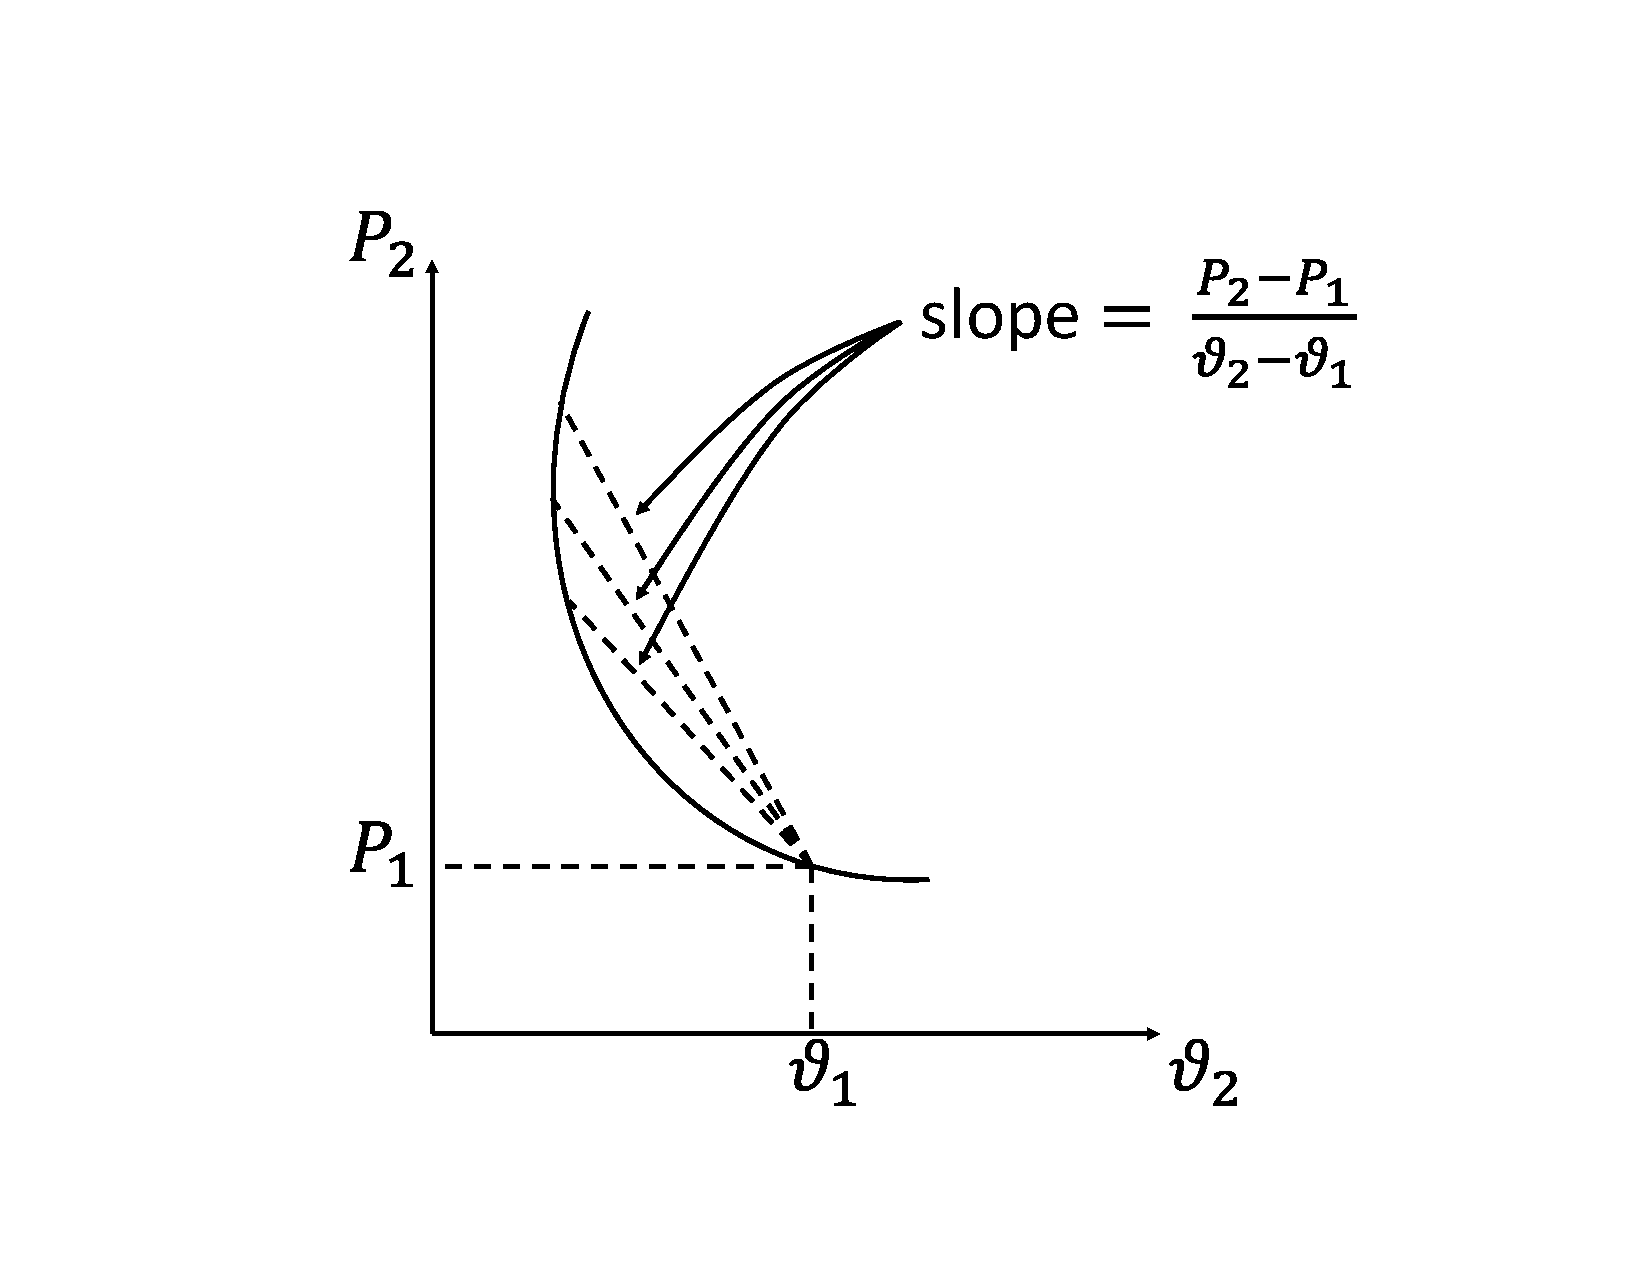
\includegraphics[width=0.7\textwidth]{../../images/shock_adiabat.pdf}
   \caption{Shock adiabat for an arbitrary equation of state.}
   \label{fig:shock_adiabat}
\end{figure}

A few extra notes on shock waves:
\begin{itemize}
    \item The shock Mach number $M_{1n}$ is defined as
    \begin{equation}
        M_{1n} = \frac{w_1}{c_1}.
    \end{equation}
    
    \item The speed of sound is independent of the reference frame. Thus, whether you are in the shock reference frame, or in a stationary reference frame, the speeds of sound before and after the shock are invariant.
    
    \item The relative velocities satisfy
    \begin{align}
        w_1 \ge &c_1 \nonumber \\
        w_2 \le &c_2.
    \end{align}
    
    \item The shock strength $\Pi$ is defined as (see \cite{thompson1988} for derivation):
    \begin{equation}
    \label{eq:shock_strength}
        \Pi = \frac{P_2 - P_1}{\rho_1 c_1^2}.
    \end{equation}
    
    \item Strong and weak shocks are defined according to
    \begin{align}
    \label{eq:strong_weak_shocks}
        \Pi \ll 1 \quad & \text{weak shock} \nonumber \\
        \Pi \gg 1 \quad & \text{strong shock}.
    \end{align}
    
    \item For weak shocks the entropy increase across a shock is so weak, they might as well be considered isentropic.
    
    \item In the limit of vanishing strength, shock waves become acoustic discontinuities, propagating with speed $c$ relative to the fluid.
\end{itemize}

%---------------------------------
\subsection{Normal shocks}
%---------------------------------
Following the derivations in \cite{thompson1988} for a perfect gas, one can express shock jump conditions as a function of $\gamma$ and $M_{1n}$ only. These are
\begin{equation}
\label{eq:normal_shock_pressure}
    \frac{P_2}{P_1} = \dfrac{\dfrac{2 \gamma}{\gamma - 1} M_{1n}^2 - 1}{\dfrac{\gamma + 1}{\gamma-1}},
\end{equation}
\begin{equation}
\label{eq:normal_shock_velocity}
    \frac{w_2}{w_1} = \dfrac{1 + \dfrac{\gamma - 1}{2} M_{1n}^2}{\dfrac{\gamma + 1}{2} M_{1n}^2},
\end{equation}
\begin{equation}
\label{eq:normal_shock_density}
    \frac{\rho_2}{\rho_1} = \dfrac{\dfrac{\gamma + 1}{2} M_{1n}^2}{1 + \dfrac{\gamma - 1}{2} M_{1n}^2}.
\end{equation}
Additionally, combining the three above one obtains
\begin{equation}
\label{eq:normal_shock_mach}
    M_{2n}^2 = \dfrac{M_{1n}^2 + \dfrac{2}{\gamma - 1}}{ \dfrac{2\gamma}{\gamma - 1}M_{1n}^2 - 1}.
\end{equation}

According to \cref{eq:shock_jump_energy} $h_{t2} = h_{t1}$ (this holds not only for normal shocks but all shocks). Thus, $T_{t2} = T_{t1}$. For the stagnation pressure, we have
\begin{equation}
\frac{P_{t2}}{P_{t1}} = \frac{P_{t2}}{P_2} \frac{P_1}{P_{t1}} \frac{P_2}{P_1}.
\end{equation}
Using \cref{eq:stagnation_pressure,eq:normal_shock_pressure,eq:normal_shock_mach}, and rearranging, one obtains
\begin{equation}
\label{eq:normal_shock_stagnation_pressure}
    \frac{P_{t2}}{P_{t1}} = \left ( \dfrac{ \dfrac{\gamma + 1}{\gamma - 1} }{ \dfrac{2 \gamma}{\gamma - 1} M_{1n}^2 - 1} \right) ^{ 1 / (\gamma - 1) } \left ( \dfrac{ \dfrac{\gamma + 1}{2} M_{1n}^2 }{ 1 + \dfrac{\gamma - 1}{2} M_{1n}^2 } \right ) ^{\gamma / (\gamma - 1)}.
\end{equation}
Finally, entropy change across a normal shock is
\begin{equation}
s_2 - s_1 = -R \ln \frac{P_{t2}}{P_{t1}},
\end{equation}
as shown in \cite{thompson1988}.

%---------------------------------
\subsection{Oblique shocks}
%---------------------------------
\begin{figure}[ht]
\centering
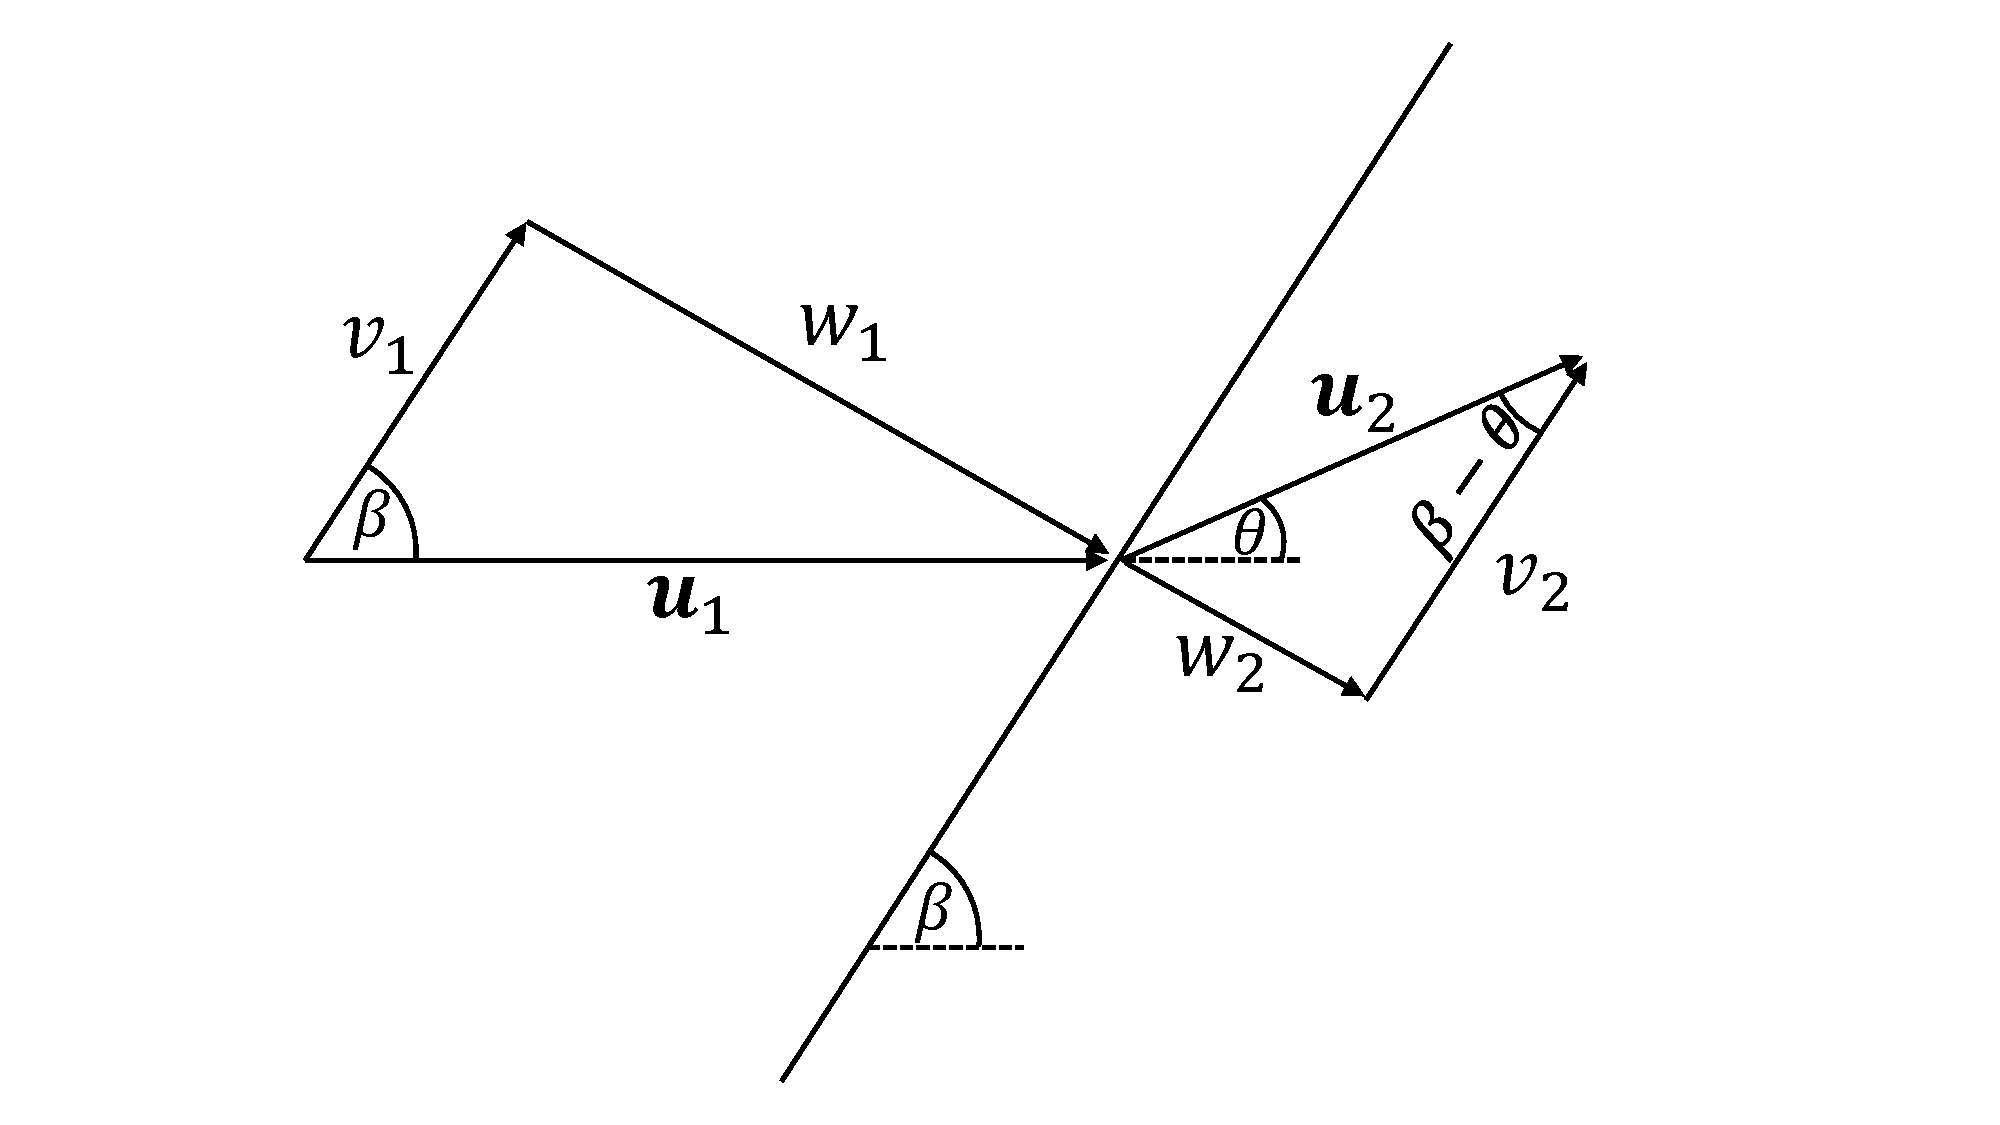
\includegraphics[width=10cm]{../../images/oblique_shock.pdf}
\caption{Oblique-shock geometry, $\beta$ is the shock angle and $\theta$ the turning angle.}
\label{fig:oblique_shock}
\end{figure}
The normal shock jump conditions given by \cref{eq:normal_shock_pressure,eq:normal_shock_velocity,eq:normal_shock_density,eq:normal_shock_mach,eq:normal_shock_stagnation_pressure} still apply, but it is again emphasized that $w_1$ and $w_2$ are the components normal to the shock, as defined in \cref{eq:shock_rel_vel_normal}. For the tangential components, defined by \cref{eq:shock_rel_vel_tangential}, we have $v_1 = v_2$ as mentioned in \cref{sec:shock_waves}. As shown in \cref{fig:oblique_shock}, the relationship between $w_1$, $w_2$ and $\uvec_1$, $\uvec_2$ is
\begin{align}
w_1 &= |\uvec_1| \sin{ \beta }, \nonumber \\
w_2 &= |\uvec_2| \sin( \beta - \theta ).
\end{align}
Similarly, the relationship between $v_1$, $v_2$ and $\uvec_1$, $\uvec_2$ is
\begin{align}
v_1 &= |\uvec_1| \cos{ \beta }, \nonumber \\
v_2 &= |\uvec_2| \cos (\beta - \theta).
\end{align}
If the upstream state is known ($\rho_1$, $\uvec_1$, $P_1$, $P_{t1}$), along with the shock angle $\beta$, then the downstream state can be determined using the above relationships and the normal shock jump conditions.

Using the shock jump condition for velocity (\cref{eq:normal_shock_velocity}), and some trigonometric identities, one can derive an equation for $\theta$ in terms of $\beta$, for a given inflow Mach number $M_1 = |\uvec_1|/c_1$, (see \cite{thompson1988}). This relationship is
\begin{equation}
    \tan \theta =\dfrac{ \cot \beta \left ( M_1^2 \sin^2 \beta - 1 \right ) }{ 1 + \left ( \frac{\gamma + 1}{2} \right ) M_1^2 - M_1^2 \sin^2 \beta}.
\end{equation}
The information contained in the above relationship is quite vast, and can best be understood by looking at $\theta$ profiles as a function of $\beta$---for different Mach numbers---obtained from the equation above. A plot of these profiles is given in \cref{fig:theta_beta_1}. Starting from the right-most point on the $x$-axis, labelled as ``a'', is a normal shock with a shock angle of $90^\circ$. Moving along the blue line as the shock angle decreases, we see that the turning angle increases until a maximum, labeled as ``b'', is reached. A further decrease in shock angle leads to point ``c'', which corresponds to turning angles for which the flow behind the shock becomes subsonic. Smaller shock angles lead to even smaller turning angles, until point ``d'' is reached, which corresponds to a Mach wave, to be described in a subsequent section. It is important to note that there are two shock angles that can give the same turning angle. The turning angle corresponding to the smaller shock angle is referred to as the weak solution, whereas the turning angle corresponding to the larger shock angle is the strong solution. This nomenclature has no direct connection to that defined in \cref{eq:strong_weak_shocks}. The black dashed line in \cref{fig:theta_beta_1} corresponds to the peak value for each Mach number, and thus demarcates the weak and strong solutions. A more pictorial representation of this behavior, for the specific case of a shock in front of a cylinder, is given in \cref{fig:theta_beta_2}. 
\begin{figure}[ht]
   \centering
   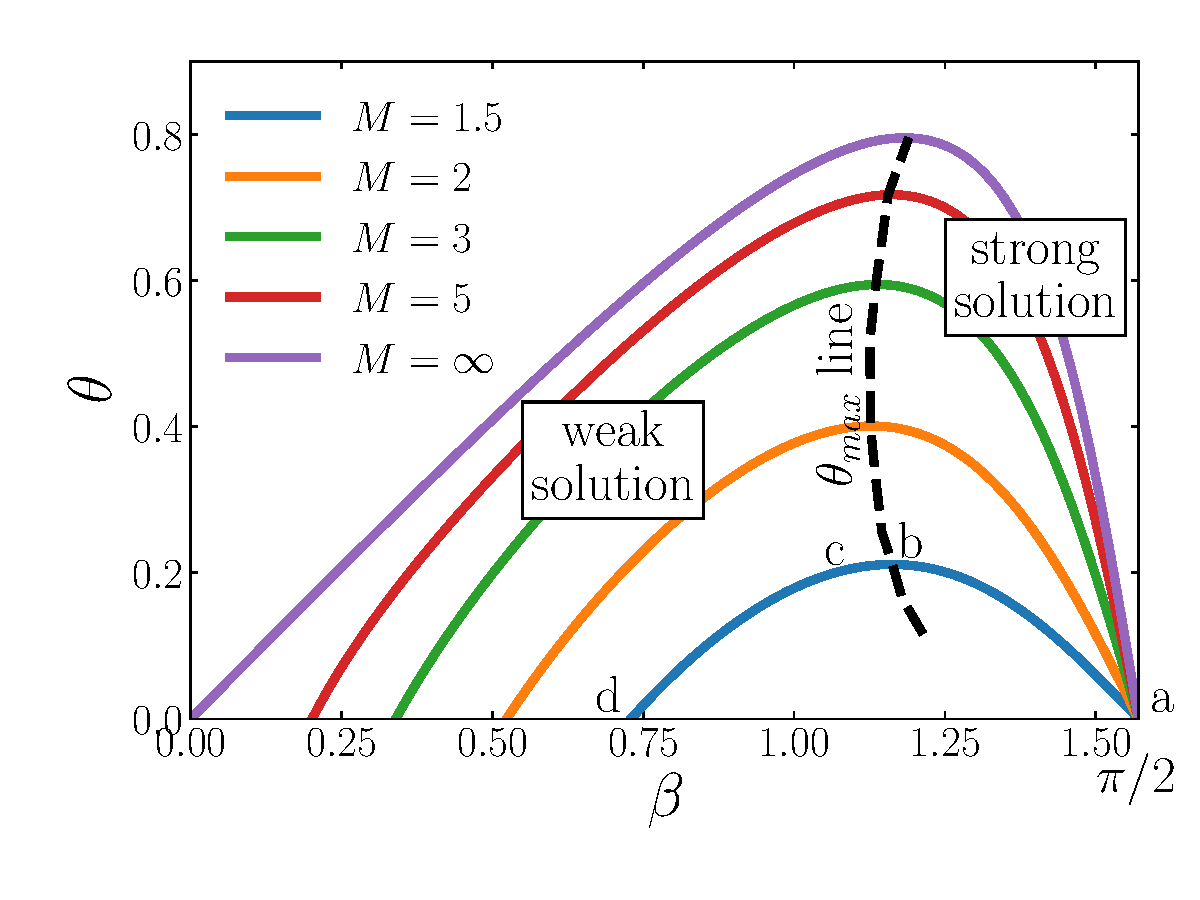
\includegraphics[width=0.5\textwidth]{../../images/theta_beta_1.pdf}
   \caption{$\theta$--$\beta$ curve for a perfect gas with $\gamma = 1.4$.}
   \label{fig:theta_beta_1}
\end{figure}

\begin{figure}[ht]
   \centering
   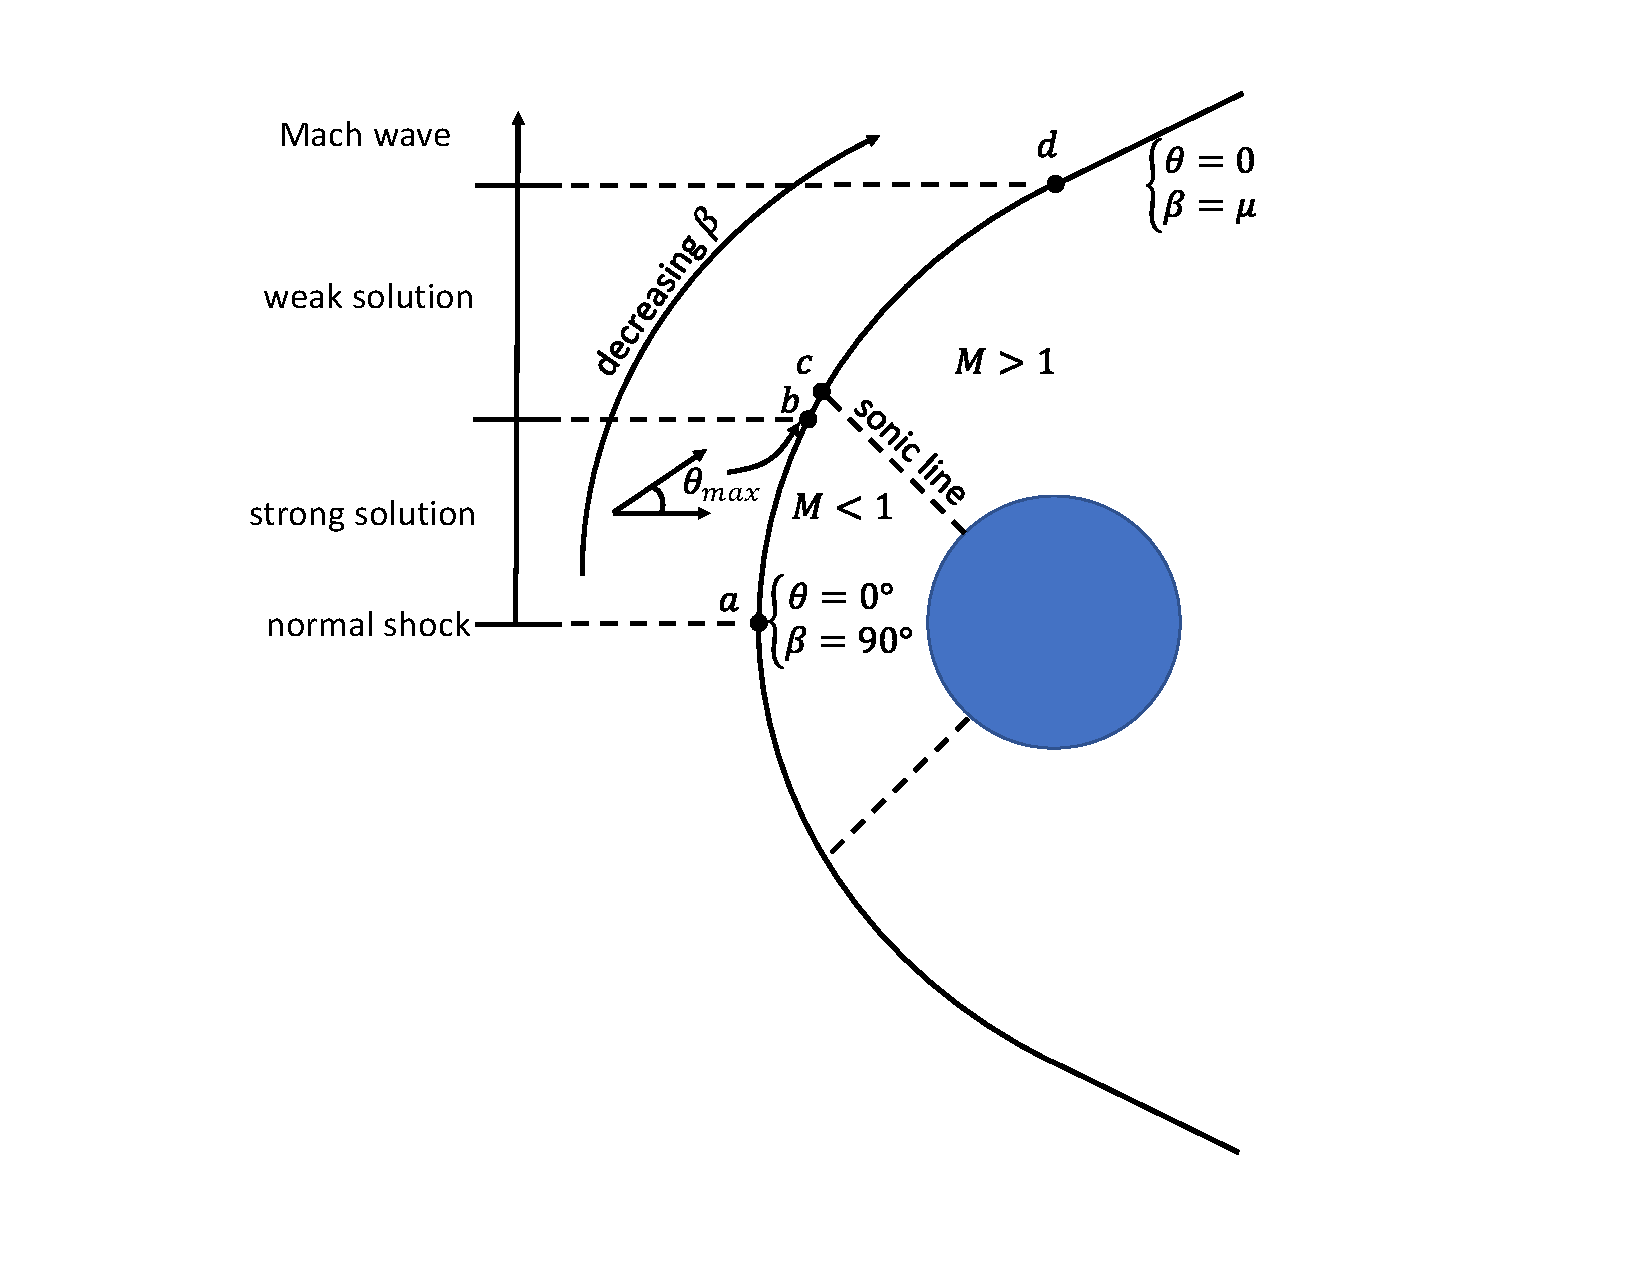
\includegraphics[width=0.7\textwidth]{../../images/theta_beta_2.pdf}
   \caption{Representation of different shock waves for different shock angles $\beta$.}
   \label{fig:theta_beta_2}
\end{figure}

Given the information above, it is relevant to ask what happens when a compressible fluid flows over a wedge or a some similar object, whose wedge angle is so large that the turning angle needs to be larger than $\theta_{max}$. Given that, as \cref{fig:theta_beta_1} shows, there is no turning angle greater than $\theta_{max}$, it seems like an inconsistency has been found. In reality, when the flow encounters a wedge whose angle is not that large and the turning angle can be lower than $\theta_{max}$, then the weak solution is the one that occurs and the shock is attached to the leading edge of the wedge. As the wedge angle increases and the flow needs to be deflected by an angle greater than $\theta_{max}$, the shock detaches from the wedge leading edge, as shown in \cref{fig:theta_beta_2}, and both strong and weak solutions occur along the shock. For this case, there will be a section behind the shock that will be subsonic, and thus the flow there can be turned by any angle greater than $\theta_{max}$.

%---------------------------------
\subsection{Weak shocks}
%---------------------------------
By definition, weak shocks are those for which $\Pi$, defined in \cref{eq:shock_strength}, is very small. Assuming that $\rho_1 c_1^2$ is not excessively large, the definition of $\Pi$ indicates that $P_2 - P_1$ is small for weak shocks. We can use the fact that $P_2 - P_1$ is small for weak shocks to show that $(s_2 - s_1) \propto (P_2-P_1)^3$, which then indicates weak shocks have negligible entropy changes.

We begin by adding and subtracting $(P_2 - P_1) \vartheta_1$ on the right-hand side of the Rankine-Hugoniot \cref{eq:rankine_hugoniot} to obtain
\begin{equation}
\label{eq:rankine_hugoniot_vartheta}
    h_2 - h_1 = (P_2 - P_1) \vartheta_1 + \frac{1}{2} (P_2 - P_1) (\vartheta_2 - \vartheta_1).
\end{equation}
We now use Taylor-series expansions for $h$ and $\vartheta$, each as a function of $s$ and $P$, and plug them into the equation above to obtain the scaling of $s$ as a function of $P$. For an arbitrary function $f(s,P)$ the Taylor-series expansion can symbolically be expressed as
\begin{align}
    f_2 - f_1 = &\left [ (s_2 - s_1) \left ( \frac{\partial}{\partial s} \right)_1 + (P_1 - P_1) \left( \frac{\partial}{\partial P} \right)_1 \right ] f \nonumber \\
    + \frac{1}{2! } &\left [ (s_2 - s_1) \left ( \frac{\partial}{\partial s} \right)_1 + (P_1 - P_1) \left( \frac{\partial}{\partial P} \right)_1 \right ]^2 f \nonumber \\
    + \frac{1}{3!}  &\left [ (s_2 - s_1) \left ( \frac{\partial}{\partial s} \right)_1 + (P_1 - P_1) \left( \frac{\partial}{\partial P} \right)_1 \right ]^3 f + ...\nonumber
\end{align}
Since we are interested in the leading-order expression for $(s_2 - s_1)$, terms of higher-order than $(s_2 - s_1)$ will be neglected, i.e. $(s_2 - s_1)^2$, $(s_2 - s_1)^3$, $(s_2 - s_1) (P_2 - P_1)$, etc. 

The Taylor-series expansion for enthalpy is
\begin{equation}
    h_2 - h_1 = (s_2 - s_1) \left ( \frac{\partial h}{\partial s} \right)_1 + (P_2 - P_1) \left ( \frac{\partial h}{\partial P} \right)_1 + \frac{1}{2} (P_2 - P_1)^2 \left( \frac{\partial^2 h}{\partial P^2} \right)_1 + \frac{1}{6}  (P_2 - P_1)^3 \left ( \frac{\partial^3 h}{\partial P^3} \right)_1 + ...
\end{equation}
Using the Gibbs equation shown in \cref{eq:gibbs_form_2}, we have $(\partial h / \partial s)_p = T$ and $(\partial h/ \partial P)_s = \vartheta$. Using this in the above gives
\begin{equation}
    h_2 - h_1 = (s_2 - s_1) T_1 + (P_2 - P_1) \vartheta_1 + \frac{1}{2} (P_2 - P_1)^2 \left( \frac{\partial \vartheta}{\partial P} \right)_1 + \frac{1}{6}  (P_2 - P_1)^3 \left ( \frac{\partial^2 \vartheta}{\partial P^2} \right)_1 + ...
\end{equation}
The Taylor-series expansion for the specific volume is
\begin{equation}
    \vartheta_2 - \vartheta_1 = (s_2 - s_1) \left ( \frac{\partial \vartheta}{\partial s} \right)_1 + (P_2 - P_1) \left ( \frac{\partial \vartheta}{\partial P} \right)_1 + \frac{1}{2} (P_2 - P_1)^2 \left( \frac{\partial^2 \vartheta}{\partial P^2} \right)_1 + \frac{1}{6}  (P_2 - P_1)^3 \left ( \frac{\partial^3 \vartheta}{\partial P^3} \right)_1 + ...    
\end{equation}
Plugging in the two Taylor-series expansions above in \cref{eq:rankine_hugoniot_vartheta}, gives
\begin{multline}
(s_2 - s_1) T_1 + (P_2 - P_1) \vartheta_1 + \frac{1}{2} (P_2 - P_1)^2 \left( \frac{\partial \vartheta}{\partial P} \right)_1 + \frac{1}{6}  (P_2 - P_1)^3 \left ( \frac{\partial^2 \vartheta}{\partial P^2} \right)_1 =\\
(P_2 - P_1) \vartheta_1 + \frac{1}{2} (P_2 - P_1)^2 \left ( \frac{\partial \vartheta}{\partial P} \right)_1 + \frac{1}{4} (P_2 - P_1)^3 \left ( \frac{\partial^2 \vartheta}{\partial P^2} \right)_1 + ...
\end{multline}
Simplifying the above finally gives
\begin{equation}
    s_2 - s_1 = \frac{1}{12 T_1} \left ( \frac{\partial^2 \vartheta}{\partial P^2} \right)_1 (P_2 - P_1)^3 + ...
\end{equation}
that is, $(s_2 - s_1) \propto (P_2-P_1)^3$.

%---------------------------------
\subsection{Strong shocks}
%---------------------------------
Strong shocks are defined as those for which $\Pi \gg 1$. In general, it seems that $P < \rho c^2$, and thus
\begin{equation}
    \Pi =  \frac{P_2}{\rho_1 c_1^2} - \frac{P_1}{\rho_1 c_1^2} \gg 1
\end{equation}
becomes
\begin{equation}
    \frac{P_2}{\rho_1 c_1^2}  \gg 1,
\end{equation}
or
\begin{equation}
    P_2 \gg \rho_1 c_1^2.
\end{equation}
The above in turn implies $P_2 \gg P_1$, that is, $P_1$ is negligible.

Consider the normal shock jump condition for pressure given by \cref{eq:normal_shock_pressure}. It can be rearranged to give
\begin{equation}
P_2 = \dfrac{ \dfrac{2 \gamma}{\gamma - 1} \dfrac{\rho_1 w_1^2}{\gamma} - P_1}{\dfrac{\gamma + 1}{\gamma - 1}}.
\end{equation}
Since $P_1$ can be neglected, this gives
\begin{equation}
\label{eq:normal_shock_pressure_strong}
    P_2 = \frac{2}{\gamma + 1} \rho_1 w_1^2.
\end{equation}
Additionally, since $M_{1n}^2 = \rho_1 w_1^2 / \gamma P_1$, a negligible $P_1$ leads to $M_{1n}^2 \gg 1$. Thus, \cref{eq:normal_shock_velocity,eq:normal_shock_density,eq:normal_shock_mach} give
\begin{equation}
\label{eq:normal_shock_velocity_strong}
    \frac{w_2}{w_1} = \frac{\gamma -1}{\gamma + 1},
\end{equation}
\begin{equation}
\label{eq:normal_shock_density_strong}
    \frac{\rho_2}{\rho_1} = \frac{\gamma + 1}{\gamma -1},
\end{equation}
and
\begin{equation}
\label{eq:normal_shock_mach_strong}
    M_{2n}^2 = \frac{\gamma - 1}{2\gamma}.
\end{equation}


%------------------------------------------------------------------------
\section{Mach Waves}
%------------------------------------------------------------------------

\begin{figure}[ht]
\centering
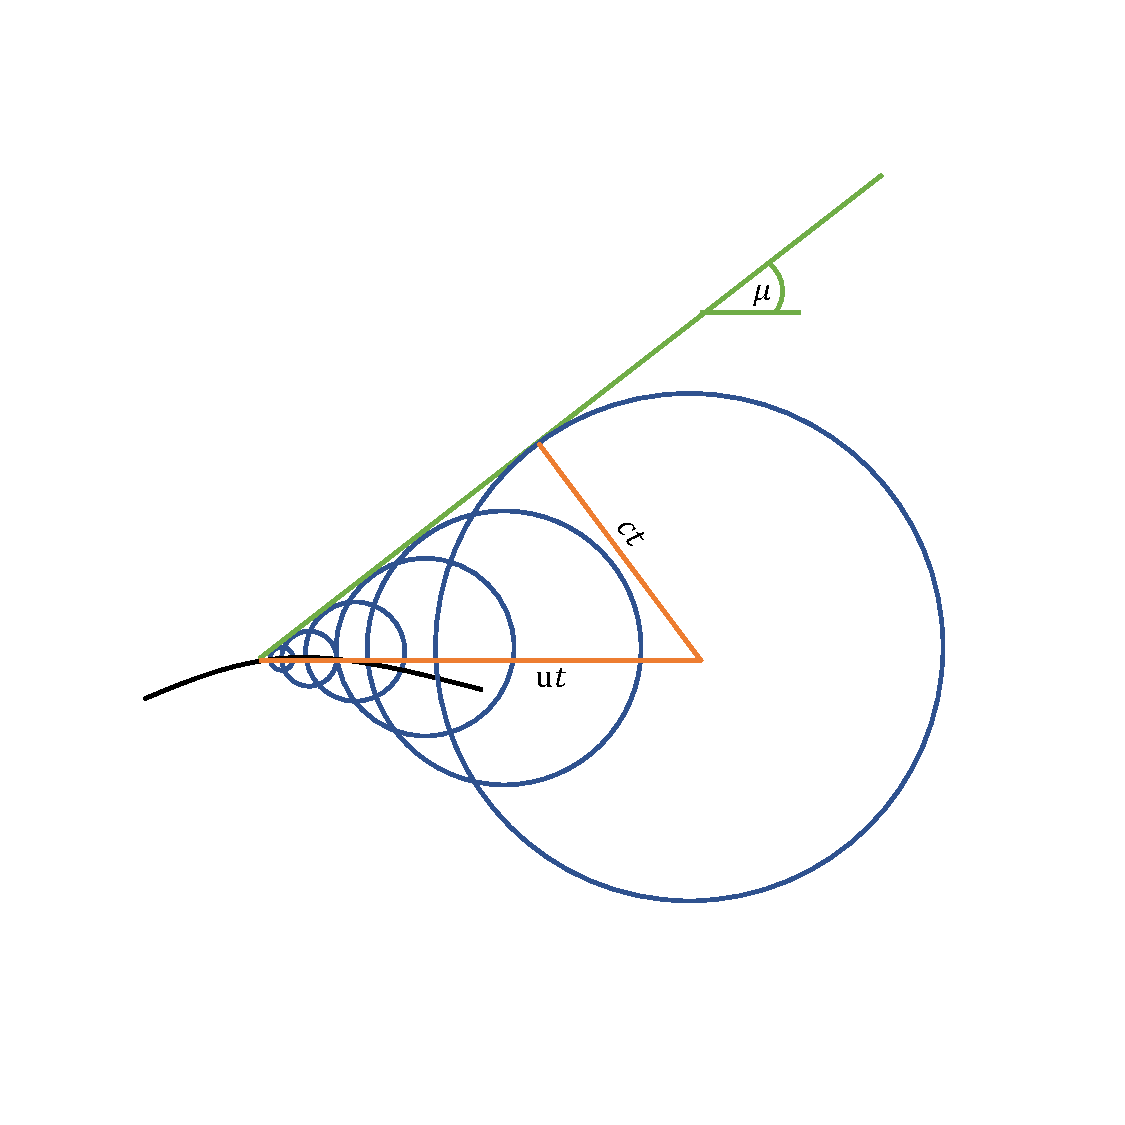
\includegraphics[width=8cm]{../../images/mach_wave.pdf}
\caption{Mach wave}
\label{fig:mach_wave}
\end{figure}
Assume a vehicle is moving at a Mach number greater than one. In \cref{fig:mach_wave}, the black line represents a section of the surface of the vehicle moving at supersonic speeds. At each instance in time, each infinitesimal point on this surface slightly distorts the stationary fluid and thus produces acoustic waves (blue line). These waves, by definition, expand at the speed of sound. The green line, which is aligned with the front of the acoustic waves, is referred to as a Mach wave or Mach line. The angle of inclination of this Mach wave, labeled $\mu$, is called the Mach angle and satisfies
\begin{equation}
    \sin (\mu) = \frac{1}{M}.
\end{equation}


%------------------------------------------------------------------------
\section{Contact discontinuities}
%------------------------------------------------------------------------
A contact discontinuity is defined as a surface that separates two fluids of different properties or at different states. A defining condition is that there is no flow of matter across a contact discontinuity, that is, $w_1 = w_2 = 0$. Using this in the integral momentum conservation equation for a thin box bounding the discontinuity, and assuming negligible viscous stresses and heat fluxes, leads to $P_1 = P_2$. However, other flow properties, such as $\rho$, $T$, and $v$ can change across the discontinuity.

%########################################################################
\chapter{Quasi 1-D steady and unsteady flow}
%########################################################################
Quasi 1-D eqs; mass balance, f(M), and PAFMT; Fanno flow, Rayleigh flow.

%########################################################################
Local acoustic speed, Expansion and Compression wave, Shock tube.

%########################################################################
\chapter{2-D Compressible flow}
%########################################################################
Prandtl-Meyer (Compressive, Expansive); Shock-Expansion Theory: 2D Airfoil Calculations, Shock Reflection, Isentropic flow in curved channel, Nozzle exit flows.

%%%%%%%%%%%%%%%%%%%%%%%%%%%%%%%%%%%%%%%%%%%%%%%%%%%%%%%%%%%%%%%%%%%%%%%%%
\part{Viscous Flow}
%%%%%%%%%%%%%%%%%%%%%%%%%%%%%%%%%%%%%%%%%%%%%%%%%%%%%%%%%%%%%%%%%%%%%%%%%

%########################################################################
\chapter{Viscous solutions of the Navier Stokes Equations}
%########################################################################
Viscous effects include friction drag, flow separation(leading edge stall, trailing edge stall, thin airfoil stall), and viscous dissipation.

%------------------------------------------------------------------------
\section{Steady Parallel Flows}
%------------------------------------------------------------------------

%---------------------------------
\subsection{Couette flow} 
%---------------------------------

%---------------------------------
\subsection{Poiseuille flow (plane and circular)}
%---------------------------------

%---------------------------------
\subsection{Combined Couette and Poiseuille flow}
%---------------------------------

%------------------------------------------------------------------------
\section{Unsteady Parallel Flows}
%------------------------------------------------------------------------

%---------------------------------
\subsection{Stokes first problem}
%---------------------------------

%---------------------------------
\subsection{Stokes second problem}
%---------------------------------

%------------------------------------------------------------------------
\section{Lubrication Theory and Flow in thin structures}
%------------------------------------------------------------------------

%########################################################################
\chapter{Boundary Layers}
%########################################################################

%------------------------------------------------------------------------
\section{Introduction}
%------------------------------------------------------------------------

%---------------------------------
\subsection{Scaling of boundary layer thickness}
%---------------------------------

%---------------------------------
\subsection{B.L. eqs. as result of non-dimensionalization of NS eqs.}
%---------------------------------

%---------------------------------
\subsection{Displacement thickness (different interpretations), Momentum thickness}
%---------------------------------

%---------------------------------
\subsection{Iterative procedure for coupled viscous-inviscid solution.}
%---------------------------------

%------------------------------------------------------------------------
\section{Integral Methods}
%------------------------------------------------------------------------

%---------------------------------
\subsection{Von Karman Momentum Integral Equation}
%---------------------------------

%---------------------------------
\subsection{Pohlhausen}
%---------------------------------

%---------------------------------
\subsection{Thwaites}
%---------------------------------

%------------------------------------------------------------------------
\section{Exact Solutions}
%------------------------------------------------------------------------

%---------------------------------
\subsection{Blasius}
%---------------------------------

%---------------------------------
\subsection{Falkner Skan}
%---------------------------------

%%%%%%%%%%%%%%%%%%%%%%%%%%%%%%%%%%%%%%%%%%%%%%%%%%%%%%%%%%%%%%%%%%%%%%%%%
\part{Hydrodynamic Instabilities}
%%%%%%%%%%%%%%%%%%%%%%%%%%%%%%%%%%%%%%%%%%%%%%%%%%%%%%%%%%%%%%%%%%%%%%%%%

%########################################################################
\chapter{Hydrodynamic Instabilities}
%########################################################################

%------------------------------------------------------------------------
\section{Linear Stability}
%------------------------------------------------------------------------
Consider the following system of PDEs for a two-dimensional problem
\begin{equation}
    \frac{\partial w}{\partial t} = \frac{\partial \phi}{\partial y}\frac{\partial w}{\partial x} - \frac{\partial \phi}{\partial x} \frac{\partial w}{\partial y},
\end{equation}
\begin{equation}
    w = \nabla^2 \phi .
\end{equation}
In the above, $\phi = \phi(x,y,t)$ is the electrostatic potential and $w = w(x,y,t)$ the vorticity.

The analysis begins by splitting the variables into equilibrium and fluctuating components, namely
\begin{equation}
    \phi = \phi_0 + \phi_1,
\end{equation}
\begin{equation}
    w = w_0 + w_1.
\end{equation}
For the above, $\phi_0 = \phi_0(x)$, $w_0 = w_0(x)$, and $\phi_1 = \phi_1(x,y,t)$, $w_1 = w_1(x,y,t)$. We now introduce a Fourier series decomposition for the fluctuating variables, and focus on a single Fourier mode as follows 
\begin{equation}
    \phi_1(x,y,t) = F(x,k_y,t) e^{ik_y y} = \tilde{\phi}(x,k_y) e^{\gamma t + i k_y y},
\end{equation}
\begin{equation}
    w_1(x,y,t) = G(x,k_y,t) e^{ik_y y} = \tilde{w}(x,k_y) e^{\gamma t + i k_y y}.
\end{equation}
In the above, $\gamma$, which can be complex, is the growth rate factor, and $\tilde{\phi} = \tilde{\phi}(x, k_y)$, $\tilde{w} = \tilde{w}(x, k_y)$ are the remaining part of the Fourier coefficient.

We then plug in the decompositions for $\phi$ and $w$ in the governing PDEs. Collecting the lowest order terms leads to equations for the equilibrium solution. For example, the Poisson equation to lowest order is
\begin{equation}
    \label{eq:lin_stab_w0_phi0}
    w_0 = \nabla^2 \phi_0 = \frac{\partial^2 \phi_0}{\partial x^2}.
\end{equation}
Combining terms up to next order gives
\begin{equation}
    \label{eq:lin_stab_pde_mid_order}
    \frac{\partial w_1}{\partial t} = \frac{\partial \phi_0}{\partial y}\frac{\partial w_1}{\partial x} + \frac{\partial \phi_1}{\partial y}\frac{\partial w_0}{\partial x} - \frac{\partial \phi_0}{\partial x} \frac{\partial w_1}{\partial y} - \frac{\partial \phi_1}{\partial x} \frac{\partial w_0}{\partial y},
\end{equation}
\begin{equation}
    w_1 = \nabla^2 \phi_1.
\end{equation}
Using the expression for $\phi_1$ in the Poisson equation above leads to 
\begin{equation}
    w_1 = \left ( \frac{\partial^2 \tilde{\phi}}{\partial x^2} - k_y^2 \tilde{\phi} \right ) e^{\gamma t + i k_y y},
\end{equation}
or 
\begin{equation}
    \tilde{w} = \frac{\partial^2 \tilde{\phi}}{\partial x^2} - k_y^2 \tilde{\phi} .
\end{equation}
We'll now evaluate each of the terms in \cref{eq:lin_stab_pde_mid_order}.
\begin{align}
    \frac{\partial w_1}{\partial t} &= \gamma \left ( \frac{\partial^2 \tilde{\phi}}{\partial x^2} - k_y^2 \tilde{\phi} \right ) e^{\gamma t + i k_y y}, \nonumber \\
    \frac{\partial \phi_0}{\partial y}\frac{\partial w_1}{\partial x} &= 0, \nonumber \\
    \frac{\partial \phi_1}{\partial y}\frac{\partial w_0}{\partial x} &= i k_y \tilde{\phi} e^{\gamma t + i k_y y} \frac{\partial^3 \phi_0}{\partial x^3}, \nonumber \\
    \frac{\partial \phi_0}{\partial x} \frac{\partial w_1}{\partial y} &= \frac{\partial \phi_0}{\partial x} i k_y \left ( \frac{\partial^2 \tilde{\phi}}{\partial x^2} - k_y^2 \tilde{\phi} \right ) e^{\gamma t + i k_y y},\nonumber \\
    \frac{\partial \phi_1}{\partial x} \frac{\partial w_0}{\partial y} &= 0 . \nonumber \\
\end{align}
Combining all of the above, we obtain
\begin{equation}
    \gamma \left ( \frac{\partial^2 \tilde{\phi}}{\partial x^2} - k_y^2 \tilde{\phi} \right ) = ik_y \tilde{\phi} \frac{\partial^3 \phi_0}{\partial x^3} - \frac{\partial \phi_0}{\partial x} i k_y \left ( \frac{\partial^2 \tilde{\phi}}{\partial x^2} - k_y^2 \tilde{\phi} \right ).
\end{equation}
This is re-written as 
\begin{equation}
    \gamma \left ( \frac{\partial^2 \tilde{\phi}}{\partial x^2} - k_y^2 \tilde{\phi} \right ) = -i k_y \left [ \frac{\partial \phi_0}{\partial x} \left ( \frac{\partial^2 \tilde{\phi}}{\partial x^2} - k_y^2 \tilde{\phi} \right ) - \frac{\partial^3 \phi_0}{\partial x^3} \tilde{\phi} \right ].
\end{equation}

%%%%%%%%%%%%%%%%%%%%%%%%%%%%%%%%%%%%%%%%%%%%%%%%%%%%%%%%%%%%%%%%%%%%%%%%%
\appendix
%%%%%%%%%%%%%%%%%%%%%%%%%%%%%%%%%%%%%%%%%%%%%%%%%%%%%%%%%%%%%%%%%%%%%%%%%

%########################################################################
\chapter{Vectors in rotating reference frames}
%########################################################################

%------------------------------------------------------------------------
\section{Basic properties}
%------------------------------------------------------------------------

%--------------------------------------------
\subsection{Position}
%--------------------------------------------
Consider the Euclidean transformation
\begin{equation}
\label{eq:x_rot}
\tilde{x}^+_i(\tilde{t}) = Q_{ij}(\tilde{t}-c) x^+_j(\tilde{t}-c) + b_i(\tilde{t}-c) 
\end{equation}
where $x^+(t)$ is the Lagrangian position of a fluid particle, and $\tilde{x}^+(\tilde{t})$ is the Lagrangian position of the same particle but in a rotating reference frame. The transformation above amounts to a rotation of the reference frame determined by the orthogonal matrix $\mathbf{Q}(t)$, a translation of the reference frame determined by the vector $\mathbf{b}(t)$, and a translation in time given by $\tilde{t} = t + c$. 

%--------------------------------------------
\subsection{Velocity}
%--------------------------------------------
Since the velocity of a fluid particle is given by 
\begin{equation}
u^+_i(t) = \frac{d x^+_i(t)}{dt},
\end{equation}
the components of velocity in the non-inertial reference frame are defined as
\begin{equation}
\tilde{u}^+_i(\tilde{t}) = \frac{d \tilde{x}^+_i(\tilde{t})}{d \tilde{t}} .
\end{equation}
Thus, the relationship between the velocity components in the different reference frames is given by
\begin{align}
\label{eq:rot_vel_general}
\tilde{u}^+_i(\tilde{t}) &= \frac{d}{d\tilde{t}} [Q_{ij}(\tilde{t} - c) x^+_j(\tilde{t} - c) + b_i(\tilde{t} - c)] \nonumber \\
& = Q_{ij}(\tilde{t} - c) U^+_j(\tilde{t} - c) + \dot{Q}_{ij}(\tilde{t} - c) x^+_j(\tilde{t} - c) + \dot{b}_i(\tilde{t} - c).
\end{align}
If we assume there is no translation in space or time, the above reduces to
\begin{equation}
\label{eq:rot_vel_inter}
\tilde{u}^+_i = Q_{ij} u^+_j + \dot{Q}_{ij} x^+_j, 
\end{equation}
where each quantity above depends on time $t$. Multiplying by $Q^{-1}_{ki}$ we obtain
\begin{equation}
Q_{ik} \tilde{u}^+_i = u^+_k + Q_{ik}\dot{Q}_{ij}x^+_j.
\end{equation}
Noting that the tensor $Q_{ik} \dot{Q}_{ij}$ is antisymmetric, we obtain
\begin{equation}
\label{eq:rot_vel}
u^+_k = Q_{ik} \tilde{u}^+_i + Q_{ij}\dot{Q}_{ik}x^+_j.
\end{equation}

We now define the angular velocity tensor $\Omega_{ij}$ and the angular velocity vector $\Omega_i$ using the following relationship 
\begin{equation}
\label{eq:angular_definition}
\Omega_{ij} = \epsilon_{jik}\Omega_{k} = Q_{kj}\dot{Q}_{ki}.
\end{equation}
Thus (\ref{eq:rot_vel}) can be expressed in terms of the angular velocity tensor as
\begin{equation}
\label{eq:rot_vel_angular_tensor}
u^+_k = Q_{ik} \tilde{u}^+_i + \Omega_{kj}x^+_j,
\end{equation}
or in terms of the angular velocity vector as
\begin{equation}
\label{rot_vel_angular_vector}
u^+_k = Q_{ik} \tilde{u}^+_i + \epsilon_{jki}\Omega_ix^+_j.
\end{equation}

%--------------------------------------------
\subsection{Acceleration}
%--------------------------------------------
We assume again no translation in space or time. Taking the derivative of both sides of \cref{eq:rot_vel}
\begin{equation}
    \frac{du^+_k}{dt} = \dot{Q}_{ik} \tilde{u}^+_i + Q_{ik} \frac{d\tilde{u}^+_i}{dt} + \dot{Q}_{ik} \frac{dQ_{ij} x^+_j}{dt} + Q_{ij}\ddot{Q}_{ik} x^+_j.
\end{equation}
Using \cref{eq:x_rot} the above is re-written as
\begin{equation}
    \frac{du^+_k}{dt} = Q_{ik} \frac{d\tilde{u}^+_i}{dt} + 2 \dot{Q}_{ik} \tilde{u}^+_i + Q_{ij}\ddot{Q}_{ik} x^+_j.
\end{equation}
Re-writing the last term on the right-hand-side above leads to
\begin{equation}
    \frac{du^+_k}{dt} = Q_{ik} \frac{d\tilde{u}^+_i}{dt} + 2 \dot{Q}_{ik} \tilde{u}^+_i + \frac{d Q_{ij}\dot{Q}_{ik}}{dt} x^+_j - \dot{Q}_{ij} \dot{Q}_{ik} x^+_j.
\end{equation}
We now show that
\begin{align}
    \dot{Q}_{ij} \dot{Q}_{ik} & = \delta_{pi}\dot{Q}_{pj} \dot{Q}_{ik}  \nonumber \\
    & = Q_{pq}Q^{-1}_{qi} \dot{Q}_{pj} \dot{Q}_{ik}  \nonumber \\
    & = Q_{pq} \dot{Q}_{pj} Q_{iq} \dot{Q}_{ik} .
\end{align}
Thus, in terms of the angular velocity tensor, we have
\begin{equation}
    \frac{du^+_k}{dt} = Q_{ik} \frac{d\tilde{u}^+_i}{dt} + 2 \dot{Q}_{ik} \tilde{u}^+_i + \frac{d \Omega_{kj}}{dt} x^+_j - \Omega_{kq} \Omega_{jq} x^+_j.
\end{equation}
In terms of the angular velocity vector, the above becomes
\begin{equation}
    \frac{du^+_k}{dt} = Q_{ik} \frac{d\tilde{u}^+_i}{dt} + 2 \dot{Q}_{ik} \tilde{u}^+_i + \epsilon_{jki}\frac{d \Omega_{i}}{dt} x^+_j - \epsilon_{qki}\Omega_{i} \epsilon_{qjp}\Omega_{p} x^+_j,
\end{equation}
which, upon a simple re-arrangement of indices, gives
\begin{equation}
\label{eq:rot_acl_angular_vector}
    \frac{du^+_k}{dt} = Q_{ik} \frac{d\tilde{u}^+_i}{dt} + 2 \dot{Q}_{ik} \tilde{u}^+_i + \epsilon_{kij}\frac{d \Omega_{i}}{dt} x^+_j + \epsilon_{kiq}\Omega_{i} \epsilon_{qpj}\Omega_{p} x^+_j.
\end{equation}

%------------------------------------------------------------------------
\section{Unit vectors}
%------------------------------------------------------------------------
Let the orthogonal basis for the inertial reference frame be denoted by $\hat{a}^{(1)}$, $\hat{a}^{(2)}$, and $\hat{a}^{(3)}$, and the orthogonal basis for the rotating reference frame by $\hat{b}^{(1)}$, $\hat{b}^{(2)}$, and $\hat{b}^{(3)}$. We know that the unit vector $\hat{b}^{(i)}$ has components $\tilde{b}_j^{(i)}$ in the rotating reference frame, and components $b_j^{(i)}$ in the inertial reference frame. The vector is the same whether expressed in the rotating or inertial reference frames, that is
\begin{equation}
\tilde{b}_k^{(i)} \hat{b}^{(k)} = b_k^{(i)} \hat{a}^{(k)}
\end{equation}
Since $\tilde{b}_k^{(i)} = \delta_{ik}$, we rewrite the above as
\begin{equation}
\label{eq:unit_trans}
\hat{b}^{(i)} = b_k^{(i)} \hat{a}^{(k)} = Q_{jk} \tilde{b}_j^{(i)} \hat{a}^{(k)} = Q_{ik} \hat{a}^{(k)}.
\end{equation}
Doting both sides by $\hat{a}^{(j)}$ shows that 
\begin{equation}
Q_{ij} = \hat{a}^{(j)} \cdot \hat{b}^{(i)}.
\end{equation}

One can also multiply both sides of \cref{rot_vel_angular_vector} by $\hat{a}^{(k)}$ and use \cref{eq:unit_trans} to obtain
\begin{equation}
    \label{eq:uine_urot_temp}
u^+_k \hat{a}^{(k)} = \tilde{u}^+_i \hat{b}^{(i)} + \epsilon_{jki}\Omega_ix^+_j \hat{a}^{(k)}.
\end{equation}
If we introduce the following notation
\begin{align}
    \vec{u}^+_{ine} &= u^+_k \hat{a}^{(k)}, \\
    \vec{u}^+_{rot} &= \tilde{u}^+_i \hat{b}^{(i)}, \\
    \vec{\Omega} &= \Omega_i \hat{a}^{(i)}, \\
    \vec{x}^+ &= x_i^+ \hat{a}^{(i)}.
\end{align}
then the \cref{eq:uine_urot_temp} is written as 
\begin{equation}
\label{uine_urot}
\vec{u}^+_{ine}  = \vec{u}^+_{rot}  + \vec{\Omega} \times \vec{x}^+.
\end{equation}
Similarly, multiplying both sides of \cref{eq:rot_acl_angular_vector} gives
\begin{equation}
\label{eq:aine_arot_inter}
    \frac{du^+_k}{dt} \hat{a}^{(k)} = \frac{d\tilde{u}^+_i}{dt}\hat{b}^{(i)} + 2 \dot{Q}_{ik} \tilde{u}^+_i \hat{a}^{(k)} + \epsilon_{kij}\frac{d \Omega_{i}}{dt} x^+_j \hat{a}^{(k)} + \epsilon_{kiq}\Omega_{i} \epsilon_{qpj}\Omega_{p} x^+_j \hat{a}^{(k)}.
\end{equation}
Using \cref{eq:angular_definition} one can show that $\dot{Q}_{ik} = \epsilon_{pjk} \Omega_p Q_{ij}$. Thus, the second term on the left-hand-side above can be written as
\begin{align}
    2 \dot{Q}_{ik} \tilde{u}^+_i \hat{a}^{(k)} &= 2 \epsilon_{pjk} \Omega_p Q_{ij} \tilde{u}^+_i \hat{a}^{(k)} \nonumber \\
    &= 2 \Omega_p Q_{ij} \tilde{u}^+_i \hat{a}^{(p)} \times \hat{a}^{(j)} \nonumber \\
    &= 2 \Omega_p \hat{a}^{(p)} \times \tilde{u}^+_i \hat{b}^{(i)}.
\end{align}
Therefore, in vector notation \cref{eq:aine_arot_inter} becomes
\begin{equation}
    \label{eq:aine_arot}
    \vec{a}^+_{ine} = \vec{a}^+_{rot} + 2 \vec{\Omega} \times \vec{u}^+_{rot} + \dot{\vec{\Omega}} \times \vec{x}^+ + \vec{\Omega} \times (\vec{\Omega} \times \vec{x}^+),
\end{equation}
where $\vec{a}^+_{ine} = \frac{du^+_k}{dt} \hat{a}^{(k)}$, $\vec{a}^+_{rot} = \frac{d\tilde{u}^+_i}{dt}\hat{b}^{(i)}$, and $\dot{\vec{\Omega}} = \frac{d\Omega_i}{dt} \hat{a}^{(i)}$.

%------------------------------------------------------------------------
\section{Eulerian variables}
%------------------------------------------------------------------------
We now introduce the Eulerian counterpart to the Lagrangian variables. In the inertial reference frame these are $\rho(t,\xvec)$, $u_i(t,\xvec)$, and $p(t,\xvec)$. They are defined by the following expressions
\begin{align}
    \rho^+ &= \rho(t,\xvec^+) \\
    u_i^+ &= u_i(t,\xvec^+) \\
    p^+ &= p(t,\xvec^+).
\end{align}
Similarly for the rotating reference frame, we have $\tilde{\rho}(t,\tilde{\xvec})$, $\tilde{u}_i(t,\tilde{\xvec})$, and $\tilde{p}(t,\tilde{\xvec})$. These are defined by
\begin{align}
    \tilde{\rho}^+ &= \tilde{\rho}(t,\tilde{\xvec}^+) \\
    \tilde{u}_i^+ &= \tilde{u}_i(t,\tilde{\xvec}^+) \\
    \tilde{p}^+ &= \tilde{p}(t,\tilde{\xvec}^+).
\end{align}
We now use the transformation rules for the Lagrangian variables to derive the transformation rules for the Eulerian variables. The transformation rules for the Lagrangian variables are
\begin{align}
    \rho^+ &= \tilde{\rho}^+ \\
    u_k^+ &= Q_{ik} \tilde{u}_i^+ + Q_{ij} \dot{Q}_{ik} x_j^+ \\
    p^+ &= \tilde{p}^+.
\end{align}
The second equation above is the previously derived \cref{eq:rot_vel}. Using the definition of the Eulerian variables, the above is re-written as
\begin{align}
    \rho(t,\xvec^+) &= \tilde{\rho}(t,\tilde{\xvec}^+) \label{eq:eul_rho_temp} \\
    u_i(t,\xvec^+) &= Q_{ik} \tilde{u}_i(t,\tilde{\xvec}^+)  + Q_{ij} \dot{Q}_{ik} x_j^+ \label{eq:eul_vel_temp}\\
    p(t,\xvec^+) &= \tilde{p}(t,\tilde{\xvec}^+). \label{eq:pres_temp}
\end{align}
Using \cref{eq:x_rot}, we get
\begin{align}
    \rho(t,\xvec^+) &= \tilde{\rho}(t,\Qvec \xvec^+) \\
    u_i(t,\xvec^+) &= Q_{ik} \tilde{u}_i(t,\Qvec \xvec^+)  + Q_{ij} \dot{Q}_{ik} x_j^+ \\
    p(t,\xvec^+) &= \tilde{p}(t,\Qvec \xvec^+)+.
\end{align}
Since the above holds for any $\xvec^+$, we finally re-write it as
\begin{align}
    \rho(t,\xvec) &= \tilde{\rho}(t,\Qvec \xvec) \label{eq:eul_rho_trans}\\
    u_i(t,\xvec) &= Q_{ik} \tilde{u}_i(t,\Qvec \xvec)  + Q_{ij} \dot{Q}_{ik} x_j \label{eq:eul_vel_trans}\\
    p(t,\xvec) &= \tilde{p}(t,\Qvec \xvec). \label{eq:eul_pres_trans}
\end{align}

%------------------------------------------------------------------------
\section{Rotating Navier-Stokes equations}
%------------------------------------------------------------------------
We first obtain a few set of relationships that will later be used in deriving the rotating Navier-Stokes equations. Taking the derivative of \cref{eq:eul_pres_trans} gives
\begin{align}
    \frac{\partial p(t,\xvec)}{\partial x_i} &= \frac{ \partial \tilde{p}(t,\Qvec \xvec)}{\partial x_i} \nonumber \\
    &= \frac{\partial}{\partial x_i} \tilde{p}(t,Q_{1j}x_j, Q_{2j}x_j, Q_{3j} x_3) \nonumber \\
    &= \frac{\partial Q_{1j}x_j}{\partial x_i} \left [ \frac{\partial \tilde{p}(t,\tilde{\xvec})}{\partial \tilde{x}_1} \right]_{ \tilde{\xvec} = \Qvec \xvec} + \frac{\partial Q_{2j}x_j}{\partial x_i} \left [ \frac{\partial \tilde{p}(t,\tilde{\xvec})}{\partial \tilde{x}_2} \right ]_{\tilde{\xvec} = \Qvec \xvec} + \frac{\partial Q_{3j}x_j}{\partial x_i} \left [ \frac{\partial \tilde{p}(t,\tilde{\xvec})}{\partial \tilde{x}_3} \right ]_{\tilde{\xvec} = \Qvec \xvec} \nonumber \\
    &= Q_{ji} \left [ \frac{\partial \tilde{p}(t,\tilde{\xvec})}{\partial \tilde{x}_j} \right ]_{\tilde{\xvec} = \Qvec \xvec}
\end{align}
If we evaluate the above at $\xvec = \xvec^+$, we get
\begin{equation}
    \left [ \frac{\partial p(t,\xvec)}{\partial x_i} \right]_{\xvec = \xvec^+} = Q_{ji} \left [ \frac{\partial \tilde{p}(t,\tilde{\xvec})}{\partial \tilde{x}_j} \right]_{\tilde{\xvec} = \tilde{\xvec}^+}.
\end{equation}
Multiplying both sides by $\hat{a}^{(i)}$ gives
\begin{equation}
\label{eq:ns_pressure_rot_transform}
    \left [ \frac{\partial p(t,\xvec)}{\partial x_i} \right]_{\xvec = \xvec^+} \hat{a}^{(i)} = \left [ \frac{\partial \tilde{p}(t,\tilde{\xvec})}{\partial \tilde{x}_j} \right]_{\tilde{\xvec} = \tilde{\xvec}^+} \hat{b}^{(j)}.
\end{equation}
For the shear-stress tensor, we have
\begin{equation}
    \label{eq:ns_shear_stress_rot_transform}
    \left [ \frac{\partial \tau_{ij}(t,\xvec)}{\partial x_j} \right]_{\xvec = \xvec^+} \hat{a}^{(i)} = \left [ \frac{\partial \tilde{\tau}_{ij}(t,\tilde{\xvec})}{\partial \tilde{x}_j} \right]_{\tilde{\xvec} = \tilde{\xvec}^+} \hat{b}^{(i)}.
\end{equation}
We also use \cref{eq:aine_arot} to write
\begin{align}
    \frac{du_i^+}{dt} \hat{a}^{(i)} &= \frac{d\tilde{u}_i^+}{dt} \hat{b}^{(i)} + 2 \vec{\Omega} \times \left ( \tilde{u}_i^+ \hat{b}^{(i)} \right ) + \dot{\vec{\Omega}} \times \vec{x}^+ + \vec{\Omega} \times \left ( \vec{\Omega} \times \vec{x}^+ \right ) \nonumber \\
    &= \frac{d\tilde{u}_i^+}{dt} \hat{b}^{(i)} + 2 \vec{\Omega} \times \left ( \tilde{u}_i^+ \hat{b}^{(i)} \right ) + \dot{\vec{\Omega}} \times \left ( \tilde{x}_i^+ \hat{b}^{(i)}\right ) + \vec{\Omega} \times \left [ \vec{\Omega} \times \left ( \tilde{x}_i^+ \hat{b}^{(i)}\right ) \right ]
\end{align}
Expressing the above in terms of Eulerian quantities gives
\begin{multline}
    \label{eq:aine_arot_eulerian}
    \left [ \frac{\partial u_i(t,\xvec)}{\partial t} + u_j(t,\xvec) \frac{\partial u_i(t,\xvec)}{\partial x_j} \right ]_{\xvec = \xvec^+} \hat{a}^{(i)} = \left [ \frac{\partial \tilde{u}_i(t,\tilde{\xvec})}{\partial t} + \tilde{u}_j(t,\tilde{\xvec}) \frac{\partial \tilde{u}_i(t,\tilde{\xvec})}{\partial \tilde{x}_j} \right ]_{\tilde{\xvec} = \tilde{\xvec}^+} \hat{b}^{(i)} \\
    + 2 \vec{\Omega} \times \left \{ \left [\tilde{u}_i(t,\tilde{\xvec}) \right ]_{\tilde{\xvec} = \tilde{\xvec}^+} \hat{b}^{(i)} \right \} + \dot{\vec{\Omega}} \times \left [ \left ( \tilde{x}_i \right)_{\tilde{\xvec} = \tilde{\xvec}^+} \hat{b}^{(i)}\right ] + \vec{\Omega} \times \left \{ \vec{\Omega} \times \left [ \left ( \tilde{x}_i \right )_{\tilde{\xvec} = \tilde{\xvec}^+} \hat{b}^{(i)}\right ] \right \}
\end{multline}

The conservation of momentum equation is given by
\begin{equation}
    \rho(t,\xvec) \left [\frac{\partial u_i(t,\xvec)}{\partial t} + u_j(t,\xvec) \frac{\partial u_i(t,\xvec)}{\partial x_j} \right ] = -\frac{\partial p(t,\xvec)}{\partial x_i} + \frac{\partial \tau_{ij}(t,\xvec)}{\partial x_j}.
\end{equation}
Evaluating the above at $\xvec = \xvec^+$ can be written as
\begin{equation}
    \rho(t,\xvec^+) \left [\frac{\partial u_i(t,\xvec)}{\partial t} + u_j(t,\xvec) \frac{\partial u_i(t,\xvec)}{\partial x_j} \right ]_{\xvec = \xvec^+} = -\left [ \frac{\partial p(t,\xvec)}{\partial x_i} \right]_{\xvec = \xvec^+} + \left [ \frac{\partial \tau_{ij}(t,\xvec)}{\partial x_j} \right ]_{\xvec = \xvec^+}.
\end{equation}
Multiplying both sides by $\hat{a}^{(i)}$ gives
\begin{multline}
    \rho(t,\xvec^+) \left [\frac{\partial u_i(t,\xvec)}{\partial t} + u_j(t,\xvec) \frac{\partial u_i(t,\xvec)}{\partial x_j} \right ]_{\xvec = \xvec^+} \hat{a}^{(i)} \\
    = -\left [ \frac{\partial p(t,\xvec)}{\partial x_i} \right]_{\xvec = \xvec^+} \hat{a}^{(i)} + \left [ \frac{\partial \tau_{ij}(t,\xvec)}{\partial x_j} \right ]_{\xvec = \xvec^+} \hat{a}^{(i)}.
\end{multline}
Using \cref{eq:eul_rho_temp,eq:ns_pressure_rot_transform,eq:ns_shear_stress_rot_transform} gives
\begin{multline}
    \left [ \tilde{\rho}(t,\tilde{\xvec}) \right]_{\tilde{\xvec} = \tilde{\xvec}^+} \left [\frac{\partial u_i(t,\xvec)}{\partial t} + u_j(t,\xvec) \frac{\partial u_i(t,\xvec)}{\partial x_j} \right ]_{\xvec = \xvec^+} \hat{a}^{(i)} \\
    = -\left [ \frac{\partial \tilde{p}(t,\tilde{\xvec})}{\partial \tilde{x}_i} \right]_{\tilde{\xvec} = \tilde{\xvec}^+} \hat{b}^{(i)} + \left [ \frac{\partial \tilde{\tau}_{ij}(t,\tilde{\xvec})}{\partial \tilde{x}_j} \right ]_{\tilde{\xvec} = \tilde{\xvec}^+} \hat{b}^{(i)}.
\end{multline}
Using \cref{eq:aine_arot_eulerian} we obtain
\begin{multline}
    \left [ \tilde{\rho}(t,\tilde{\xvec}) \right]_{\tilde{\xvec} = \tilde{\xvec}^+} \left ( \left [ \frac{\partial \tilde{u}_i(t,\tilde{\xvec})}{\partial t} + \tilde{u}_j(t,\tilde{\xvec}) \frac{\partial \tilde{u}_i(t,\tilde{\xvec})}{\partial \tilde{x}_j} \right ]_{\tilde{\xvec} = \tilde{\xvec}^+} \hat{b}^{(i)} + 2 \vec{\Omega} \times \left \{ \left [\tilde{u}_i(t,\tilde{\xvec}) \right ]_{\tilde{\xvec} = \tilde{\xvec}^+} \hat{b}^{(i)} \right \} \right . \\
    \left . + \dot{\vec{\Omega}} \times \left [ \left ( \tilde{x}_i \right)_{\tilde{\xvec} = \tilde{\xvec}^+} \hat{b}^{(i)}\right ] + \vec{\Omega} \times \left \{ \vec{\Omega} \times \left [ \left ( \tilde{x}_i \right )_{\tilde{\xvec} = \tilde{\xvec}^+} \hat{b}^{(i)}\right ] \right \} \right ) = -\left [ \frac{\partial \tilde{p}(t,\tilde{\xvec})}{\partial \tilde{x}_i} \right]_{\tilde{\xvec} = \tilde{\xvec}^+} \hat{b}^{(i)} + \left [ \frac{\partial \tilde{\tau}_{ij}(t,\tilde{\xvec})}{\partial \tilde{x}_j} \right ]_{\tilde{\xvec} = \tilde{\xvec}^+} \hat{b}^{(i)}.
\end{multline}
Finally, since this holds for any $\tilde{\xvec}^+$, we get
\begin{multline}
    \tilde{\rho}(t,\tilde{\xvec}) \left \{ \left [ \frac{\partial \tilde{u}_i(t,\tilde{\xvec})}{\partial t} + \tilde{u}_j(t,\tilde{\xvec}) \frac{\partial \tilde{u}_i(t,\tilde{\xvec})}{\partial \tilde{x}_j} \right ] \hat{b}^{(i)} + 2 \vec{\Omega} \times \left [ \tilde{u}_i(t,\tilde{\xvec}) \hat{b}^{(i)} \right ] \right . \\
    \left . + \dot{\vec{\Omega}} \times \left ( \tilde{x}_i \hat{b}^{(i)}\right ) + \vec{\Omega} \times \left [ \vec{\Omega} \times \left ( \tilde{x}_i \hat{b}^{(i)} \right ) \right ] \right \} = -\frac{\partial \tilde{p}(t,\tilde{\xvec})}{\partial \tilde{x}_i} \hat{b}^{(i)} + \frac{\partial \tilde{\tau}_{ij}(t,\tilde{\xvec})}{\partial \tilde{x}_j} \hat{b}^{(i)}.
\end{multline}

%########################################################################
\chapter{Multi-component fluid flows in thermochemical non-equilibrium}
%########################################################################
In this chapter we describe the governing equations for a system of species in thermochemical non-equilibrium. The total number of molecular species is $nms$ and the total number of species (atomic + molecular) is $ns$.
%------------------------------------------------------------------------
\section{Conservation equations}
%------------------------------------------------------------------------
The conservation equations that govern the dynamics of a compressible gas in thermochemical non-equilibrium are the following:
\begin{equation}
\frac{\partial \rho}{\partial t} + \frac{\partial \rho u_i}{\partial x_i} = 0
\end{equation}
\begin{equation}
\frac{\partial \rho u_i}{\partial t} + \frac{\partial \rho u_i u_j}{\partial x_j} = - \frac{\partial p}{\partial x_i} + \frac{\partial t_{ij}}{\partial x_j} + \rho f_i
\end{equation}
\begin{equation}
\frac{\partial \rho E}{\partial t} + \frac{\partial}{\partial x_i} \left [ \rho E u_i \right ] = \frac{\partial u_i \sigma_{ij}}{\partial x_j} + \rho f_i u_i -  \frac{\partial q_i}{\partial x_i}
\end{equation}
\begin{equation}
\frac{\partial \rho e^{(v)}}{\partial t} + \frac{\partial \rho e^{(v)} u_i}{\partial x_i}  = -  \frac{\partial q_i^{(v)}}{\partial x_i} + Q^{(v)}
\end{equation}
\begin{equation}
\frac{\partial\rho Y_\alpha}{\partial t}+\frac{\partial \rho Y_\alpha u_i}{\partial x_i} = -\frac{\partial J_{\alpha,i}}{\partial x_i} + w_\alpha \quad \alpha \in [1,ns]
\end{equation}

%------------------------------------------------------------------------
\section{Transport models}
%------------------------------------------------------------------------

%------------------------------------------ 
\subsection{Shear stress, heat fluxes, and diffusive flux}
%------------------------------------------ 
The shear stress, heat flux, and diffusive flux are given by
\begin{equation}
t_{ij} = 2\mu S_{ij}^*
\end{equation}
\begin{equation}
q_i = -\kappa^{(t,r)} \frac{\partial T^{(t,r)}}{\partial x_i} - \kappa^{(v)} \frac{\partial T^{(v)}}{\partial x_i}  + \sum_{\alpha=1}^{nms} h_\alpha J_{\alpha,i}
\end{equation}
\begin{equation}
q_i^{(v)} = -\kappa^{(v)} \frac{\partial T^{(v)}}{\partial x_i} + \sum_{\alpha = 1}^{nms} e_\alpha^{(v)} J_{\alpha,i}
\end{equation}
\begin{equation}
J_{\alpha,i} = -\rho \left ( D_\alpha \frac{\partial Y_\alpha}{\partial x_i} - Y_\alpha \sum_\beta^{ns} D_\beta \frac{\partial Y_\beta}{\partial x_i} \right ) \quad \alpha \in [1,ns]
\end{equation}

%------------------------------------------ 
\subsection{Transport coefficients}
%------------------------------------------ 
The transport coefficients $\mu$, $\kappa^{(t,r)}$, $\kappa^{(v)}$, and $D_\alpha$ required by the models above still need to be specified. There are a wide variety of models for these transport coefficients, and a few of these are detailed below. 

The species viscosity $\mu_\alpha$ is computed using a Blottner curve fit \cite{blottner1971},
\begin{equation}
    \mu_\alpha = 0.1 \exp \left [ \left ( A_\alpha^\mu \ln T^{(t,r)} + B_\alpha^\mu \right ) \ln T^{(t,r)} + C_\alpha^\mu \right ]
\end{equation}
The coefficients $A_\alpha^\mu$, $B_\alpha^\mu$, and $C_\alpha^\mu$ are listed in \cite{blottner1971}. The species translational-rotational thermal conductivity is computed using the Eucken relation
\begin{equation}
\kappa_\alpha = \mu_\alpha \left ( \frac{f}{2} + 2.25 \right ) R,
\end{equation}
where $f$ is the number of translational and rotational degrees of freedom (3 for monatomic gas and 5 for diatomic gas). The species vibrational thermal conductivity is computed as follows
\begin{equation}
    \kappa_\alpha^{(v)} = \mu_\alpha C_{v,\alpha}^{(v)},
\end{equation}
where $C_{v,\alpha}^{(v)}$ is the heat capacity at constant volume for the vibrational energy of a given species $\alpha$ (i.e. $C_{v,\alpha}^{(v)} = d e_\alpha^{(v)} / d T^{(v)}$).
\begin{equation}
D_\alpha = \frac{\mu}{\rho Sc_\alpha} \quad \alpha \in [1,ns]
\end{equation}

The viscosity $\mu$ for the whole mixture is obtained from the viscosity of each species $\mu_\alpha$ using the Wilke mixing rule \cite{wilke1950}
\begin{equation}
\mu = \sum_{\alpha = 1}^{ns} \frac{X_\alpha \mu_\alpha}{\phi_\alpha},
\end{equation}
where $\phi_\alpha$ is computed using
\begin{equation}
\label{eq:wilke_mixing_phi}
    \phi_\alpha = \sum_{\beta = 1}^{ns} X_\beta \frac{ \left [ 1 + \left ( \frac{\mu_\alpha}{\mu_\beta} \right )^{1/2} \left ( \frac{M_\beta}{M_\alpha} \right)^{1/4} \right]^2}{ \left [ 8 \left ( 1 + \frac{M_\alpha}{M_\beta} \right ) \right ]^{1/2} }.
\end{equation}
Note that the equation for the Wilke mixing rule given in \cite{palmer2003} differs from the above since it doesn't include the $X_\beta$ shown in \cref{eq:wilke_mixing_phi}. 

%------------------------------------------------------------------------
\section{Equation of state}
%------------------------------------------------------------------------

%------------------------------------------ 
\subsection{Perfect gas}
%------------------------------------------ 
\begin{equation}
p = \rho R T 
\end{equation}
\begin{equation}
R = \frac{R_u}{M}
\end{equation}
\begin{equation}
\frac{1}{M} = \sum_\alpha \frac{Y_\alpha}{M_\alpha}
\end{equation}

%------------------------------------------ 
\subsection{Ideal gas}
%------------------------------------------

%------------------------------------------------------------------------
\section{Thermal non-equilibrium}
%------------------------------------------------------------------------

%------------------------------------------ 
\subsection{Energy definitions}
%------------------------------------------ 
The total internal energy of the system $E=e$ is expressed as follows
\begin{equation}
e = e^{(t)} + e^{(r)} + e^{(v)} + e^{(el)} + e^{(e)} + \sum_{\alpha =1}^{ns} Y_\alpha h_\alpha^o .
\end{equation}
In the above, $e^{(t)}$ is the translation energy, $e^{(v)}$ the vibration energy, $e^{(el)}$ the electronic energy, and $e^{(e)}$ the electron energy. $h_\alpha^o$ denotes the heat of formation for each species. Each of the energies can be computed in terms of its single-species counterpart, as follows
\begin{align}
e^{(t)} &= \sum_{\alpha =1}^{ns} Y_\alpha e^{(t)}_\alpha \\
e^{(r)} & = \sum_{\alpha = 1}^{nms} Y_\alpha e^{(r)}_\alpha \\
e^{(v)} & = \sum_{\alpha =1}^{nms} Y_\alpha e^{(v)}_\alpha \\
e^{(el)} & = \sum_{\alpha =1}^{nms} Y_\alpha e^{(el)}_\alpha.
\end{align}
The translational energy for each single species is computed using
\begin{equation}
e^{(t)}_\alpha = \frac{3}{2} R_\alpha T^{(t,r)} \quad \alpha \in [1,ns].
\end{equation}
The rotational energy for each single species is computed using
\begin{equation}
e^{(r)}_\alpha = R_\alpha T^{(t,r)} \quad \alpha \in [1,nms].
\end{equation}
The vibrational energy for each single species is computed using
\begin{equation}
e^{(v)}_\alpha = \sum_{\beta = 1}^{nvm} g_{\alpha,\beta}R_\alpha \frac{\theta^{(v)}_{\alpha,\beta}}{\exp \left ( \theta^{(v)}_{\alpha,\beta} / T^{(v)} \right ) - 1} \quad \alpha \in [1,nms].
\end{equation}
In the above, $nvm$ is the number of vibrational modes, $g_{\alpha,\beta}$ is the degeneracy of each vibrational mode, and $\theta^{(v)}_{\alpha,\beta}$ is the characteristic vibrational temperature of each vibrational mode. The characteristic temperatures for $N_2$, $O_2$, and $NO$ can be found in \cite{park1990}, for $C_3$ in \cite{dolton1968}, and for $CO_2$, $C_2$, $CO$, and $CN$ in \cite{mcbride1963}. For our current purposes, both the electronic and electron energy are not accounted for, i.e.,
\begin{equation}
e^{(el)}_\alpha = 0  \quad \alpha \in [1,nms],
\end{equation}
\begin{equation}
e^{(e)} = 0.
\end{equation}

%------------------------------------------ 
\subsection{Temperature equilibration}
%------------------------------------------ 
The source term for the vibrational energy is 
\begin{equation}
Q^{(v)} = \sum_{\alpha = 1}^{nms} Q^{(t,r-v)}_\alpha + w_\alpha e^{(v)}_\alpha.
\end{equation}
In the above, $Q_{t-v,\alpha}$ represents the exchange of energy between translation-rotation and vibration energies. It is modeled using the Landau-Teller formulation
\begin{equation}
Q^{(t,r-v)}_\alpha = \rho Y_\alpha \frac{ e^{(v)}_\alpha (T^{(t,r)}) - e^{(v)}_\alpha(T^{(v)}) }{ \left < \tau_\alpha \right > + \tau^{(c)}_\alpha } \quad \alpha \in [1,nms]. 
\end{equation}
The Landau-Teller relaxation time given by \cite{lee1985} is
\begin{equation}
\left < \tau_\alpha \right > = \frac{ \sum_{\beta = 1}^{ns} X_\beta}{ \sum_{\beta = 1}^{ns} X_\beta / \tau_{\alpha,\beta}}.
\end{equation}
The expression used for $\tau_{\alpha,\beta}$ is that from \cite{millikan1963}
\begin{equation}
\tau_{\alpha,\beta} = \frac{1}{p} \exp \left [ A_{\alpha,\beta} \left ( \left. T^{(t,r)} \right .^{-1/3} - B_{\alpha,\beta} \right ) - 18.42 \right ], \quad p \text{ in atm}
\end{equation}
\begin{equation}
A_{\alpha,\beta} = 1.16 \times 10^{-3} \mu_{\alpha,\beta}^{1/2} \left .\theta_{\alpha,1}^{(v)} \right.^{4/3}
\end{equation}
\begin{equation}
B_{\alpha,\beta} = 0.015 \mu_{\alpha,\beta}^{1/4}
\end{equation}
\begin{equation}
\mu_{\alpha,\beta} = \frac{M_{\alpha} M_{\beta}}{ M_\alpha + M_\beta} \times 1000
\end{equation}
The relaxation time correction is that defined in \cite{park1990}, which is given by
\begin{equation}
\tau^{(c)}_\alpha = \frac{1}{C_\alpha \sigma_v n}
\end{equation}
In the above, $n$ is the mixture particle density, and $C_\alpha$ and $\sigma_v$ are computed as follows
\begin{equation}
C_\alpha = \sqrt{ \frac{8}{\pi} R_\alpha T^{(t,r)}},
\end{equation}
\begin{equation}
\sigma_v = 3 \times 10^{-21} \left ( \frac{50000}{T^{(t,r)}} \right )^2.
\end{equation}


%------------------------------------------------------------------------
\section{Chemical non-equilibrium}
%------------------------------------------------------------------------
The reaction rate for each species $\alpha$ is given by
\begin{equation}
w_\alpha = \sum_{\beta = 1}^{nr} w_{\alpha, \beta},
\end{equation}
where $w_{\alpha, \beta}$ is the reaction rate for species $\alpha$ due only to the chemical reaction $\beta$, and $nr$ is the total number of reactions. The reaction rates $w_{\alpha,\beta}$ are usually expressed in terms of the progress rate $\mathcal{Q}_\beta$ as follows
\begin{equation}
w_{\alpha,\beta} = M_\alpha \nu_{\alpha, \beta} \mathcal{Q}_\beta.
\end{equation}
In the above, $\nu_{\alpha,\beta} = \nu_{\alpha,\beta}'' - \nu_{\alpha,\beta}'$, where $\nu_{\alpha,\beta}'$ and $\nu_{\alpha,\beta}''$ are the molar stoichiometric coefficients on the left and right hand side of a reaction, respectively.

The progress rate $\mathcal{Q}_\beta$ of reaction $\beta$ is given by
\begin{equation}
\mathcal{Q}_\beta = K^{(f)}_\beta \prod_{\alpha = 1}^{ns} [ X_\alpha ]^{\nu_{\alpha, \beta}'} - K^{(b)}_\beta \prod_{\alpha = 1}^{ns} [X_\alpha]^{\nu_{\alpha, \beta}''},
\end{equation}
where $K^{(f)}_\beta$ and $K^{(b)}_\beta$ are the forward and backward rate constants, and $[X_\alpha]$ is the molar concentration $([X_\alpha] = \rho Y_\alpha / M_\alpha)$. The forward rate constant is computed using the empirical Arrhenius law
\begin{equation}
K^{(f)}_\beta = A_\beta \left ( T^{(c)} \right)^{\eta_\beta} \exp \left ( -\frac{\theta_\beta}{T^{(c)}} \right ).
\end{equation}
For the above, $A_\beta$ is the pre-exponential factor, $\eta_\beta$ is the temperature exponent, and $\theta_\beta$ is the activation temperature---these are obtained from tables for each reaction $\beta$, and can be found, for example, in \cite{park1993}. $T^{(c)}$ is the controlling temperature, which depends on the type of reaction under consideration. For example, for dissociation reactions $T^{(c)}$ is typically of the form $T^{(c)} = \sqrt{ T^{(t,r)} T^{(v)}}$, whereas for exchange reactions $T^{(c)} = T^{(t,r)}$. The backward rate constant $K^{(b)}_\beta$ is often computed from the forward rate constant using $K^{(b)}_\beta = K^{(f)}_\beta / K_{eq}$. Multiple forms for $K_{eq}$ are available, see \cite{poinsot2012,knisely2018}.

%------------------------------------------------------------------------
\section{Additional relations}
%------------------------------------------------------------------------
\begin{equation}
    \sigma_{ij} = -p \delta_{ij} + t_{ij}
\end{equation}
\begin{equation}
    S^*_{ij} = \frac{1}{2} \left ( \frac{\partial u_i}{\partial x_j} + \frac{\partial u_j}{\partial x_i} \right ) - \frac{1}{3} \frac{\partial u_k}{\partial x_k} \delta_{ij}
\end{equation}

%########################################################################
\chapter{Aerodynamics}
%########################################################################
To compute total forces and moments on an aerodynamic body, integration over its surface is performed. Thus, at each point of the surface $s$, the contribution to the total force or moment due to the local stress vector $\Tvec$ is added. That is,
\begin{itemize}
    \item total force vector
    \begin{equation}
        \Fvec = \int_s \Tvec \, ds,
    \end{equation}
    \item total moment about the leading edge 
    \begin{equation}
        \Mvec_{le} = \int_s \rvec \times \Tvec \, ds.
    \end{equation}
\end{itemize}
In the above, $\rvec$ points from the leading edge to the point on the surface at which we are evaluating the stress vector. Note that the stress vector is given by $\Tvec = \boldsymbol{\sigma} \cdot \nvec$ (where $\nvec$ is the normal to the surface) and that the stress tensor is given by $\boldsymbol{\sigma} = -p \Ivec + \tvec$. The moment about an arbitrary point, rather than the leading edge, can be written as
\begin{equation}
\label{eq:moment_shift}
    \Mvec_{ap} = \int_s (\rvec - \rvec_{ap} ) \times \Tvec \, ds = \Mvec_{le} - \rvec_{ap} \times \int_s  \Tvec \, ds,
\end{equation}
where $\rvec_{ap}$ is the vector pointing from the leading edge to the arbitrary point. 

\begin{figure}[ht]
   \centering
   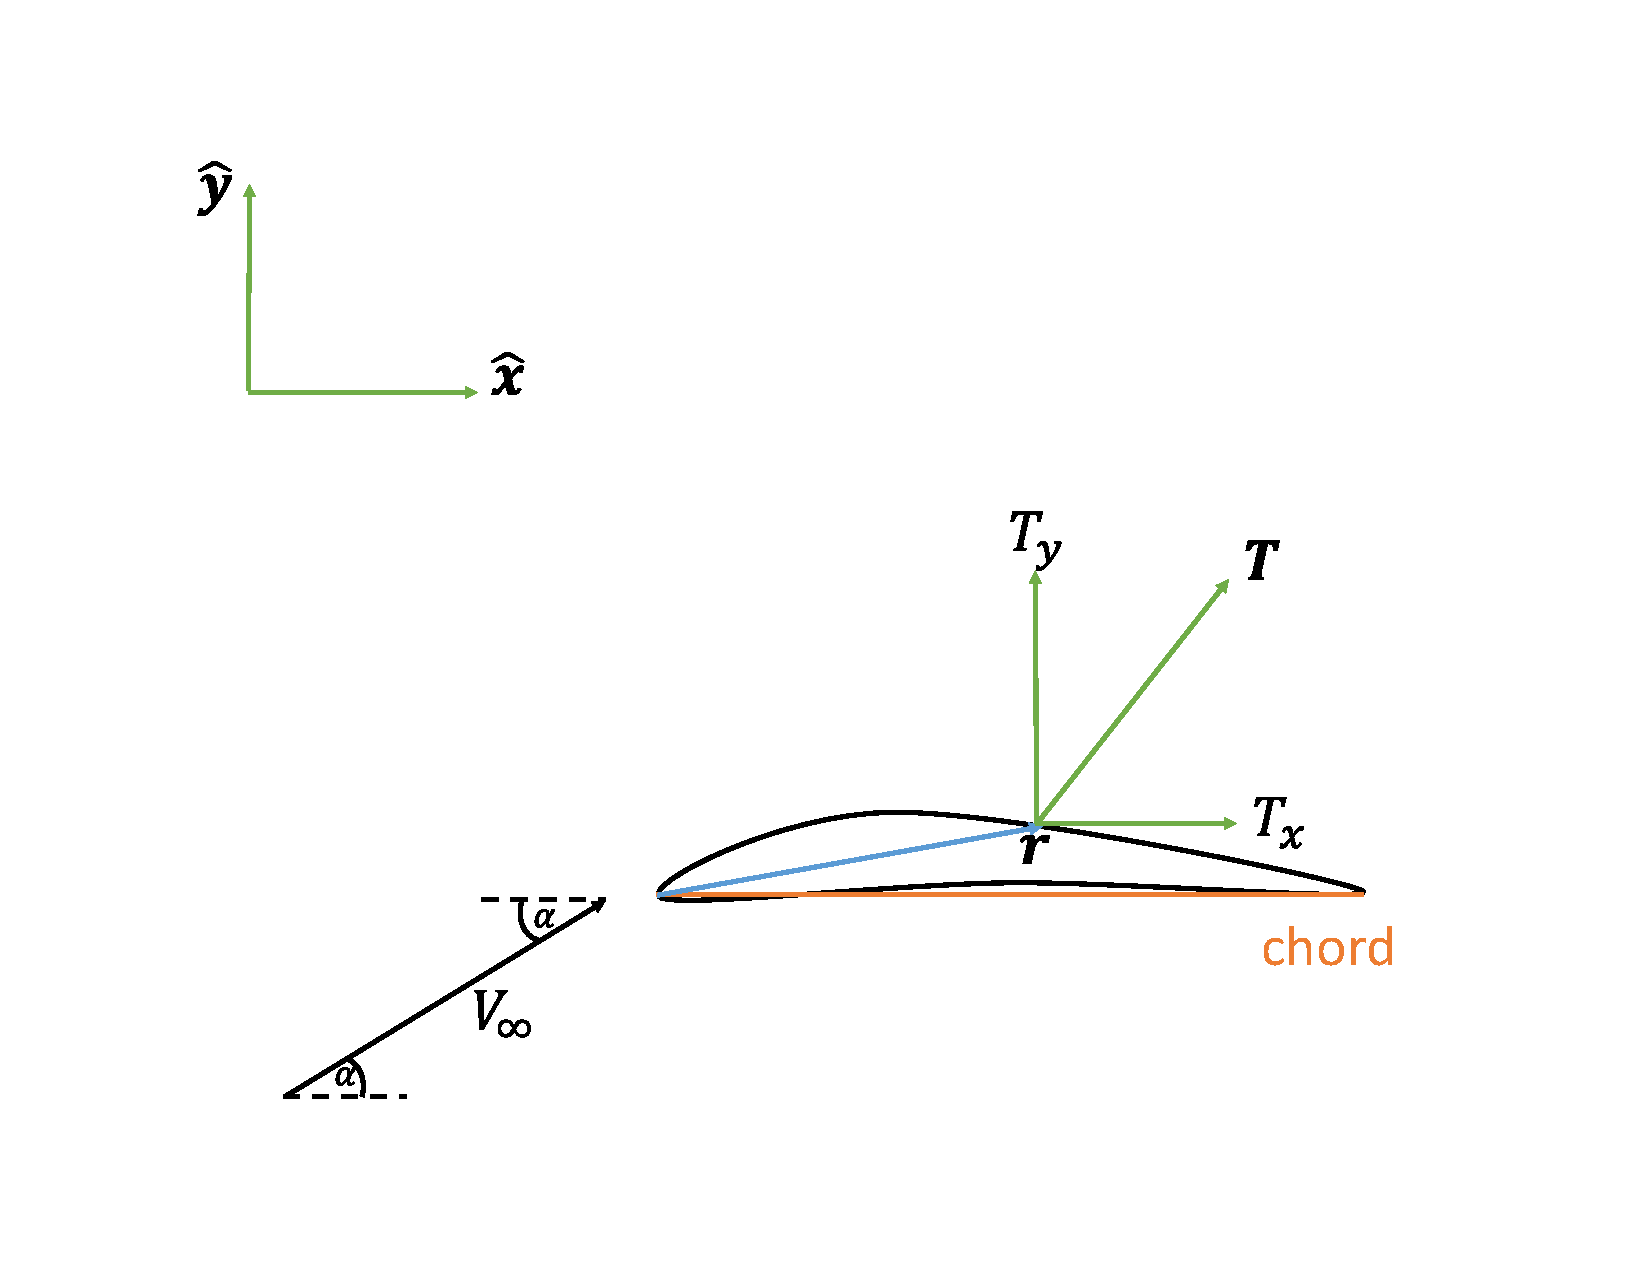
\includegraphics[width=0.8\textwidth]{../../images/airfoil.pdf}
   \caption{Coordinate system and representative forces on an airfoil.}
   \label{fig:airfoil}
\end{figure}

Consider the two dimensional case, as shown in \cref{fig:airfoil}. We label the normal force as
\begin{equation}
    F_N = \int_s T_y \, ds,
\end{equation}
and the tangential force as
\begin{equation}
    F_T = \int_s T_x \, ds.
\end{equation}
The moment about the leading edge, which points only along the $z$ direction only, can be written as
\begin{equation}
    M_{le} = \int_s (x \hat{\xvec} + y \hat{\yvec} ) \times (T_x \hat{\xvec} + T_y \hat{\yvec}) \, ds = \int_s x T_y - y T_x \, ds.
\end{equation}
Note that, for this convention, a positive moment decreases the angle of attach, and a negative moment increases the angle of attack---this is the opposite convention of Anderson. If we choose to compute the moment along an arbitrary point on the chord of the body, then \Cref{eq:moment_shift} becomes
\begin{equation}
    M_{ap} = M_{le} - x_{ap} F_N.
\end{equation}
The center of pressure is defined as the point along the chord for which the total moment becomes zero. Thus, it's location $x_{cp}$ is given by
\begin{equation}
    x_{cp} = \frac{M_{le}}{F_N}.
\end{equation}

The drag is defined as the force aligned with the free stream velocity, whereas the lift is the force normal to the free stream velocity. For 2D geometries, the direction of lift is well defined, whereas for 3D geometries, we pick the component of the force normal to the free stream velocity that points in the ``up'' direction. In terms for the normal and and tangential force, the lift and drag for a 2D geometry are given by
\begin{equation}
    \begin{bmatrix} L \\ D \end{bmatrix} = 
    \begin{bmatrix} \cos \alpha & \sin \alpha \\ -\sin \alpha & \cos \alpha \end{bmatrix} \begin{bmatrix} A \\ N \end{bmatrix}.
\end{equation}
Given the aerodynamics pressure
\begin{equation}
    q_\infty = \frac{1}{2} \rho_\infty V^2_\infty,
\end{equation}
a reference surface $S$, and a reference length $l$, the lift coefficient is given by
\begin{equation}
    C_L = \frac{L}{q_\infty S},
\end{equation}
the drag coefficient by
\begin{equation}
    C_D = \frac{L}{q_\infty S},
\end{equation}
and the moment coefficient by
\begin{equation}
    C_M = \frac{M}{q_\infty Sl}.
\end{equation}

%########################################################################
\chapter{Non-dimensionalization for compressible flows}
%########################################################################
Non-dimensionalization
\begin{align}
x_i = x^*_i L_0 &\qquad \qquad T = T^* T_0 \nonumber \\
t = t^* \frac{L_0}{u_0} &\qquad \qquad p = p^* \rho_0 u^2_0 \nonumber \\
\rho = \rho^* \rho_0 &\qquad \qquad \mu = \mu^* \mu_0 \nonumber \\
u_i = u^*_i u_0 &\qquad \qquad e = e^* u_0^2
\end{align}

Non-dimensional parameters
\begin{align}
    M_0 =& \frac{u_0}{c_0} \qquad \text{where } c_0 = \sqrt{\gamma R T_0} \\
    Re_0 =& \frac{\rho_0 u_0 l_0}{\mu_0}\\
    Pr_0 =& \frac{\mu_0 c_p}{\kappa_0}.
\end{align}

Parameters
\begin{align}
    M_t &= \frac{\sqrt{\langle u_i u_i \rangle}}{ \langle c \rangle} = \frac{\sqrt{\langle u_i u_i \rangle}}{ \langle \sqrt{\gamma R T} \rangle} = \frac{\sqrt{\langle u^*_i u^*_i \rangle}}{ \langle \sqrt{T^*} \rangle} \frac{u_0}{c_0} = \frac{\sqrt{\langle u^*_i u^*_i \rangle}}{ \langle \sqrt{T^*} \rangle} M_0 \\
    Re_\lambda &= \frac{\langle \rho \rangle u_{rms} \lambda }{\langle \mu \rangle} = \frac{\langle \rho^* \rangle u^*_{rms} \lambda^* }{\langle \mu^* \rangle} \frac{\rho_0 c_o L_0}{\mu_0} = \frac{\langle \rho^* \rangle u^*_{rms} \lambda^* }{\langle \mu^* \rangle} Re_0 \\
    Pr &= \frac{\mu c_p}{\kappa} = \frac{\mu^*}{\kappa^*} \frac{\mu_0 c_p}{\kappa_0} = \frac{\mu^*}{\kappa^*} Pr_0.
\end{align}

\newpage
Dimensional Navier-Stokes
\begin{equation}
\frac{\partial \rho}{\partial t} + \frac{\partial \rho u_i}{\partial x_i} = 0
\end{equation}
\begin{equation}
\frac{\partial \rho u_i}{\partial t} + \frac{\partial \rho u_i u_j}{\partial x_j} = -\frac{\partial p}{\partial x_i} + \frac{\partial \tau_{ij}}{\partial x_j}
\end{equation}
\begin{equation}
\frac{\partial \rho E}{\partial t} + \frac{\partial \rho E u_j}{\partial x_j} = -\frac{\partial u_j p}{\partial x_j} + \frac{\partial u_i \tau_{ij}}{\partial x_j} - \frac{\partial q_j}{\partial x_j}
\end{equation}
\begin{equation}
\tau_{ij} = 2 \mu \left (S_{ij} - \frac{1}{3} S_{kk} \delta_{ij} \right )
\end{equation}
\begin{equation}
p = \rho R T
\end{equation}
\begin{equation}
e = c_v T
\end{equation}
\begin{equation}
K = \frac{1}{2} u_i u_i
\end{equation}
\begin{equation}
q_j = -\kappa \frac{\partial T}{\partial x_j}
\end{equation}

Non-dimensional Navier-Stokes
\begin{equation}
\frac{\partial \rho^*}{\partial t^*} + \frac{\partial \rho^* u^*_i}{\partial x^*_i} = 0
\end{equation}
\begin{equation}
\frac{\partial \rho^* u^*_i}{\partial t^*} + \frac{\partial^* \rho^* u^*_i u^*_j}{\partial x^*_j} = -\frac{\partial p^*}{\partial x_i} + \frac{\partial \tau^*_{ij}}{\partial x^*_j}
\end{equation}
\begin{equation}
\frac{\partial \rho^* (e^* + K^*)}{\partial t^*} + \frac{\partial \rho^* (e^* + K^*) u^*_j}{\partial x^*_j} = -\frac{\partial u^*_j p^*}{\partial x^*_j} + \frac{\partial u^*_i \tau^*_{ij}}{\partial x^*_j} - \frac{\partial q^*_j}{\partial x^*_j}
\end{equation}
\begin{equation}
\tau^*_{ij} = 2 \frac{\mu^*}{Re_0} \left (S^*_{ij} - \frac{1}{3} S^*_{kk} \delta_{ij} \right )
\end{equation}
\begin{equation}
p^* = \frac{\rho^* T^*}{\gamma M_0^2}
\end{equation}
\begin{equation}
e^* = \frac{1}{\gamma (\gamma - 1) M_0^2} T^*
\end{equation}
\begin{equation}
K^* = e^* + \frac{1}{2} u_i^* u_i^*
\end{equation}
\begin{equation}
q_i^* = - \frac{\kappa^*}{(\gamma - 1) Pr_0 Re_0 M_0^2} \frac{ \partial T^*}{\partial x_i^*}
\end{equation}

\newpage
The variables needed are $\rho, u_i, T, R, \gamma, \mu, \kappa$.

Initial non-dimensional values
\begin{align}
\rho^* &= 1 \nonumber \\
u_i^* &= \text{spectrum with } \langle u^*_1 u^*_1 \rangle = \frac{1}{3} \nonumber \\
T^* &= \text{follows from }M_t \nonumber \\
\mu^* &= \left ( T^* \right)^{0.76}
\end{align}

Reference values
\begin{align}
L_0 &= 2 \pi \nonumber \\
\rho_0 &= 1 \nonumber \\
c_0 &= 1 \nonumber \\
T_0 &= \text{from }c_0 \nonumber \\
\mu_0 &= \text{from } Re_0
\end{align}

We then set $\gamma = 1.4$, $R = \frac{1}{\gamma}$ and compute $\kappa$ from $Pr$.

%########################################################################
\chapter{Helmholtz Decomposition}
%########################################################################
\begin{equation}
    \uvec = \uvec^{(s)} + \uvec^{(d)} + \uvec^{(h)}
\end{equation}
    
    We require
    \begin{align}
    \nabla \times \uvec^{(s)} = \wvec &\qquad \nabla \cdot \uvec^{(s)} = 0 \qquad \uvec^{(s)} = 0 \text{ on } \partial \Omega\\
    \nabla \times \uvec^{(d)} = 0 &\qquad \nabla \cdot \uvec^{(d)} = d \qquad \uvec^{(d)} = 0 \text{ on } \partial \Omega\\
    \nabla \times \uvec^{(h)} = 0 &\qquad \nabla \cdot \uvec^{(h)} = 0 \qquad \uvec^{(h)} = \uvec \text{ on } \partial \Omega
    \end{align}
    In other words, $\uvec^{(s)}$ accounts for the vorticity, $\uvec^{(d)}$ accounts for the dilatation, and $\uvec^{(h)}$ accounts for the boundary conditions.
    
    The above requirements allow us to write
    \begin{equation}
        \uvec^{(s)} = \nabla \times \psivec \qquad \uvec^{(d)} = \nabla \phi \qquad \uvec^{(h)} = \nabla \varphi 
    \end{equation}
    These potentials in turn can be solved using
    \begin{equation}
    \begin{cases}
    \nabla^2 \psivec = -\wvec & \text{in } \Omega \\
    \nabla \times \psivec = 0 & \text{on } \partial \Omega
    \end{cases}
    \end{equation}
    \begin{equation}
    \begin{cases}
    \nabla^2 \phi = d & \text{in } \Omega \\
    \nabla \phi = 0 & \text{on } \partial \Omega
    \end{cases}
    \end{equation}
    \begin{equation}
    \begin{cases}
    \nabla^2 \varphi = 0 & \text{in } \Omega \\
    \nabla \varphi = \uvec & \text{on } \partial \Omega
    \end{cases}
    \end{equation}
    assuming $\nabla \cdot \psivec = 0$.

    
\bibliographystyle{apalike}
\bibliography{library}

\end{document}